\documentclass[12pt]{article}
\markboth{ {\today}}{{\today}}
\pagestyle{myheadings}
\usepackage{amsmath}
\usepackage{epsfig}
 
\begin{document}
 
 
   
   
\newpage 
\setcounter{page}{ 
    26001 } 
   
   
   
   
\noindent\begin{tabular}{|l|}
\hline
YOUR NAME (FIRST, ... LAST)  \\
\hline
 \\ 
 \\ 
\hline
\end{tabular}
\hspace{0.05in} \begin{tabular}{|l|}
\hline
 YOUR   ID   INFORMATION  \\
\hline
 \\ 
 \\ 
\hline
\end{tabular}
   
   
\vspace{0.2in}\noindent\begin{tabular}{|l|}
\hline
YOUR TOTAL MARKS  \\
\hline
 \\ 
 \\ 
\hline
\end{tabular}
\hspace{0.05in} \begin{tabular}{|l|}
\hline
TOTAL FULL MARKS  \\
\hline
 \\ 
100.00 \\
\hline
\end{tabular}
   
   
 \vspace{0.2in}
 
 
{\Huge  THIS IS AN EXAMPLE OF}
 
{\Huge  PERSONALIZED TESTS. }
 
If needed, please use the following constants.
 
 
 
\noindent\begin{tabular}{|l|l|l|}
\hline
Constant & Symbol & Value \\
\hline
Acceleration due to earth's gravity &
$g$ &
 $ 9.80 $
m/s$^2$ \\
\hline
Avogadro's number &
$N_A$ &
 $ 6.0221367 \times 10^{23} $
mol$^{-1}$ \\
\hline
Boltzmann's constant &
$k$ &
 $ 1.380658 \times 10^{-23} $
J/K \\
\hline
Coulomb's constant &
$k$ &
 $ 8.99 \times 10^{9} $
N$\cdot $m$^2$/C$^2$ \\
\hline
Electron charge magnitiude &
$e$ &
 $ 1.60217733 \times 10^{-19} $
C \\
\hline
Permeability of free space &
$\mu _0$ &
 $ 1.25663706 \times 10^{-6} $
T$\cdot $m/A \\
\hline
Permittivity of free space &
$\epsilon _0$ &
 $ 8.854187817 \times 10^{-12} $
C$^2$/(N$\cdot $m$^2$) \\
\hline
Pi &
$\pi$ &
 $ 3.14159265 $
$ $ \\
\hline
Planck's constant &
$h$ &
 $ 6.6260755 \times 10^{-34} $
J$\cdot $s \\
\hline
Mass of electron &
$m_e$ &
 $ 9.1093897 \times 10^{-31} $
kg \\
\hline
\end{tabular}
 
 
\noindent\begin{tabular}{|l|l|l|}
\hline
Constant & Symbol & Value \\
\hline
Mass of neutron &
$m_n$ &
 $ 1.6749286 \times 10^{-27} $
kg \\
\hline
Mass of proton &
$m_p$ &
 $ 1.6726231 \times 10^{-27} $
kg \\
\hline
Speed of light in vacuum &
$c$ &
 $ 299792458. $
m/s \\
\hline
Universal gravitational constant &
$G$ &
 $ 6.67259 \times 10^{-11} $
N$\cdot $m$^2$/kg$^2$ \\
\hline
Universal gas constant &
$R$ &
 $ 8.314510 $
J/(mol$\cdot $K) \\
\hline
\end{tabular}
 
 
{\textbf{\large{Please be advised}}} that in this paper there are questions from
26.1 through
26.9.
And any one of them may contain more than one sub-question, thus the total number
of sub-questions here is around 14, of which
13 should be answered.
 
\vspace{0.3in}
 
 
   
   
  
\vspace{0.2in}
  
\noindent\begin{tabular}{|l|}
\hline
 YOUR MARKS  \\
\hline
 \\ 
 \\ 
\hline
\end{tabular}
\hspace{0.05in} \begin{tabular}{|l|}
\hline
 Full Marks  \\
\hline
 \\ 
62.50 \\
\hline
\end{tabular}
{\textbf{\Large{QUESTION
26.1 
}}}
  
  
 
{\textbf{\Large{Please answer ONLY
5 of the following
6 questions (Questions
26.1.1 through
26.1.6). }}}
 
Here are still some constants for use in the following questions:
 
 
\noindent\begin{tabular}{|l|l|l|}
\hline
Constant & Symbol & Value \\
\hline
 
Boltzmann's constant &
$k$ &
 $ 1.381 \times 10^{-23} $
J/K \\
\hline
 
Avogadro's number &
$N_A$ &
 $ 6.022 \times 10^{23} $
mol$^{-1}$ \\
\hline
 
Mass of electron &
$m_e$ &
 $ 9.1093897 \times 10^{-31} $
kg \\
\hline
 
\end{tabular}
 
  
\vspace{0.2in}
  
         \begin{tabular}{|l|}
\hline
 Your marks  \\
\hline
 \\ 
 \\ 
\hline
\end{tabular}
\hspace{0.05in} \begin{tabular}{|l|}
\hline
 Full marks  \\
\hline
 \\ 
12.50 \\
\hline
\end{tabular}
{\textbf{\Large{Question
26.1.1 
}}}
  
  
See the following picture.
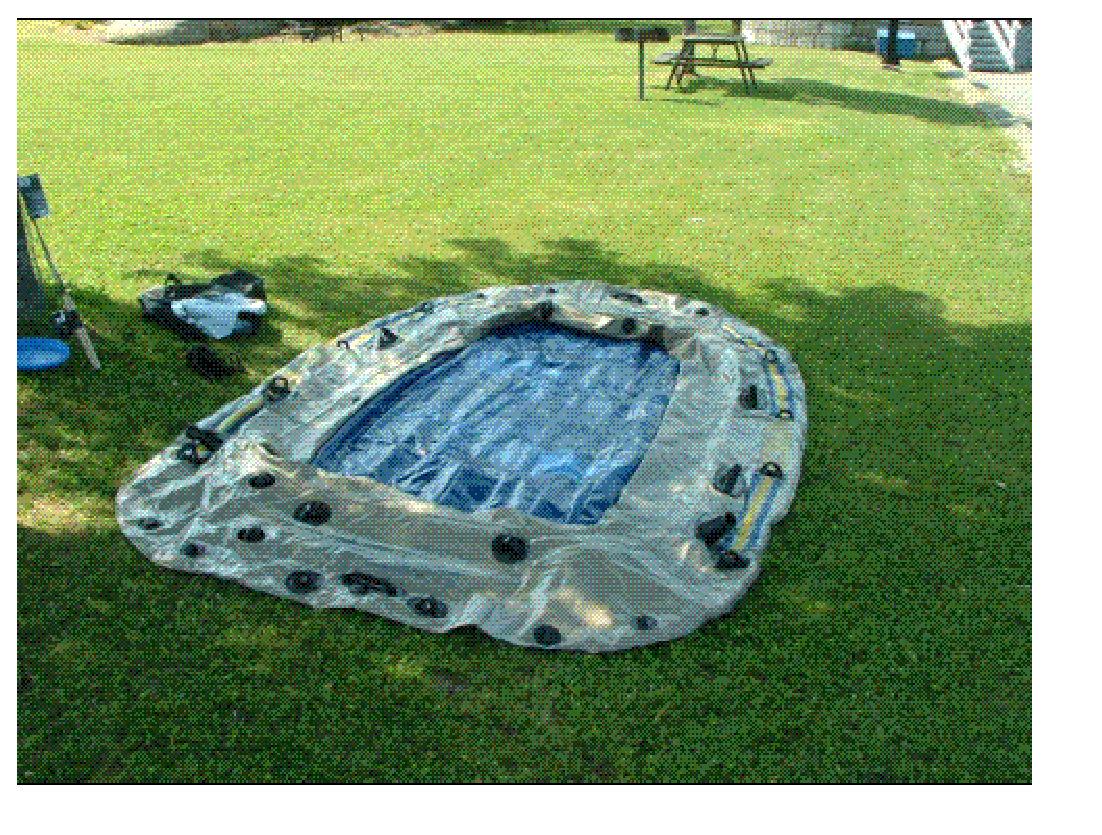
\epsfig{file=fig1.eps,width=3.5in}
Which one of the following is missing in it?
  
  
\noindent\hspace{3.0in} \begin{tabular}{|l|}
\hline
Your choice \\
\hline
 \\ 
 \\ 
\hline
\end{tabular}
  
  
 
 
\noindent{\textbf{\large{
A.}}}
An air-boat
 
 
\noindent{\textbf{\large{
B.}}}
Lawn
 
 
\noindent{\textbf{\large{
C.}}}
A table
 
 
\noindent{\textbf{\large{
D.}}}
A truck
 
 
\noindent{\textbf{\large{
E.}}}
An airplane
 
 
\noindent{\textbf{\large{
F.}}}
  Not any of aboves.
 
 
 
\vspace{0.3in}
  
\vspace{0.2in}
  
         \begin{tabular}{|l|}
\hline
 Your marks  \\
\hline
 \\ 
 \\ 
\hline
\end{tabular}
\hspace{0.05in} \begin{tabular}{|l|}
\hline
 Full marks  \\
\hline
 \\ 
12.50 \\
\hline
\end{tabular}
{\textbf{\Large{Question
26.1.2 
}}}
  
  
In a hotel, the possiblity of  % 
non-smoking customer is
$a =  % 
0.270$, and the possiblity of  % 
equal or above 30 years old customer is $ b =  % 
0.5200$.
Please calculate the possiblity of  % 
smoking and  % 
under 30 years old customer.
 

 

 
\vspace{0.3in}
  
\vspace{0.2in}
  
         \begin{tabular}{|l|}
\hline
 Your marks  \\
\hline
 \\ 
 \\ 
\hline
\end{tabular}
\hspace{0.05in} \begin{tabular}{|l|}
\hline
 Full marks  \\
\hline
 \\ 
12.50 \\
\hline
\end{tabular}
{\textbf{\Large{Question
26.1.3 
}}}
  
  
What is the operation between $a= % 
3$ and $b= % 
2$:
$a$  % 
$+$ $b=?$ Please also calculate it.

 
\vspace{0.3in}
  
\vspace{0.2in}
  
         \begin{tabular}{|l|}
\hline
 Your marks  \\
\hline
 \\ 
 \\ 
\hline
\end{tabular}
\hspace{0.05in} \begin{tabular}{|l|}
\hline
 Full marks  \\
\hline
 \\ 
12.50 \\
\hline
\end{tabular}
{\textbf{\Large{Question
26.1.4 
}}}
  
  
Let us use Newton's Law of Universal Gravitation to calculate the force
of the Sun acting on the eight planets. Let us suppose the mass of the
Sun is $ % 
7.00 \times 10^{24} kg$. With the mass and the
distance to the Sun of each planet in the following table, please fill
the blanks for the forces.
 
\vspace{0.2in}
 
 
\begin{tabular}{|l|l|l|l|}
\hline
The Planet & Mass ($kg$) & Distanace from Sun ($m$) & The Force ($N$)\\
\hline
Mercury  &
           $ % 
2.00000000 \times 10^{24} $   &
             $ % 
5.000000000 \times 10^{24} $    &
\\  \hline
Venus    &
           $ % 
8.00 \times 10^{24} $    &
             $ % 
6.00 \times 10^{24} $    &
\\  \hline
Earth    &
           $ % 
9.00 \times 10^{24} $    &
             $ % 
3.00 \times 10^{24} $    &
\\   \hline
Mars     &
           $ % 
9.00 \times 10^{24} $    &
             $ % 
4.00 \times 10^{24} $    &
\\   \hline
Jupiter  &
           $ % 
2.00 \times 10^{24} $    &
             $ % 
3.00 \times 10^{24} $    &
\\  \hline
Saturn   &
           $ % 
9.00 \times 10^{24}$    &
             $ % 
6.00 \times 10^{24}$    &
\\  \hline
Uranus   &
           $ % 
8.00 \times 10^{24} $    &
             $ % 
7.00 \times 10^{24} $    &
\\  \hline
Neptune  &
           $ % 
5.00 \times 10^{24} $    &
             $ % 
4.00 \times 10^{24} $    &
\\  \hline
 
\end{tabular}
 
 

 
 

 
\vspace{0.3in}
  
\vspace{0.2in}
  
         \begin{tabular}{|l|}
\hline
 Your marks  \\
\hline
 \\ 
 \\ 
\hline
\end{tabular}
\hspace{0.05in} \begin{tabular}{|l|}
\hline
 Full marks  \\
\hline
 \\ 
12.50 \\
\hline
\end{tabular}
{\textbf{\Large{Question
26.1.5 
}}}
  
  
 
An object is subjected to an external net force $\mathbf{f}=(
80.0 ,
3.0,
-3000.0  )N$. Its mass is known as
$m= % 
52.0  kg$. Please choose the correct accelaration
from the following choices.
 
  
  
\noindent\hspace{3.0in} \begin{tabular}{|l|}
\hline
Your choice \\
\hline
 \\ 
 \\ 
\hline
\end{tabular}
  
  
 
 
\noindent{\textbf{\large{
A.}}}
The accelaration is
$(
6.6592ms^{-2},
5.7692 \times 10^{-2}ms^{-2},
-2.5735 \times 10^{6}km/h^2
).
$
 
 
\noindent{\textbf{\large{
B.}}}
The accelaration is
$(
6.6592ms^{-2},
-0.12162ms^{-2},
-2.5735 \times 10^{6}km/h^2
).
$
 
 
\noindent{\textbf{\large{
C.}}}
The accelaration is
$(
6.6592ms^{-2},
5.7692 \times 10^{-2}ms^{-2},
-747692.km/h^2
).
$
 
 
\noindent{\textbf{\large{
D.}}}
The accelaration is
$(
1.5385ms^{-2},
5.7692 \times 10^{-2}ms^{-2},
-747692.km/h^2
).
$
 
 
\noindent{\textbf{\large{
E.}}}
none of these.
 
 
 
 

 
\vspace{0.3in}
  
\vspace{0.2in}
  
         \begin{tabular}{|l|}
\hline
 Your marks  \\
\hline
 \\ 
 \\ 
\hline
\end{tabular}
\hspace{0.05in} \begin{tabular}{|l|}
\hline
 Full marks  \\
\hline
 \\ 
12.50 \\
\hline
\end{tabular}
{\textbf{\Large{Question
26.1.6 
}}}
  
  
 
An object is subjected to an external net force $\mathbf{f}=(
90.0 ,
2.0,
-7000.0  )N$. Its mass is known as
$m= % 
56.0  kg$. Please choose the correct accelaration
from the following choices.
 
  
  
\noindent\hspace{3.0in} \begin{tabular}{|l|}
\hline
Your choice \\
\hline
 \\ 
 \\ 
\hline
\end{tabular}
  
  
 
 
\noindent{\textbf{\large{
A.}}}
The accelaration (vector) is
$(
-103670.,
462.86 ,
4.9517 \times 10^{6}
)km/h^2.
$
 
 
\noindent{\textbf{\large{
B.}}}
The accelaration (vector) is
$(
55447.,
462.86 ,
6.8897 \times 10^{6}
)km/h^2.
$
 
 
\noindent{\textbf{\large{
C.}}}
The accelaration (vector) is
$(
55447.,
462.86 ,
-1.6200 \times 10^{6}
)km/h^2.
$
 
 
\noindent{\textbf{\large{
D.}}}
The accelaration (vector) is
$(
20829.,
462.86 ,
-1.6200 \times 10^{6}
)km/h^2.
$
 
 
\noindent{\textbf{\large{
E.}}}
The accelaration (vector) is
$(
20829.,
462.86 ,
6.8897 \times 10^{6}
)km/h^2.
$
 
 
\noindent{\textbf{\large{
F.}}}
The accelaration (vector) is
$(
-103670.,
462.86 ,
6.8897 \times 10^{6}
)km/h^2.
$
 
 
\noindent{\textbf{\large{
G.}}}
The accelaration (vector) is
$(
20829.,
462.86 ,
4.1819 \times 10^{6}
)km/h^2.
$
 
 
\noindent{\textbf{\large{
H.}}}
The accelaration (vector) is
$(
71153.,
462.86 ,
4.1819 \times 10^{6}
)km/h^2.
$
 
 
\noindent{\textbf{\large{
I.}}}
The accelaration (vector) is
$(
55447.,
462.86 ,
4.9517 \times 10^{6}
)km/h^2.
$
 
 
\noindent{\textbf{\large{
J.}}}
The accelaration (vector) is
$(
-103670.,
462.86 ,
4.1819 \times 10^{6}
)km/h^2.
$
 
 
\noindent{\textbf{\large{
K.}}}
The accelaration (vector) is
$(
71153.,
462.86 ,
4.9517 \times 10^{6}
)km/h^2.
$
 
 
\noindent{\textbf{\large{
L.}}}
The accelaration (vector) is
$(
-103670.,
462.86 ,
-1.6200 \times 10^{6}
)km/h^2.
$
 
 
 
 

 
 
\vspace{0.3in}
   
   
\vspace{0.3in}
{\textbf{\LARGE{You have done all the above? A very good beginning, please go ahead.}}}
More constants the
Mass of electron
$m_e$$ =
9.109390 \times 10^{-31} $
kg
,
Universal gas constant
$R$$ =
8.315 $
J/(mol$\cdot $K)
,
$e$$ =
1.60217733 \times 10^{-19} $
C
, and
$m_p$$ =
1.6726231 \times 10^{-27} $
kg
%
may be very helpful.
\vspace{0.3in}
   
   
  
\vspace{0.2in}
  
\noindent\begin{tabular}{|l|}
\hline
 YOUR MARKS  \\
\hline
 \\ 
 \\ 
\hline
\end{tabular}
\hspace{0.05in} \begin{tabular}{|l|}
\hline
 Full Marks  \\
\hline
 \\ 
1.56 \\
\hline
\end{tabular}
{\textbf{\Large{QUESTION
26.2 
}}}
  
  
If any one of the following statements is correct, please fill the box ahead of it with $T$ .
If wrong, fill with $F$.
 
\noindent\begin{tabular}{|l|l|}\hline Your&\hspace{.2in} \\ answer&\hspace{.2in} \\ \hline \end{tabular}
1. $ % 
96$ is an  % 
even number.
 
\noindent\begin{tabular}{|l|l|}\hline Your&\hspace{.2in} \\ answer&\hspace{.2in} \\ \hline \end{tabular}
2.  % 
Toronto is in  % 
Ontario province.
 
\noindent\begin{tabular}{|l|l|}\hline Your&\hspace{.2in} \\ answer&\hspace{.2in} \\ \hline \end{tabular}
3.  % 
$\left| \mathbf{F}\right| =Gm_1m_2r^{-2}$ is a mathmatical form of
the Newton's Second Law.
 

 
\vspace{0.3in}
  
\vspace{0.2in}
  
\noindent\begin{tabular}{|l|}
\hline
 YOUR MARKS  \\
\hline
 \\ 
 \\ 
\hline
\end{tabular}
\hspace{0.05in} \begin{tabular}{|l|}
\hline
 Full Marks  \\
\hline
 \\ 
1.56 \\
\hline
\end{tabular}
{\textbf{\Large{QUESTION
26.3 
}}}
  
  
Please choose the correct one from the following statements:
  
  
\noindent\hspace{3.0in} \begin{tabular}{|l|}
\hline
Your choice \\
\hline
 \\ 
 \\ 
\hline
\end{tabular}
  
  
 
 
\noindent{\textbf{\large{
A.}}}
Canada has  %
34 provinces and  %
39 territories.
 
 
\noindent{\textbf{\large{
B.}}}
Canada has  %
37 provinces and  %
37 territories.
 
 
\noindent{\textbf{\large{
C.}}}
Canada has  %
36 provinces and  %
35 territories.
 
 
\noindent{\textbf{\large{
D.}}}
Canada has  %
33 provinces and  %
38 territories.
 
 
\noindent{\textbf{\large{
E.}}}
Canada has  %
35 provinces and  %
34 territories.
 
 
\noindent{\textbf{\large{
F.}}}
 None of above.
 
 
  
\vspace{0.2in}
  
\noindent\begin{tabular}{|l|}
\hline
 YOUR MARKS  \\
\hline
 \\ 
 \\ 
\hline
\end{tabular}
\hspace{0.05in} \begin{tabular}{|l|}
\hline
 Full Marks  \\
\hline
 \\ 
1.56 \\
\hline
\end{tabular}
{\textbf{\Large{QUESTION
26.4 
}}}
  
  
 
An object is subjected to an external net force $\mathbf{f}=(
30.000 ,
3.0000,
-9000.0  )N$. Its mass is known as
$m= % 
52.0000  kg$. Please choose the correct accelaration
from the following choices.
 
  
  
\noindent\hspace{3.0in} \begin{tabular}{|l|}
\hline
Your choice \\
\hline
 \\ 
 \\ 
\hline
\end{tabular}
  
  
 
 
\noindent{\textbf{\large{
A.}}}
The accelaration is
$(
-1.9975ms^{-2},
747.69km/h^2,
554.32ms^{-2}
).
$
 
 
\noindent{\textbf{\large{
B.}}}
The accelaration is
$(
-1.9975ms^{-2},
3540.9km/h^2,
-173.08ms^{-2}
).
$
 
 
\noindent{\textbf{\large{
C.}}}
The accelaration is
$(
-1.9975ms^{-2},
3540.9km/h^2,
554.32ms^{-2}
).
$
 
 
\noindent{\textbf{\large{
D.}}}
The accelaration is
$(
0.57692ms^{-2},
3540.9km/h^2,
-173.08ms^{-2}
).
$
 
 
\noindent{\textbf{\large{
E.}}}
The accelaration is
$(
-1.9975ms^{-2},
747.69km/h^2,
-173.08ms^{-2}
).
$
 
 
\noindent{\textbf{\large{
F.}}}
The accelaration is
$(
0.57692ms^{-2},
3540.9km/h^2,
554.32ms^{-2}
).
$
 
 
\noindent{\textbf{\large{
G.}}}
 None of these.
 
 
 
 

 
\vspace{0.3in}
  
\vspace{0.2in}
  
\noindent\begin{tabular}{|l|}
\hline
 YOUR MARKS  \\
\hline
 \\ 
 \\ 
\hline
\end{tabular}
\hspace{0.05in} \begin{tabular}{|l|}
\hline
 Full Marks  \\
\hline
 \\ 
3.12 \\
\hline
\end{tabular}
{\textbf{\Large{QUESTION
26.5 
}}}
  
  
 
 
An object is subjected to an external net force $\mathbf{f}=
(20.0 , 7.0 , -9000.0) N$.
Its mass is known as $m= % 
54.0000 kg$. Please choose the
correct accelaration from the following choices.
 
  
  
\noindent\hspace{3.0in} \begin{tabular}{|l|}
\hline
Your choice \\
\hline
 \\ 
 \\ 
\hline
\end{tabular}
  
  
 
 
\noindent{\textbf{\large{
A.}}}
The accelaration is $  %
(
0.370,
0.26,
-166.67)
ms^{-2} $.
 
 
\noindent{\textbf{\large{
B.}}}
The accelaration is $  %
(
4.13,
0.26,
397.85)
ms^{-2} $.
 
 
\noindent{\textbf{\large{
C.}}}
The accelaration is $  %
(
4.13,
0.13,
-166.67)
ms^{-2} $.
 
 
\noindent{\textbf{\large{
D.}}}
The accelaration is $  %
(
0.370,
0.26,
397.85)
ms^{-2} $.
 
 
\noindent{\textbf{\large{
E.}}}
The accelaration is $  %
(
0.370,
0.13,
397.85)
ms^{-2} $.
 
 
\noindent{\textbf{\large{
F.}}}
The accelaration is $  %
(
0.370,
0.13,
-166.67)
ms^{-2} $.
 
 
\noindent{\textbf{\large{
G.}}}
The accelaration is $  %
(
4.13,
0.13,
397.85)
ms^{-2} $.
 
 
\noindent{\textbf{\large{
H.}}}
The accelaration is $  %
(
4.13,
0.26,
-166.67)
ms^{-2} $.
 
 
 

 

 
\vspace{0.3in}
  
\vspace{0.2in}
  
\noindent\begin{tabular}{|l|}
\hline
 YOUR MARKS  \\
\hline
 \\ 
 \\ 
\hline
\end{tabular}
\hspace{0.05in} \begin{tabular}{|l|}
\hline
 Full Marks  \\
\hline
 \\ 
3.12 \\
\hline
\end{tabular}
{\textbf{\Large{QUESTION
26.6 
}}}
  
  
Considering case-insensitivity, please match the following same strings.
  
  
\begin{tabular}{|l|l|l|}
 \hline
 Column Left & Column Right  & Your choinces \\ 
 \hline
{\textbf{\large{
A.}}}
A
  & 
a
 & 
 \\ 
 \hline
{\textbf{\large{
B.}}}
C
  & 
eR
 & 
 \\ 
 \hline
{\textbf{\large{
C.}}}
er
  & 
ER
 & 
 \\ 
 \hline
{\textbf{\large{
D.}}}
Er
  & 
c
 & 
 \\ 
 \hline
{\textbf{\large{
E.}}}
asdf(:)
  & 
ASDF(:)
 & 
 \\ 
 \hline
 \end{tabular}
  
  
 
   
   
\vspace{0.3in}
{\textbf{\LARGE{You have done all the above? Excellent! Not much left, please continue.}}}
\vspace{0.3in}
   
   
  
\vspace{0.2in}
  
\noindent\begin{tabular}{|l|}
\hline
 YOUR MARKS  \\
\hline
 \\ 
 \\ 
\hline
\end{tabular}
\hspace{0.05in} \begin{tabular}{|l|}
\hline
 Full Marks  \\
\hline
 \\ 
12.50 \\
\hline
\end{tabular}
{\textbf{\Large{QUESTION
26.7 
}}}
  
  
 
An object is subjected to an external net force $\mathbf{f}=
(90.0 , 9.0 , -5000.0) N$.
Its mass is known as $m= % 
54.0 kg$.
Please choose the correct accelaration from the following choices.
  
  
\noindent\hspace{3.0in} \begin{tabular}{|l|}
\hline
Your choice \\
\hline
 \\ 
 \\ 
\hline
\end{tabular}
  
  
 
 
\noindent{\textbf{\large{
A.}}}
  The accelaration is $  %
(
1.67,
0.17,
-92.593)
ms^{-2} $.
 
 
\noindent{\textbf{\large{
B.}}}
  The accelaration is $  %
(
4.19,
0.17,
-92.593)
ms^{-2} $.
 
 
\noindent{\textbf{\large{
C.}}}
  The accelaration is $  %
(
4.19,
-0.58,
242.38)
ms^{-2} $.
 
 
\noindent{\textbf{\large{
D.}}}
  The accelaration is $  %
(
1.67,
0.17,
242.38)
ms^{-2} $.
 
 
 

 
 
\vspace{0.3in}
  
\vspace{0.2in}
  
\noindent\begin{tabular}{|l|}
\hline
 YOUR MARKS  \\
\hline
 \\ 
 \\ 
\hline
\end{tabular}
\hspace{0.05in} \begin{tabular}{|l|}
\hline
 Full Marks  \\
\hline
 \\ 
12.50 \\
\hline
\end{tabular}
{\textbf{\Large{QUESTION
26.8 
}}}
  
  
 
$ \left( \begin{array}{ccccccccc}
           4  & 
           7  & 
           5  & 
           4  \\ 
           4  & 
           4  & 
           4  & 
           4  \\ 
           5  & 
           6  & 
           5  & 
           5
\end{array}\right) \times
\left( \begin{array}{c}
           2  \\ 
           2  \\ 
           2  \\ 
           2
\end{array}\right) $ =?
 
 
$  % 
 \left( \begin{array}
 {
 c
 c
 }
 \Theta & 
                    \zeta \\ 
 \Phi & 
 \eta \\ 
 \Theta & 
 \Upsilon \\ 
 \Delta & 
                    \Xi
 \end{array} \right)
 \left( \begin{array}
 {
 c
 }
 \beta \\ 
 \gamma
 \end{array} \right)
$ =?
 

 

 
\vspace{0.3in}
  
\vspace{0.2in}
  
\noindent\begin{tabular}{|l|}
\hline
 YOUR MARKS  \\
\hline
 \\ 
 \\ 
\hline
\end{tabular}
\hspace{0.05in} \begin{tabular}{|l|}
\hline
 Full Marks  \\
\hline
 \\ 
1.56 \\
\hline
\end{tabular}
{\textbf{\Large{QUESTION
26.9 
}}}
  
  
 
 
% First root
% Second root

 
Please solve the following equation:
\begin{eqnarray*}
-11 \times x^2  % 
-154
                 \times x    % 
-539 =0
\end{eqnarray*}
 

 

 
\vspace{0.3in}
   
   
 \vspace{0.2in}
Here are still some constants for use:
 
 
\noindent\begin{tabular}{|l|l|l|}
\hline
Constant & Symbol & Value \\
\hline
 
Mass of proton &
$m_p$ &
 $ 1.6726231 \times 10^{-27} $
kg \\
\hline
 
Boltzmann's constant &
$k$ &
 $ 1.381 \times 10^{-23} $
J/K \\
\hline
 
\end{tabular}
 
Thank you very much for answering these questions!
 
{\textbf{\large{Please be advised}}} that in this paper there are questions from
26.1 through
26.9.
And any one of them may contain more than one sub-question, thus the total number
of sub-questions here is around 14, of which
13 should be answered.
 
   
   
   
   
\vspace{1.0in} 
{\textbf{\large{ *** END OF PAPER, THANKS *** }}} 
   
   
\hspace{1.0in} By: 
         239 (          26 ,           34 )
   
   
   
   
\newpage 
\setcounter{page}{ 
    27001 } 
   
   
   
   
\noindent\begin{tabular}{|l|}
\hline
YOUR NAME (FIRST, ... LAST)  \\
\hline
 \\ 
 \\ 
\hline
\end{tabular}
\hspace{0.05in} \begin{tabular}{|l|}
\hline
 YOUR   ID   INFORMATION  \\
\hline
 \\ 
 \\ 
\hline
\end{tabular}
   
   
\vspace{0.2in}\noindent\begin{tabular}{|l|}
\hline
YOUR TOTAL MARKS  \\
\hline
 \\ 
 \\ 
\hline
\end{tabular}
\hspace{0.05in} \begin{tabular}{|l|}
\hline
TOTAL FULL MARKS  \\
\hline
 \\ 
100.00 \\
\hline
\end{tabular}
   
   
 \vspace{0.2in}
 
 
{\Huge  THIS IS AN EXAMPLE OF}
 
{\Huge  PERSONALIZED TESTS. }
 
If needed, please use the following constants.
 
 
 
\noindent\begin{tabular}{|l|l|l|}
\hline
Constant & Symbol & Value \\
\hline
Acceleration due to earth's gravity &
$g$ &
 $ 9.80 $
m/s$^2$ \\
\hline
Avogadro's number &
$N_A$ &
 $ 6.0221367 \times 10^{23} $
mol$^{-1}$ \\
\hline
Boltzmann's constant &
$k$ &
 $ 1.380658 \times 10^{-23} $
J/K \\
\hline
Coulomb's constant &
$k$ &
 $ 8.99 \times 10^{9} $
N$\cdot $m$^2$/C$^2$ \\
\hline
Electron charge magnitiude &
$e$ &
 $ 1.60217733 \times 10^{-19} $
C \\
\hline
Permeability of free space &
$\mu _0$ &
 $ 1.25663706 \times 10^{-6} $
T$\cdot $m/A \\
\hline
Permittivity of free space &
$\epsilon _0$ &
 $ 8.854187817 \times 10^{-12} $
C$^2$/(N$\cdot $m$^2$) \\
\hline
Pi &
$\pi$ &
 $ 3.14159265 $
$ $ \\
\hline
Planck's constant &
$h$ &
 $ 6.6260755 \times 10^{-34} $
J$\cdot $s \\
\hline
Mass of electron &
$m_e$ &
 $ 9.1093897 \times 10^{-31} $
kg \\
\hline
\end{tabular}
 
 
\noindent\begin{tabular}{|l|l|l|}
\hline
Constant & Symbol & Value \\
\hline
Mass of neutron &
$m_n$ &
 $ 1.6749286 \times 10^{-27} $
kg \\
\hline
Mass of proton &
$m_p$ &
 $ 1.6726231 \times 10^{-27} $
kg \\
\hline
Speed of light in vacuum &
$c$ &
 $ 299792458. $
m/s \\
\hline
Universal gravitational constant &
$G$ &
 $ 6.67259 \times 10^{-11} $
N$\cdot $m$^2$/kg$^2$ \\
\hline
Universal gas constant &
$R$ &
 $ 8.314510 $
J/(mol$\cdot $K) \\
\hline
\end{tabular}
 
 
{\textbf{\large{Please be advised}}} that in this paper there are questions from
27.1 through
27.9.
And any one of them may contain more than one sub-question, thus the total number
of sub-questions here is around 14, of which
13 should be answered.
 
\vspace{0.3in}
 
 
   
   
  
\vspace{0.2in}
  
\noindent\begin{tabular}{|l|}
\hline
 YOUR MARKS  \\
\hline
 \\ 
 \\ 
\hline
\end{tabular}
\hspace{0.05in} \begin{tabular}{|l|}
\hline
 Full Marks  \\
\hline
 \\ 
62.50 \\
\hline
\end{tabular}
{\textbf{\Large{QUESTION
27.1 
}}}
  
  
 
{\textbf{\Large{Please answer ONLY
5 of the following
6 questions (Questions
27.1.1 through
27.1.6). }}}
 
Here are still some constants for use in the following questions:
 
 
\noindent\begin{tabular}{|l|l|l|}
\hline
Constant & Symbol & Value \\
\hline
 
Boltzmann's constant &
$k$ &
 $ 1.381 \times 10^{-23} $
J/K \\
\hline
 
Avogadro's number &
$N_A$ &
 $ 6.022 \times 10^{23} $
mol$^{-1}$ \\
\hline
 
Mass of electron &
$m_e$ &
 $ 9.1093897 \times 10^{-31} $
kg \\
\hline
 
\end{tabular}
 
  
\vspace{0.2in}
  
         \begin{tabular}{|l|}
\hline
 Your marks  \\
\hline
 \\ 
 \\ 
\hline
\end{tabular}
\hspace{0.05in} \begin{tabular}{|l|}
\hline
 Full marks  \\
\hline
 \\ 
12.50 \\
\hline
\end{tabular}
{\textbf{\Large{Question
27.1.1 
}}}
  
  
 
An object is subjected to an external net force $\mathbf{f}=(
40.0,  % 
7.0,
-7000.0  )N$. Its mass is known as
$m= % 
52.0 kg$. Please calculate its accelaration.
 
 

 

 
\vspace{0.3in}
  
\vspace{0.2in}
  
         \begin{tabular}{|l|}
\hline
 Your marks  \\
\hline
 \\ 
 \\ 
\hline
\end{tabular}
\hspace{0.05in} \begin{tabular}{|l|}
\hline
 Full marks  \\
\hline
 \\ 
12.50 \\
\hline
\end{tabular}
{\textbf{\Large{Question
27.1.2 
}}}
  
  
See the following picture.
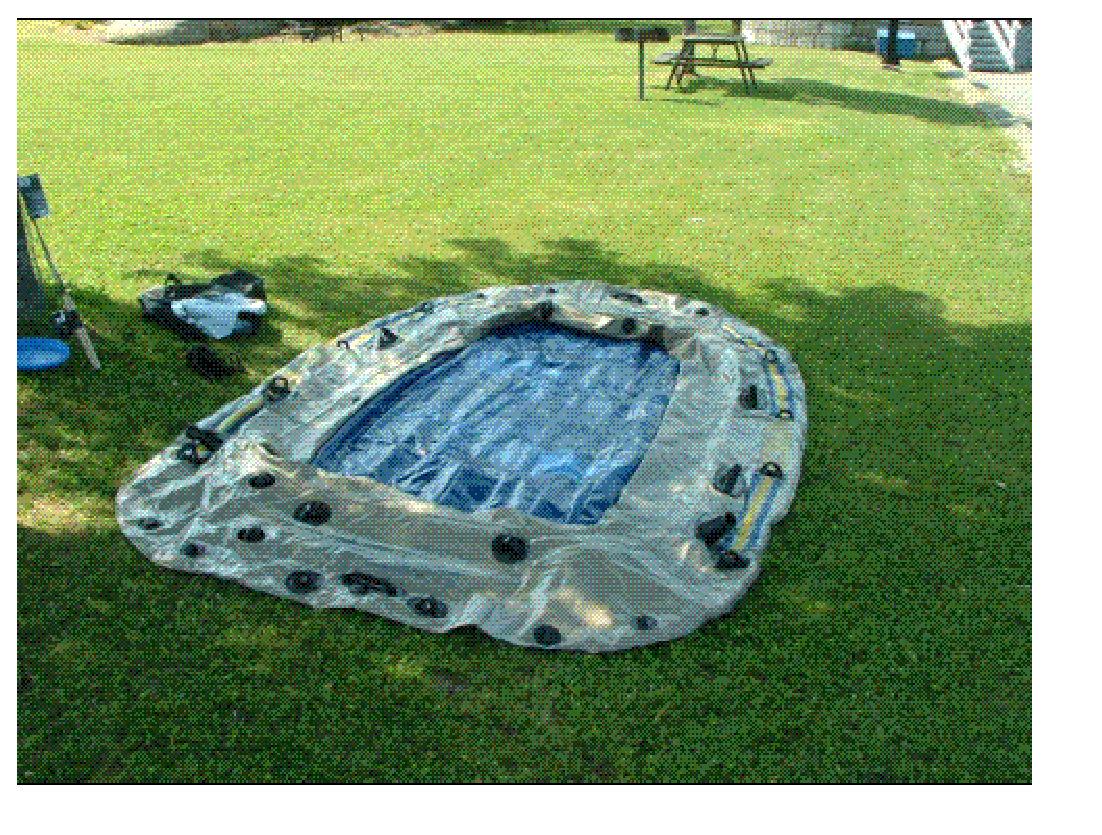
\epsfig{file=fig1.eps,width=3.5in}
Which one of the following is missing in it?
  
  
\noindent\hspace{3.0in} \begin{tabular}{|l|}
\hline
Your choice \\
\hline
 \\ 
 \\ 
\hline
\end{tabular}
  
  
 
 
\noindent{\textbf{\large{
A.}}}
An air-boat
 
 
\noindent{\textbf{\large{
B.}}}
Lawn
 
 
\noindent{\textbf{\large{
C.}}}
A frisbee
 
 
\noindent{\textbf{\large{
D.}}}
A table
 
 
\noindent{\textbf{\large{
E.}}}
A truck
 
 
\noindent{\textbf{\large{
F.}}}
  Not any of aboves.
 
 
 
\vspace{0.3in}
  
\vspace{0.2in}
  
         \begin{tabular}{|l|}
\hline
 Your marks  \\
\hline
 \\ 
 \\ 
\hline
\end{tabular}
\hspace{0.05in} \begin{tabular}{|l|}
\hline
 Full marks  \\
\hline
 \\ 
12.50 \\
\hline
\end{tabular}
{\textbf{\Large{Question
27.1.3 
}}}
  
  
 
An object is subjected to an external net force $\mathbf{f}=(
30.0 ,
6.0,
-6000.0  )N$. Its mass is known as
$m= % 
56.0  kg$. Please choose the correct accelaration
from the following choices.
 
  
  
\noindent\hspace{3.0in} \begin{tabular}{|l|}
\hline
Your choice \\
\hline
 \\ 
 \\ 
\hline
\end{tabular}
  
  
 
 
\noindent{\textbf{\large{
A.}}}
The accelaration (vector) is
$(
33534.,
1388.6 ,
4.0588 \times 10^{6}
)km/h^2.
$
 
 
\noindent{\textbf{\large{
B.}}}
The accelaration (vector) is
$(
33534.,
1388.6 ,
-1.3886 \times 10^{6}
)km/h^2.
$
 
 
\noindent{\textbf{\large{
C.}}}
The accelaration (vector) is
$(
31572.,
1388.6 ,
5.1924 \times 10^{6}
)km/h^2.
$
 
 
\noindent{\textbf{\large{
D.}}}
The accelaration (vector) is
$(
31572.,
1388.6 ,
4.0588 \times 10^{6}
)km/h^2.
$
 
 
\noindent{\textbf{\large{
E.}}}
The accelaration (vector) is
$(
33534.,
1388.6 ,
-4.2089 \times 10^{6}
)km/h^2.
$
 
 
\noindent{\textbf{\large{
F.}}}
The accelaration (vector) is
$(
32936.,
1388.6 ,
-1.3886 \times 10^{6}
)km/h^2.
$
 
 
\noindent{\textbf{\large{
G.}}}
The accelaration (vector) is
$(
32936.,
1388.6 ,
5.1924 \times 10^{6}
)km/h^2.
$
 
 
\noindent{\textbf{\large{
H.}}}
The accelaration (vector) is
$(
6942.9,
1388.6 ,
4.0588 \times 10^{6}
)km/h^2.
$
 
 
\noindent{\textbf{\large{
I.}}}
The accelaration (vector) is
$(
6942.9,
1388.6 ,
-4.2089 \times 10^{6}
)km/h^2.
$
 
 
\noindent{\textbf{\large{
J.}}}
The accelaration (vector) is
$(
33534.,
1388.6 ,
5.1924 \times 10^{6}
)km/h^2.
$
 
 
\noindent{\textbf{\large{
K.}}}
The accelaration (vector) is
$(
6942.9,
1388.6 ,
-1.3886 \times 10^{6}
)km/h^2.
$
 
 
\noindent{\textbf{\large{
L.}}}
The accelaration (vector) is
$(
32936.,
1388.6 ,
4.0588 \times 10^{6}
)km/h^2.
$
 
 
 
 

 
 
\vspace{0.3in}
  
\vspace{0.2in}
  
         \begin{tabular}{|l|}
\hline
 Your marks  \\
\hline
 \\ 
 \\ 
\hline
\end{tabular}
\hspace{0.05in} \begin{tabular}{|l|}
\hline
 Full marks  \\
\hline
 \\ 
12.50 \\
\hline
\end{tabular}
{\textbf{\Large{Question
27.1.4 
}}}
  
  
 
An object is subjected to an external net force $\mathbf{f}=(
20.0 ,
6.0,
-3000.0  )N$. Its mass is known as
$m= % 
52.0  kg$. Please choose the correct accelaration
from the following choices.
 
  
  
\noindent\hspace{3.0in} \begin{tabular}{|l|}
\hline
Your choice \\
\hline
 \\ 
 \\ 
\hline
\end{tabular}
  
  
 
 
\noindent{\textbf{\large{
A.}}}
The accelaration is
$(
-1.3940ms^{-2},
0.11538ms^{-2},
1.7163 \times 10^{6}km/h^2
).
$
 
 
\noindent{\textbf{\large{
B.}}}
The accelaration is
$(
-1.3940ms^{-2},
0.50998ms^{-2},
1.7163 \times 10^{6}km/h^2
).
$
 
 
\noindent{\textbf{\large{
C.}}}
The accelaration is
$(
0.38462ms^{-2},
0.11538ms^{-2},
-747692.km/h^2
).
$
 
 
\noindent{\textbf{\large{
D.}}}
The accelaration is
$(
0.38462ms^{-2},
0.50998ms^{-2},
1.7163 \times 10^{6}km/h^2
).
$
 
 
\noindent{\textbf{\large{
E.}}}
none of these.
 
 
 
 

 
\vspace{0.3in}
  
\vspace{0.2in}
  
         \begin{tabular}{|l|}
\hline
 Your marks  \\
\hline
 \\ 
 \\ 
\hline
\end{tabular}
\hspace{0.05in} \begin{tabular}{|l|}
\hline
 Full marks  \\
\hline
 \\ 
12.50 \\
\hline
\end{tabular}
{\textbf{\Large{Question
27.1.5 
}}}
  
  
What is the operation between $a= % 
7$ and $b= % 
6$:
$a$  % 
$\times$ $b=?$ Please also calculate it.

 
\vspace{0.3in}
  
\vspace{0.2in}
  
         \begin{tabular}{|l|}
\hline
 Your marks  \\
\hline
 \\ 
 \\ 
\hline
\end{tabular}
\hspace{0.05in} \begin{tabular}{|l|}
\hline
 Full marks  \\
\hline
 \\ 
12.50 \\
\hline
\end{tabular}
{\textbf{\Large{Question
27.1.6 
}}}
  
  
In a hotel, the possiblity of  % 
non-smoking customer is
$a =  % 
7.0 \times 10^{-2}$, and the possiblity of  % 
equal or above 30 years old customer is $ b =  % 
0.6800$.
Please calculate the possiblity of  % 
smoking and  % 
under 30 years old customer.
 

 

 
\vspace{0.3in}
   
   
\vspace{0.3in}
{\textbf{\LARGE{You have done all the above? A very good beginning, please go ahead.}}}
More constants the
Mass of electron
$m_e$$ =
9.109390 \times 10^{-31} $
kg
,
Universal gas constant
$R$$ =
8.315 $
J/(mol$\cdot $K)
,
$e$$ =
1.60217733 \times 10^{-19} $
C
, and
$m_p$$ =
1.6726231 \times 10^{-27} $
kg
%
may be very helpful.
\vspace{0.3in}
   
   
  
\vspace{0.2in}
  
\noindent\begin{tabular}{|l|}
\hline
 YOUR MARKS  \\
\hline
 \\ 
 \\ 
\hline
\end{tabular}
\hspace{0.05in} \begin{tabular}{|l|}
\hline
 Full Marks  \\
\hline
 \\ 
3.12 \\
\hline
\end{tabular}
{\textbf{\Large{QUESTION
27.2 
}}}
  
  
 
 
An object is subjected to an external net force $\mathbf{f}=
(40.0 , 9.0 , -7000.0) N$.
Its mass is known as $m= % 
58.0000 kg$. Please choose the
correct accelaration from the following choices.
 
  
  
\noindent\hspace{3.0in} \begin{tabular}{|l|}
\hline
Your choice \\
\hline
 \\ 
 \\ 
\hline
\end{tabular}
  
  
 
 
\noindent{\textbf{\large{
A.}}}
The accelaration is $  %
(
0.690,
0.16,
-120.69)
ms^{-2} $.
 
 
\noindent{\textbf{\large{
B.}}}
The accelaration is $  %
(
-2.04,
0.46,
576.39)
ms^{-2} $.
 
 
\noindent{\textbf{\large{
C.}}}
The accelaration is $  %
(
-2.04,
0.46,
-120.69)
ms^{-2} $.
 
 
\noindent{\textbf{\large{
D.}}}
The accelaration is $  %
(
0.690,
0.46,
-120.69)
ms^{-2} $.
 
 
\noindent{\textbf{\large{
E.}}}
The accelaration is $  %
(
-2.04,
0.16,
-120.69)
ms^{-2} $.
 
 
\noindent{\textbf{\large{
F.}}}
The accelaration is $  %
(
0.690,
0.46,
576.39)
ms^{-2} $.
 
 
\noindent{\textbf{\large{
G.}}}
The accelaration is $  %
(
0.690,
0.16,
576.39)
ms^{-2} $.
 
 
\noindent{\textbf{\large{
H.}}}
The accelaration is $  %
(
-2.04,
0.16,
576.39)
ms^{-2} $.
 
 
 

 

 
\vspace{0.3in}
  
\vspace{0.2in}
  
\noindent\begin{tabular}{|l|}
\hline
 YOUR MARKS  \\
\hline
 \\ 
 \\ 
\hline
\end{tabular}
\hspace{0.05in} \begin{tabular}{|l|}
\hline
 Full Marks  \\
\hline
 \\ 
1.56 \\
\hline
\end{tabular}
{\textbf{\Large{QUESTION
27.3 
}}}
  
  
Please choose the correct one from the following statements:
  
  
\noindent\hspace{3.0in} \begin{tabular}{|l|}
\hline
Your choice \\
\hline
 \\ 
 \\ 
\hline
\end{tabular}
  
  
 
 
\noindent{\textbf{\large{
A.}}}
Canada has  %
35 provinces and  %
34 territories.
 
 
\noindent{\textbf{\large{
B.}}}
Canada has  %
37 provinces and  %
37 territories.
 
 
\noindent{\textbf{\large{
C.}}}
Canada has  %
34 provinces and  %
39 territories.
 
 
\noindent{\textbf{\large{
D.}}}
Canada has  %
33 provinces and  %
38 territories.
 
 
\noindent{\textbf{\large{
E.}}}
Canada has  %
10 provinces and  %
3 territories.
 
 
\noindent{\textbf{\large{
F.}}}
 None of above.
 
 
  
\vspace{0.2in}
  
\noindent\begin{tabular}{|l|}
\hline
 YOUR MARKS  \\
\hline
 \\ 
 \\ 
\hline
\end{tabular}
\hspace{0.05in} \begin{tabular}{|l|}
\hline
 Full Marks  \\
\hline
 \\ 
1.56 \\
\hline
\end{tabular}
{\textbf{\Large{QUESTION
27.4 
}}}
  
  
 
An object is subjected to an external net force $\mathbf{f}=(
40.000 ,
3.0000,
-3000.0  )N$. Its mass is known as
$m= % 
54.0000  kg$. Please choose the correct accelaration
from the following choices.
 
  
  
\noindent\hspace{3.0in} \begin{tabular}{|l|}
\hline
Your choice \\
\hline
 \\ 
 \\ 
\hline
\end{tabular}
  
  
 
 
\noindent{\textbf{\large{
A.}}}
The accelaration is
$(
0.74074ms^{-2},
720.00km/h^2,
-55.556ms^{-2}
).
$
 
 
\noindent{\textbf{\large{
B.}}}
The accelaration is
$(
3.0767ms^{-2},
720.00km/h^2,
237.05ms^{-2}
).
$
 
 
\noindent{\textbf{\large{
C.}}}
The accelaration is
$(
3.0767ms^{-2},
3596.1km/h^2,
-55.556ms^{-2}
).
$
 
 
\noindent{\textbf{\large{
D.}}}
The accelaration is
$(
0.74074ms^{-2},
3596.1km/h^2,
237.05ms^{-2}
).
$
 
 
\noindent{\textbf{\large{
E.}}}
The accelaration is
$(
0.74074ms^{-2},
3596.1km/h^2,
-55.556ms^{-2}
).
$
 
 
\noindent{\textbf{\large{
F.}}}
The accelaration is
$(
3.0767ms^{-2},
720.00km/h^2,
-55.556ms^{-2}
).
$
 
 
\noindent{\textbf{\large{
G.}}}
 None of these.
 
 
 
 

 
\vspace{0.3in}
  
\vspace{0.2in}
  
\noindent\begin{tabular}{|l|}
\hline
 YOUR MARKS  \\
\hline
 \\ 
 \\ 
\hline
\end{tabular}
\hspace{0.05in} \begin{tabular}{|l|}
\hline
 Full Marks  \\
\hline
 \\ 
3.12 \\
\hline
\end{tabular}
{\textbf{\Large{QUESTION
27.5 
}}}
  
  
Considering case-insensitivity, please match the following same strings.
  
  
\begin{tabular}{|l|l|l|}
 \hline
 Column Left & Column Right  & Your choinces \\ 
 \hline
{\textbf{\large{
A.}}}
C
  & 
eR
 & 
 \\ 
 \hline
{\textbf{\large{
B.}}}
 A= %
2/ %
2

  & 
 a= %
1
 & 
 \\ 
 \hline
{\textbf{\large{
C.}}}
yjh
  & 
ER
 & 
 \\ 
 \hline
{\textbf{\large{
D.}}}
Er
  & 
YJH
 & 
 \\ 
 \hline
{\textbf{\large{
E.}}}
er
  & 
c
 & 
 \\ 
 \hline
 \end{tabular}
  
  
 
  
\vspace{0.2in}
  
\noindent\begin{tabular}{|l|}
\hline
 YOUR MARKS  \\
\hline
 \\ 
 \\ 
\hline
\end{tabular}
\hspace{0.05in} \begin{tabular}{|l|}
\hline
 Full Marks  \\
\hline
 \\ 
1.56 \\
\hline
\end{tabular}
{\textbf{\Large{QUESTION
27.6 
}}}
  
  
If any one of the following statements is correct, please fill the box ahead of it with $T$ .
If wrong, fill with $F$.
 
\noindent\begin{tabular}{|l|l|}\hline Your&\hspace{.2in} \\ answer&\hspace{.2in} \\ \hline \end{tabular}
1. $ % 
22$ is an  % 
odd number.
 
\noindent\begin{tabular}{|l|l|}\hline Your&\hspace{.2in} \\ answer&\hspace{.2in} \\ \hline \end{tabular}
2.  % 
Toronto is in  % 
Ontario province.
 
\noindent\begin{tabular}{|l|l|}\hline Your&\hspace{.2in} \\ answer&\hspace{.2in} \\ \hline \end{tabular}
3.  % 
$\mathbf{F}=m\mathbf{a}$ is a mathmatical form of
the Newton's Second Law.
 

 
\vspace{0.3in}
   
   
\vspace{0.3in}
{\textbf{\LARGE{You have done all the above? Excellent! Not much left, please continue.}}}
\vspace{0.3in}
   
   
  
\vspace{0.2in}
  
\noindent\begin{tabular}{|l|}
\hline
 YOUR MARKS  \\
\hline
 \\ 
 \\ 
\hline
\end{tabular}
\hspace{0.05in} \begin{tabular}{|l|}
\hline
 Full Marks  \\
\hline
 \\ 
12.50 \\
\hline
\end{tabular}
{\textbf{\Large{QUESTION
27.7 
}}}
  
  
 
$ \left( \begin{array}{ccccccccc}
           5  & 
           4  & 
           5  & 
           4  \\ 
           5  & 
           6  & 
           5  & 
           6  \\ 
           5  & 
           6  & 
           6  & 
           5
\end{array}\right) \times
\left( \begin{array}{c}
           2  \\ 
           2  \\ 
           2  \\ 
           2
\end{array}\right) $ =?
 
 
$  % 
 \left( \begin{array}
 {
 c
 c
 }
 \Phi & 
 \Phi \\ 
 \Gamma & 
 \alpha \\ 
 \varepsilon & 
 \Gamma \\ 
 \alpha & 
 \sigma
 \end{array} \right)
 \left( \begin{array}
 {
 c
 }
 \beta \\ 
 \beta
 \end{array} \right)
$ =?
 

 

 
\vspace{0.3in}
  
\vspace{0.2in}
  
\noindent\begin{tabular}{|l|}
\hline
 YOUR MARKS  \\
\hline
 \\ 
 \\ 
\hline
\end{tabular}
\hspace{0.05in} \begin{tabular}{|l|}
\hline
 Full Marks  \\
\hline
 \\ 
12.50 \\
\hline
\end{tabular}
{\textbf{\Large{QUESTION
27.8 
}}}
  
  
 
An object is subjected to an external net force $\mathbf{f}=
(70.0 , 6.0 , -6000.0) N$.
Its mass is known as $m= % 
56.0 kg$.
Please choose the correct accelaration from the following choices.
  
  
\noindent\hspace{3.0in} \begin{tabular}{|l|}
\hline
Your choice \\
\hline
 \\ 
 \\ 
\hline
\end{tabular}
  
  
 
 
\noindent{\textbf{\large{
A.}}}
  The accelaration is $  %
(
1.25,
0.39,
-404.27)
ms^{-2} $.
 
 
\noindent{\textbf{\large{
B.}}}
  The accelaration is $  %
(
1.25,
0.11,
-107.14)
ms^{-2} $.
 
 
\noindent{\textbf{\large{
C.}}}
  The accelaration is $  %
(
-3.60,
0.11,
-107.14)
ms^{-2} $.
 
 
\noindent{\textbf{\large{
D.}}}
  The accelaration is $  %
(
-3.60,
0.11,
-404.27)
ms^{-2} $.
 
 
 

 
 
\vspace{0.3in}
  
\vspace{0.2in}
  
\noindent\begin{tabular}{|l|}
\hline
 YOUR MARKS  \\
\hline
 \\ 
 \\ 
\hline
\end{tabular}
\hspace{0.05in} \begin{tabular}{|l|}
\hline
 Full Marks  \\
\hline
 \\ 
1.56 \\
\hline
\end{tabular}
{\textbf{\Large{QUESTION
27.9 
}}}
  
  
 
 
% First root
% Second root

 
Please solve the following equation:
\begin{eqnarray*}
7 \times x^2  % 
-252
                 \times x    % 
+  % 
1925 =0
\end{eqnarray*}
 

 

 
\vspace{0.3in}
   
   
 \vspace{0.2in}
Here are still some constants for use:
 
 
\noindent\begin{tabular}{|l|l|l|}
\hline
Constant & Symbol & Value \\
\hline
 
Mass of proton &
$m_p$ &
 $ 1.6726231 \times 10^{-27} $
kg \\
\hline
 
Boltzmann's constant &
$k$ &
 $ 1.381 \times 10^{-23} $
J/K \\
\hline
 
\end{tabular}
 
Thank you very much for answering these questions!
 
{\textbf{\large{Please be advised}}} that in this paper there are questions from
27.1 through
27.9.
And any one of them may contain more than one sub-question, thus the total number
of sub-questions here is around 14, of which
13 should be answered.
 
   
   
   
   
\vspace{1.0in} 
{\textbf{\large{ *** END OF PAPER, THANKS *** }}} 
   
   
\hspace{1.0in} By: 
         239 (          26 ,           34 )
   
   
   
   
\newpage 
\setcounter{page}{ 
    28001 } 
   
   
   
   
\noindent\begin{tabular}{|l|}
\hline
YOUR NAME (FIRST, ... LAST)  \\
\hline
 \\ 
 \\ 
\hline
\end{tabular}
\hspace{0.05in} \begin{tabular}{|l|}
\hline
 YOUR   ID   INFORMATION  \\
\hline
 \\ 
 \\ 
\hline
\end{tabular}
   
   
\vspace{0.2in}\noindent\begin{tabular}{|l|}
\hline
YOUR TOTAL MARKS  \\
\hline
 \\ 
 \\ 
\hline
\end{tabular}
\hspace{0.05in} \begin{tabular}{|l|}
\hline
TOTAL FULL MARKS  \\
\hline
 \\ 
100.00 \\
\hline
\end{tabular}
   
   
 \vspace{0.2in}
 
 
{\Huge  THIS IS AN EXAMPLE OF}
 
{\Huge  PERSONALIZED TESTS. }
 
If needed, please use the following constants.
 
 
 
\noindent\begin{tabular}{|l|l|l|}
\hline
Constant & Symbol & Value \\
\hline
Acceleration due to earth's gravity &
$g$ &
 $ 9.80 $
m/s$^2$ \\
\hline
Avogadro's number &
$N_A$ &
 $ 6.0221367 \times 10^{23} $
mol$^{-1}$ \\
\hline
Boltzmann's constant &
$k$ &
 $ 1.380658 \times 10^{-23} $
J/K \\
\hline
Coulomb's constant &
$k$ &
 $ 8.99 \times 10^{9} $
N$\cdot $m$^2$/C$^2$ \\
\hline
Electron charge magnitiude &
$e$ &
 $ 1.60217733 \times 10^{-19} $
C \\
\hline
Permeability of free space &
$\mu _0$ &
 $ 1.25663706 \times 10^{-6} $
T$\cdot $m/A \\
\hline
Permittivity of free space &
$\epsilon _0$ &
 $ 8.854187817 \times 10^{-12} $
C$^2$/(N$\cdot $m$^2$) \\
\hline
Pi &
$\pi$ &
 $ 3.14159265 $
$ $ \\
\hline
Planck's constant &
$h$ &
 $ 6.6260755 \times 10^{-34} $
J$\cdot $s \\
\hline
Mass of electron &
$m_e$ &
 $ 9.1093897 \times 10^{-31} $
kg \\
\hline
\end{tabular}
 
 
\noindent\begin{tabular}{|l|l|l|}
\hline
Constant & Symbol & Value \\
\hline
Mass of neutron &
$m_n$ &
 $ 1.6749286 \times 10^{-27} $
kg \\
\hline
Mass of proton &
$m_p$ &
 $ 1.6726231 \times 10^{-27} $
kg \\
\hline
Speed of light in vacuum &
$c$ &
 $ 299792458. $
m/s \\
\hline
Universal gravitational constant &
$G$ &
 $ 6.67259 \times 10^{-11} $
N$\cdot $m$^2$/kg$^2$ \\
\hline
Universal gas constant &
$R$ &
 $ 8.314510 $
J/(mol$\cdot $K) \\
\hline
\end{tabular}
 
 
{\textbf{\large{Please be advised}}} that in this paper there are questions from
28.1 through
28.9.
And any one of them may contain more than one sub-question, thus the total number
of sub-questions here is around 14, of which
13 should be answered.
 
\vspace{0.3in}
 
 
   
   
  
\vspace{0.2in}
  
\noindent\begin{tabular}{|l|}
\hline
 YOUR MARKS  \\
\hline
 \\ 
 \\ 
\hline
\end{tabular}
\hspace{0.05in} \begin{tabular}{|l|}
\hline
 Full Marks  \\
\hline
 \\ 
62.50 \\
\hline
\end{tabular}
{\textbf{\Large{QUESTION
28.1 
}}}
  
  
 
{\textbf{\Large{Please answer ONLY
5 of the following
6 questions (Questions
28.1.1 through
28.1.6). }}}
 
Here are still some constants for use in the following questions:
 
 
\noindent\begin{tabular}{|l|l|l|}
\hline
Constant & Symbol & Value \\
\hline
 
Boltzmann's constant &
$k$ &
 $ 1.381 \times 10^{-23} $
J/K \\
\hline
 
Avogadro's number &
$N_A$ &
 $ 6.022 \times 10^{23} $
mol$^{-1}$ \\
\hline
 
Mass of electron &
$m_e$ &
 $ 9.1093897 \times 10^{-31} $
kg \\
\hline
 
\end{tabular}
 
  
\vspace{0.2in}
  
         \begin{tabular}{|l|}
\hline
 Your marks  \\
\hline
 \\ 
 \\ 
\hline
\end{tabular}
\hspace{0.05in} \begin{tabular}{|l|}
\hline
 Full marks  \\
\hline
 \\ 
12.50 \\
\hline
\end{tabular}
{\textbf{\Large{Question
28.1.1 
}}}
  
  
 
An object is subjected to an external net force $\mathbf{f}=(
80.0 ,
6.0,
-7000.0  )N$. Its mass is known as
$m= % 
58.0  kg$. Please choose the correct accelaration
from the following choices.
 
  
  
\noindent\hspace{3.0in} \begin{tabular}{|l|}
\hline
Your choice \\
\hline
 \\ 
 \\ 
\hline
\end{tabular}
  
  
 
 
\noindent{\textbf{\large{
A.}}}
The accelaration is
$(
1.3793ms^{-2},
0.44087ms^{-2},
-6.5340 \times 10^{6}km/h^2
).
$
 
 
\noindent{\textbf{\large{
B.}}}
The accelaration is
$(
1.3793ms^{-2},
0.44087ms^{-2},
-1.5641 \times 10^{6}km/h^2
).
$
 
 
\noindent{\textbf{\large{
C.}}}
The accelaration is
$(
6.0670ms^{-2},
0.10345ms^{-2},
-1.5641 \times 10^{6}km/h^2
).
$
 
 
\noindent{\textbf{\large{
D.}}}
The accelaration is
$(
6.0670ms^{-2},
0.44087ms^{-2},
-6.5340 \times 10^{6}km/h^2
).
$
 
 
\noindent{\textbf{\large{
E.}}}
none of these.
 
 
 
 

 
\vspace{0.3in}
  
\vspace{0.2in}
  
         \begin{tabular}{|l|}
\hline
 Your marks  \\
\hline
 \\ 
 \\ 
\hline
\end{tabular}
\hspace{0.05in} \begin{tabular}{|l|}
\hline
 Full marks  \\
\hline
 \\ 
12.50 \\
\hline
\end{tabular}
{\textbf{\Large{Question
28.1.2 
}}}
  
  
 
An object is subjected to an external net force $\mathbf{f}=(
30.0 ,
2.0,
-9000.0  )N$. Its mass is known as
$m= % 
54.0  kg$. Please choose the correct accelaration
from the following choices.
 
  
  
\noindent\hspace{3.0in} \begin{tabular}{|l|}
\hline
Your choice \\
\hline
 \\ 
 \\ 
\hline
\end{tabular}
  
  
 
 
\noindent{\textbf{\large{
A.}}}
The accelaration (vector) is
$(
30346.,
480.00 ,
7.4382 \times 10^{6}
)km/h^2.
$
 
 
\noindent{\textbf{\large{
B.}}}
The accelaration (vector) is
$(
33869.,
480.00 ,
7.4382 \times 10^{6}
)km/h^2.
$
 
 
\noindent{\textbf{\large{
C.}}}
The accelaration (vector) is
$(
30346.,
480.00 ,
8.5317 \times 10^{6}
)km/h^2.
$
 
 
\noindent{\textbf{\large{
D.}}}
The accelaration (vector) is
$(
33869.,
480.00 ,
-2.1600 \times 10^{6}
)km/h^2.
$
 
 
\noindent{\textbf{\large{
E.}}}
The accelaration (vector) is
$(
35630.,
480.00 ,
-2.1600 \times 10^{6}
)km/h^2.
$
 
 
\noindent{\textbf{\large{
F.}}}
The accelaration (vector) is
$(
7200.0,
480.00 ,
7.4382 \times 10^{6}
)km/h^2.
$
 
 
\noindent{\textbf{\large{
G.}}}
The accelaration (vector) is
$(
7200.0,
480.00 ,
7.2656 \times 10^{6}
)km/h^2.
$
 
 
\noindent{\textbf{\large{
H.}}}
The accelaration (vector) is
$(
7200.0,
480.00 ,
-2.1600 \times 10^{6}
)km/h^2.
$
 
 
\noindent{\textbf{\large{
I.}}}
The accelaration (vector) is
$(
30346.,
480.00 ,
7.2656 \times 10^{6}
)km/h^2.
$
 
 
\noindent{\textbf{\large{
J.}}}
The accelaration (vector) is
$(
35630.,
480.00 ,
8.5317 \times 10^{6}
)km/h^2.
$
 
 
\noindent{\textbf{\large{
K.}}}
The accelaration (vector) is
$(
33869.,
480.00 ,
8.5317 \times 10^{6}
)km/h^2.
$
 
 
\noindent{\textbf{\large{
L.}}}
The accelaration (vector) is
$(
7200.0,
480.00 ,
8.5317 \times 10^{6}
)km/h^2.
$
 
 
 
 

 
 
\vspace{0.3in}
  
\vspace{0.2in}
  
         \begin{tabular}{|l|}
\hline
 Your marks  \\
\hline
 \\ 
 \\ 
\hline
\end{tabular}
\hspace{0.05in} \begin{tabular}{|l|}
\hline
 Full marks  \\
\hline
 \\ 
12.50 \\
\hline
\end{tabular}
{\textbf{\Large{Question
28.1.3 
}}}
  
  
 
An object is subjected to an external net force $\mathbf{f}=(
50.0,  % 
4.0,
-6000.0  )N$. Its mass is known as
$m= % 
58.0 kg$. Please calculate its accelaration.
 
 

 

 
\vspace{0.3in}
  
\vspace{0.2in}
  
         \begin{tabular}{|l|}
\hline
 Your marks  \\
\hline
 \\ 
 \\ 
\hline
\end{tabular}
\hspace{0.05in} \begin{tabular}{|l|}
\hline
 Full marks  \\
\hline
 \\ 
12.50 \\
\hline
\end{tabular}
{\textbf{\Large{Question
28.1.4 
}}}
  
  
What is the operation between $a= % 
5$ and $b= % 
8$:
$a$  % 
$-$ $b=?$ Please also calculate it.

 
\vspace{0.3in}
  
\vspace{0.2in}
  
         \begin{tabular}{|l|}
\hline
 Your marks  \\
\hline
 \\ 
 \\ 
\hline
\end{tabular}
\hspace{0.05in} \begin{tabular}{|l|}
\hline
 Full marks  \\
\hline
 \\ 
12.50 \\
\hline
\end{tabular}
{\textbf{\Large{Question
28.1.5 
}}}
  
  
In a hotel, the possiblity of  % 
smoking customer is
$a =  % 
0.600$, and the possiblity of  % 
equal or above 30 years old customer is $ b =  % 
0.9800$.
Please calculate the possiblity of  % 
 non-smoking and  % 
under 30 years old customer.
 

 

 
\vspace{0.3in}
  
\vspace{0.2in}
  
         \begin{tabular}{|l|}
\hline
 Your marks  \\
\hline
 \\ 
 \\ 
\hline
\end{tabular}
\hspace{0.05in} \begin{tabular}{|l|}
\hline
 Full marks  \\
\hline
 \\ 
12.50 \\
\hline
\end{tabular}
{\textbf{\Large{Question
28.1.6 
}}}
  
  
In a hotel, the possiblity of  % 
non-smoking customer is
$a =  % 
0.770$, and the possiblity of  % 
equal-or-above 30 years old customer is $ b =  % 
0.1400$.
Please fill the following form.
 
\noindent
\begin{tabular}{|l|l|}
\hline
Customer & Possibility \\
\hline
smoking  and   % 
equal-or-above 30 years old  & \\
\hline
smoking  and   % 
under 30 years old & \\
\hline
 non-smoking and   % 
equal-or-above 30 years old  & \\
\hline
 non-smoking and  % 
under 30 years old & \\
\hline
\end{tabular}
 
 
 

 

 
\vspace{0.3in}
   
   
\vspace{0.3in}
{\textbf{\LARGE{You have done all the above? A very good beginning, please go ahead.}}}
More constants the
Mass of electron
$m_e$$ =
9.109390 \times 10^{-31} $
kg
,
Universal gas constant
$R$$ =
8.315 $
J/(mol$\cdot $K)
,
$e$$ =
1.60217733 \times 10^{-19} $
C
, and
$m_p$$ =
1.6726231 \times 10^{-27} $
kg
%
may be very helpful.
\vspace{0.3in}
   
   
  
\vspace{0.2in}
  
\noindent\begin{tabular}{|l|}
\hline
 YOUR MARKS  \\
\hline
 \\ 
 \\ 
\hline
\end{tabular}
\hspace{0.05in} \begin{tabular}{|l|}
\hline
 Full Marks  \\
\hline
 \\ 
1.56 \\
\hline
\end{tabular}
{\textbf{\Large{QUESTION
28.2 
}}}
  
  
If any one of the following statements is correct, please fill the box ahead of it with $T$ .
If wrong, fill with $F$.
 
\noindent\begin{tabular}{|l|l|}\hline Your&\hspace{.2in} \\ answer&\hspace{.2in} \\ \hline \end{tabular}
1. $ % 
53$ is an  % 
even number.
 
\noindent\begin{tabular}{|l|l|}\hline Your&\hspace{.2in} \\ answer&\hspace{.2in} \\ \hline \end{tabular}
2.  % 
Kingston is in  % 
Ontario province.
 
\noindent\begin{tabular}{|l|l|}\hline Your&\hspace{.2in} \\ answer&\hspace{.2in} \\ \hline \end{tabular}
3.  % 
$\left| \mathbf{F}\right| =Gm_1m_2r^{-2}$ is a mathmatical form of
the Newton's Second Law.
 

 
\vspace{0.3in}
  
\vspace{0.2in}
  
\noindent\begin{tabular}{|l|}
\hline
 YOUR MARKS  \\
\hline
 \\ 
 \\ 
\hline
\end{tabular}
\hspace{0.05in} \begin{tabular}{|l|}
\hline
 Full Marks  \\
\hline
 \\ 
1.56 \\
\hline
\end{tabular}
{\textbf{\Large{QUESTION
28.3 
}}}
  
  
Please choose the correct one from the following statements:
  
  
\noindent\hspace{3.0in} \begin{tabular}{|l|}
\hline
Your choice \\
\hline
 \\ 
 \\ 
\hline
\end{tabular}
  
  
 
 
\noindent{\textbf{\large{
A.}}}
Canada has  %
34 provinces and  %
39 territories.
 
 
\noindent{\textbf{\large{
B.}}}
Canada has  %
37 provinces and  %
37 territories.
 
 
\noindent{\textbf{\large{
C.}}}
Canada has  %
33 provinces and  %
38 territories.
 
 
\noindent{\textbf{\large{
D.}}}
Canada has  %
10 provinces and  %
3 territories.
 
 
\noindent{\textbf{\large{
E.}}}
Canada has  %
35 provinces and  %
34 territories.
 
 
\noindent{\textbf{\large{
F.}}}
 None of above.
 
 
  
\vspace{0.2in}
  
\noindent\begin{tabular}{|l|}
\hline
 YOUR MARKS  \\
\hline
 \\ 
 \\ 
\hline
\end{tabular}
\hspace{0.05in} \begin{tabular}{|l|}
\hline
 Full Marks  \\
\hline
 \\ 
1.56 \\
\hline
\end{tabular}
{\textbf{\Large{QUESTION
28.4 
}}}
  
  
 
An object is subjected to an external net force $\mathbf{f}=(
80.000 ,
7.0000,
-9000.0  )N$. Its mass is known as
$m= % 
52.0000  kg$. Please choose the correct accelaration
from the following choices.
 
  
  
\noindent\hspace{3.0in} \begin{tabular}{|l|}
\hline
Your choice \\
\hline
 \\ 
 \\ 
\hline
\end{tabular}
  
  
 
 
\noindent{\textbf{\large{
A.}}}
The accelaration is
$(
1.5385ms^{-2},
1744.6km/h^2,
461.11ms^{-2}
).
$
 
 
\noindent{\textbf{\large{
B.}}}
The accelaration is
$(
-6.2715ms^{-2},
1744.6km/h^2,
-173.08ms^{-2}
).
$
 
 
\noindent{\textbf{\large{
C.}}}
The accelaration is
$(
-6.2715ms^{-2},
-8229.0km/h^2,
-173.08ms^{-2}
).
$
 
 
\noindent{\textbf{\large{
D.}}}
The accelaration is
$(
-6.2715ms^{-2},
1744.6km/h^2,
461.11ms^{-2}
).
$
 
 
\noindent{\textbf{\large{
E.}}}
The accelaration is
$(
-6.2715ms^{-2},
-8229.0km/h^2,
461.11ms^{-2}
).
$
 
 
\noindent{\textbf{\large{
F.}}}
The accelaration is
$(
1.5385ms^{-2},
-8229.0km/h^2,
461.11ms^{-2}
).
$
 
 
\noindent{\textbf{\large{
G.}}}
 None of these.
 
 
 
 

 
\vspace{0.3in}
  
\vspace{0.2in}
  
\noindent\begin{tabular}{|l|}
\hline
 YOUR MARKS  \\
\hline
 \\ 
 \\ 
\hline
\end{tabular}
\hspace{0.05in} \begin{tabular}{|l|}
\hline
 Full Marks  \\
\hline
 \\ 
3.12 \\
\hline
\end{tabular}
{\textbf{\Large{QUESTION
28.5 
}}}
  
  
 
 
An object is subjected to an external net force $\mathbf{f}=
(80.0 , 9.0 , -7000.0) N$.
Its mass is known as $m= % 
50.0000 kg$. Please choose the
correct accelaration from the following choices.
 
  
  
\noindent\hspace{3.0in} \begin{tabular}{|l|}
\hline
Your choice \\
\hline
 \\ 
 \\ 
\hline
\end{tabular}
  
  
 
 
\noindent{\textbf{\large{
A.}}}
The accelaration is $  %
(
4.22,
0.18,
415.24)
ms^{-2} $.
 
 
\noindent{\textbf{\large{
B.}}}
The accelaration is $  %
(
4.22,
-0.54,
415.24)
ms^{-2} $.
 
 
\noindent{\textbf{\large{
C.}}}
The accelaration is $  %
(
1.60,
-0.54,
-140.00)
ms^{-2} $.
 
 
\noindent{\textbf{\large{
D.}}}
The accelaration is $  %
(
4.22,
-0.54,
-140.00)
ms^{-2} $.
 
 
\noindent{\textbf{\large{
E.}}}
The accelaration is $  %
(
1.60,
0.18,
415.24)
ms^{-2} $.
 
 
\noindent{\textbf{\large{
F.}}}
The accelaration is $  %
(
4.22,
0.18,
-140.00)
ms^{-2} $.
 
 
\noindent{\textbf{\large{
G.}}}
The accelaration is $  %
(
1.60,
0.18,
-140.00)
ms^{-2} $.
 
 
\noindent{\textbf{\large{
H.}}}
The accelaration is $  %
(
1.60,
-0.54,
415.24)
ms^{-2} $.
 
 
 

 

 
\vspace{0.3in}
  
\vspace{0.2in}
  
\noindent\begin{tabular}{|l|}
\hline
 YOUR MARKS  \\
\hline
 \\ 
 \\ 
\hline
\end{tabular}
\hspace{0.05in} \begin{tabular}{|l|}
\hline
 Full Marks  \\
\hline
 \\ 
3.12 \\
\hline
\end{tabular}
{\textbf{\Large{QUESTION
28.6 
}}}
  
  
Considering case-insensitivity, please match the following same strings.
  
  
\begin{tabular}{|l|l|l|}
 \hline
 Column Left & Column Right  & Your choinces \\ 
 \hline
{\textbf{\large{
A.}}}
C
  & 
YJH
 & 
 \\ 
 \hline
{\textbf{\large{
B.}}}
Er
  & 
eR
 & 
 \\ 
 \hline
{\textbf{\large{
C.}}}
A
  & 
ER
 & 
 \\ 
 \hline
{\textbf{\large{
D.}}}
yjh
  & 
a
 & 
 \\ 
 \hline
{\textbf{\large{
E.}}}
er
  & 
c
 & 
 \\ 
 \hline
 \end{tabular}
  
  
 
   
   
\vspace{0.3in}
{\textbf{\LARGE{You have done all the above? Excellent! Not much left, please continue.}}}
\vspace{0.3in}
   
   
  
\vspace{0.2in}
  
\noindent\begin{tabular}{|l|}
\hline
 YOUR MARKS  \\
\hline
 \\ 
 \\ 
\hline
\end{tabular}
\hspace{0.05in} \begin{tabular}{|l|}
\hline
 Full Marks  \\
\hline
 \\ 
12.50 \\
\hline
\end{tabular}
{\textbf{\Large{QUESTION
28.7 
}}}
  
  
 
$ \left( \begin{array}{ccccccccc}
           5  & 
           5  & 
           5  & 
           7  \\ 
           4  & 
           6  & 
           6  & 
           6  \\ 
           6  & 
           6  & 
           6  & 
           5
\end{array}\right) \times
\left( \begin{array}{c}
           2  \\ 
           2  \\ 
           2  \\ 
           2
\end{array}\right) $ =?
 
 
$  % 
 \left( \begin{array}
 {
 c
 c
 }
 \eta & 
 \Phi \\ 
 \sigma & 
 \Delta \\ 
 \Psi & 
 \Psi \\ 
 \Gamma & 
 \sigma
 \end{array} \right)
 \left( \begin{array}
 {
 c
 }
 \beta \\ 
 \gamma
 \end{array} \right)
$ =?
 

 

 
\vspace{0.3in}
  
\vspace{0.2in}
  
\noindent\begin{tabular}{|l|}
\hline
 YOUR MARKS  \\
\hline
 \\ 
 \\ 
\hline
\end{tabular}
\hspace{0.05in} \begin{tabular}{|l|}
\hline
 Full Marks  \\
\hline
 \\ 
12.50 \\
\hline
\end{tabular}
{\textbf{\Large{QUESTION
28.8 
}}}
  
  
 
An object is subjected to an external net force $\mathbf{f}=
(80.0 , 6.0 , -4000.0) N$.
Its mass is known as $m= % 
56.0 kg$.
Please choose the correct accelaration from the following choices.
  
  
\noindent\hspace{3.0in} \begin{tabular}{|l|}
\hline
Your choice \\
\hline
 \\ 
 \\ 
\hline
\end{tabular}
  
  
 
 
\noindent{\textbf{\large{
A.}}}
  The accelaration is $  %
(
2.88,
0.11,
-71.429)
ms^{-2} $.
 
 
\noindent{\textbf{\large{
B.}}}
  The accelaration is $  %
(
1.43,
0.11,
251.90)
ms^{-2} $.
 
 
\noindent{\textbf{\large{
C.}}}
  The accelaration is $  %
(
1.43,
0.11,
-71.429)
ms^{-2} $.
 
 
\noindent{\textbf{\large{
D.}}}
  The accelaration is $  %
(
2.88,
-0.33,
251.90)
ms^{-2} $.
 
 
 

 
 
\vspace{0.3in}
  
\vspace{0.2in}
  
\noindent\begin{tabular}{|l|}
\hline
 YOUR MARKS  \\
\hline
 \\ 
 \\ 
\hline
\end{tabular}
\hspace{0.05in} \begin{tabular}{|l|}
\hline
 Full Marks  \\
\hline
 \\ 
1.56 \\
\hline
\end{tabular}
{\textbf{\Large{QUESTION
28.9 
}}}
  
  
 
 
% First root
% Second root

 
Please solve the following equation:
\begin{eqnarray*}
-11 \times x^2  % 
+  % 
539
                 \times x    % 
-5984 =0
\end{eqnarray*}
 

 

 
\vspace{0.3in}
   
   
 \vspace{0.2in}
Here are still some constants for use:
 
 
\noindent\begin{tabular}{|l|l|l|}
\hline
Constant & Symbol & Value \\
\hline
 
Mass of proton &
$m_p$ &
 $ 1.6726231 \times 10^{-27} $
kg \\
\hline
 
Boltzmann's constant &
$k$ &
 $ 1.381 \times 10^{-23} $
J/K \\
\hline
 
\end{tabular}
 
Thank you very much for answering these questions!
 
{\textbf{\large{Please be advised}}} that in this paper there are questions from
28.1 through
28.9.
And any one of them may contain more than one sub-question, thus the total number
of sub-questions here is around 14, of which
13 should be answered.
 
   
   
   
   
\vspace{1.0in} 
{\textbf{\large{ *** END OF PAPER, THANKS *** }}} 
   
   
\hspace{1.0in} By: 
         239 (          26 ,           34 )
   
   
   
   
\newpage 
\setcounter{page}{ 
    29001 } 
   
   
   
   
\noindent\begin{tabular}{|l|}
\hline
YOUR NAME (FIRST, ... LAST)  \\
\hline
 \\ 
 \\ 
\hline
\end{tabular}
\hspace{0.05in} \begin{tabular}{|l|}
\hline
 YOUR   ID   INFORMATION  \\
\hline
 \\ 
 \\ 
\hline
\end{tabular}
   
   
\vspace{0.2in}\noindent\begin{tabular}{|l|}
\hline
YOUR TOTAL MARKS  \\
\hline
 \\ 
 \\ 
\hline
\end{tabular}
\hspace{0.05in} \begin{tabular}{|l|}
\hline
TOTAL FULL MARKS  \\
\hline
 \\ 
100.00 \\
\hline
\end{tabular}
   
   
 \vspace{0.2in}
 
 
{\Huge  THIS IS AN EXAMPLE OF}
 
{\Huge  PERSONALIZED TESTS. }
 
If needed, please use the following constants.
 
 
 
\noindent\begin{tabular}{|l|l|l|}
\hline
Constant & Symbol & Value \\
\hline
Acceleration due to earth's gravity &
$g$ &
 $ 9.80 $
m/s$^2$ \\
\hline
Avogadro's number &
$N_A$ &
 $ 6.0221367 \times 10^{23} $
mol$^{-1}$ \\
\hline
Boltzmann's constant &
$k$ &
 $ 1.380658 \times 10^{-23} $
J/K \\
\hline
Coulomb's constant &
$k$ &
 $ 8.99 \times 10^{9} $
N$\cdot $m$^2$/C$^2$ \\
\hline
Electron charge magnitiude &
$e$ &
 $ 1.60217733 \times 10^{-19} $
C \\
\hline
Permeability of free space &
$\mu _0$ &
 $ 1.25663706 \times 10^{-6} $
T$\cdot $m/A \\
\hline
Permittivity of free space &
$\epsilon _0$ &
 $ 8.854187817 \times 10^{-12} $
C$^2$/(N$\cdot $m$^2$) \\
\hline
Pi &
$\pi$ &
 $ 3.14159265 $
$ $ \\
\hline
Planck's constant &
$h$ &
 $ 6.6260755 \times 10^{-34} $
J$\cdot $s \\
\hline
Mass of electron &
$m_e$ &
 $ 9.1093897 \times 10^{-31} $
kg \\
\hline
\end{tabular}
 
 
\noindent\begin{tabular}{|l|l|l|}
\hline
Constant & Symbol & Value \\
\hline
Mass of neutron &
$m_n$ &
 $ 1.6749286 \times 10^{-27} $
kg \\
\hline
Mass of proton &
$m_p$ &
 $ 1.6726231 \times 10^{-27} $
kg \\
\hline
Speed of light in vacuum &
$c$ &
 $ 299792458. $
m/s \\
\hline
Universal gravitational constant &
$G$ &
 $ 6.67259 \times 10^{-11} $
N$\cdot $m$^2$/kg$^2$ \\
\hline
Universal gas constant &
$R$ &
 $ 8.314510 $
J/(mol$\cdot $K) \\
\hline
\end{tabular}
 
 
{\textbf{\large{Please be advised}}} that in this paper there are questions from
29.1 through
29.9.
And any one of them may contain more than one sub-question, thus the total number
of sub-questions here is around 14, of which
13 should be answered.
 
\vspace{0.3in}
 
 
   
   
  
\vspace{0.2in}
  
\noindent\begin{tabular}{|l|}
\hline
 YOUR MARKS  \\
\hline
 \\ 
 \\ 
\hline
\end{tabular}
\hspace{0.05in} \begin{tabular}{|l|}
\hline
 Full Marks  \\
\hline
 \\ 
62.50 \\
\hline
\end{tabular}
{\textbf{\Large{QUESTION
29.1 
}}}
  
  
 
{\textbf{\Large{Please answer ONLY
5 of the following
6 questions (Questions
29.1.1 through
29.1.6). }}}
 
Here are still some constants for use in the following questions:
 
 
\noindent\begin{tabular}{|l|l|l|}
\hline
Constant & Symbol & Value \\
\hline
 
Boltzmann's constant &
$k$ &
 $ 1.381 \times 10^{-23} $
J/K \\
\hline
 
Avogadro's number &
$N_A$ &
 $ 6.022 \times 10^{23} $
mol$^{-1}$ \\
\hline
 
Mass of electron &
$m_e$ &
 $ 9.1093897 \times 10^{-31} $
kg \\
\hline
 
\end{tabular}
 
  
\vspace{0.2in}
  
         \begin{tabular}{|l|}
\hline
 Your marks  \\
\hline
 \\ 
 \\ 
\hline
\end{tabular}
\hspace{0.05in} \begin{tabular}{|l|}
\hline
 Full marks  \\
\hline
 \\ 
12.50 \\
\hline
\end{tabular}
{\textbf{\Large{Question
29.1.1 
}}}
  
  
 
An object is subjected to an external net force $\mathbf{f}=(
50.0 ,
7.0,
-5000.0  )N$. Its mass is known as
$m= % 
52.0  kg$. Please choose the correct accelaration
from the following choices.
 
  
  
\noindent\hspace{3.0in} \begin{tabular}{|l|}
\hline
Your choice \\
\hline
 \\ 
 \\ 
\hline
\end{tabular}
  
  
 
 
\noindent{\textbf{\large{
A.}}}
The accelaration (vector) is
$(
53724.,
1744.6 ,
4.2009 \times 10^{6}
)km/h^2.
$
 
 
\noindent{\textbf{\large{
B.}}}
The accelaration (vector) is
$(
53724.,
1744.6 ,
-4.5702 \times 10^{6}
)km/h^2.
$
 
 
\noindent{\textbf{\large{
C.}}}
The accelaration (vector) is
$(
56648.,
1744.6 ,
-1.2462 \times 10^{6}
)km/h^2.
$
 
 
\noindent{\textbf{\large{
D.}}}
The accelaration (vector) is
$(
12462.,
1744.6 ,
4.9047 \times 10^{6}
)km/h^2.
$
 
 
\noindent{\textbf{\large{
E.}}}
The accelaration (vector) is
$(
56648.,
1744.6 ,
4.9047 \times 10^{6}
)km/h^2.
$
 
 
\noindent{\textbf{\large{
F.}}}
The accelaration (vector) is
$(
12462.,
1744.6 ,
-1.2462 \times 10^{6}
)km/h^2.
$
 
 
\noindent{\textbf{\large{
G.}}}
The accelaration (vector) is
$(
53724.,
1744.6 ,
4.9047 \times 10^{6}
)km/h^2.
$
 
 
\noindent{\textbf{\large{
H.}}}
The accelaration (vector) is
$(
56648.,
1744.6 ,
4.2009 \times 10^{6}
)km/h^2.
$
 
 
\noindent{\textbf{\large{
I.}}}
The accelaration (vector) is
$(
50025.,
1744.6 ,
-1.2462 \times 10^{6}
)km/h^2.
$
 
 
\noindent{\textbf{\large{
J.}}}
The accelaration (vector) is
$(
56648.,
1744.6 ,
-4.5702 \times 10^{6}
)km/h^2.
$
 
 
\noindent{\textbf{\large{
K.}}}
The accelaration (vector) is
$(
12462.,
1744.6 ,
-4.5702 \times 10^{6}
)km/h^2.
$
 
 
\noindent{\textbf{\large{
L.}}}
The accelaration (vector) is
$(
50025.,
1744.6 ,
4.9047 \times 10^{6}
)km/h^2.
$
 
 
 
 

 
 
\vspace{0.3in}
  
\vspace{0.2in}
  
         \begin{tabular}{|l|}
\hline
 Your marks  \\
\hline
 \\ 
 \\ 
\hline
\end{tabular}
\hspace{0.05in} \begin{tabular}{|l|}
\hline
 Full marks  \\
\hline
 \\ 
12.50 \\
\hline
\end{tabular}
{\textbf{\Large{Question
29.1.2 
}}}
  
  
What is the operation between $a= % 
5$ and $b= % 
6$:
$a$  % 
$\times$ $b=?$ Please also calculate it.

 
\vspace{0.3in}
  
\vspace{0.2in}
  
         \begin{tabular}{|l|}
\hline
 Your marks  \\
\hline
 \\ 
 \\ 
\hline
\end{tabular}
\hspace{0.05in} \begin{tabular}{|l|}
\hline
 Full marks  \\
\hline
 \\ 
12.50 \\
\hline
\end{tabular}
{\textbf{\Large{Question
29.1.3 
}}}
  
  
In a hotel, the possiblity of  % 
smoking customer is
$a =  % 
0.230$, and the possiblity of  % 
equal-or-above 30 years old customer is $ b =  % 
0.5600$.
Please fill the following form.
 
\noindent
\begin{tabular}{|l|l|}
\hline
Customer & Possibility \\
\hline
smoking  and   % 
equal-or-above 30 years old  & \\
\hline
smoking  and   % 
under 30 years old & \\
\hline
 non-smoking and   % 
equal-or-above 30 years old  & \\
\hline
 non-smoking and  % 
under 30 years old & \\
\hline
\end{tabular}
 
 
 

 

 
\vspace{0.3in}
  
\vspace{0.2in}
  
         \begin{tabular}{|l|}
\hline
 Your marks  \\
\hline
 \\ 
 \\ 
\hline
\end{tabular}
\hspace{0.05in} \begin{tabular}{|l|}
\hline
 Full marks  \\
\hline
 \\ 
12.50 \\
\hline
\end{tabular}
{\textbf{\Large{Question
29.1.4 
}}}
  
  
 
An object is subjected to an external net force $\mathbf{f}=(
60.0,  % 
5.0,
-4000.0  )N$. Its mass is known as
$m= % 
54.0 kg$. Please calculate its accelaration.
 
 

 

 
\vspace{0.3in}
  
\vspace{0.2in}
  
         \begin{tabular}{|l|}
\hline
 Your marks  \\
\hline
 \\ 
 \\ 
\hline
\end{tabular}
\hspace{0.05in} \begin{tabular}{|l|}
\hline
 Full marks  \\
\hline
 \\ 
12.50 \\
\hline
\end{tabular}
{\textbf{\Large{Question
29.1.5 
}}}
  
  
 
An object is subjected to an external net force $\mathbf{f}=(
60.0 ,
6.0,
-3000.0  )N$. Its mass is known as
$m= % 
54.0  kg$. Please choose the correct accelaration
from the following choices.
 
  
  
\noindent\hspace{3.0in} \begin{tabular}{|l|}
\hline
Your choice \\
\hline
 \\ 
 \\ 
\hline
\end{tabular}
  
  
 
 
\noindent{\textbf{\large{
A.}}}
The accelaration is
$(
1.1111ms^{-2},
0.42695ms^{-2},
-2.1061 \times 10^{6}km/h^2
).
$
 
 
\noindent{\textbf{\large{
B.}}}
The accelaration is
$(
1.1111ms^{-2},
0.11111ms^{-2},
-2.1061 \times 10^{6}km/h^2
).
$
 
 
\noindent{\textbf{\large{
C.}}}
The accelaration is
$(
2.7139ms^{-2},
0.42695ms^{-2},
-2.1061 \times 10^{6}km/h^2
).
$
 
 
\noindent{\textbf{\large{
D.}}}
The accelaration is
$(
1.1111ms^{-2},
0.11111ms^{-2},
-720000.km/h^2
).
$
 
 
\noindent{\textbf{\large{
E.}}}
none of these.
 
 
 
 

 
\vspace{0.3in}
  
\vspace{0.2in}
  
         \begin{tabular}{|l|}
\hline
 Your marks  \\
\hline
 \\ 
 \\ 
\hline
\end{tabular}
\hspace{0.05in} \begin{tabular}{|l|}
\hline
 Full marks  \\
\hline
 \\ 
12.50 \\
\hline
\end{tabular}
{\textbf{\Large{Question
29.1.6 
}}}
  
  
In a hotel, the possiblity of  % 
smoking customer is
$a =  % 
0.770$, and the possiblity of  % 
 under 30 years old customer is $ b =  % 
0.7000$.
Please calculate the possiblity of  % 
 non-smoking and  % 
equal or above 30 years old customer.
 

 

 
\vspace{0.3in}
   
   
\vspace{0.3in}
{\textbf{\LARGE{You have done all the above? A very good beginning, please go ahead.}}}
More constants the
Mass of electron
$m_e$$ =
9.109390 \times 10^{-31} $
kg
,
Universal gas constant
$R$$ =
8.315 $
J/(mol$\cdot $K)
,
$e$$ =
1.60217733 \times 10^{-19} $
C
, and
$m_p$$ =
1.6726231 \times 10^{-27} $
kg
%
may be very helpful.
\vspace{0.3in}
   
   
  
\vspace{0.2in}
  
\noindent\begin{tabular}{|l|}
\hline
 YOUR MARKS  \\
\hline
 \\ 
 \\ 
\hline
\end{tabular}
\hspace{0.05in} \begin{tabular}{|l|}
\hline
 Full Marks  \\
\hline
 \\ 
3.12 \\
\hline
\end{tabular}
{\textbf{\Large{QUESTION
29.2 
}}}
  
  
 
 
An object is subjected to an external net force $\mathbf{f}=
(50.0 , 4.0 , -6000.0) N$.
Its mass is known as $m= % 
52.0000 kg$. Please choose the
correct accelaration from the following choices.
 
  
  
\noindent\hspace{3.0in} \begin{tabular}{|l|}
\hline
Your choice \\
\hline
 \\ 
 \\ 
\hline
\end{tabular}
  
  
 
 
\noindent{\textbf{\large{
A.}}}
The accelaration is $  %
(
0.962,
7.7 \times 10^{-2},
427.13)
ms^{-2} $.
 
 
\noindent{\textbf{\large{
B.}}}
The accelaration is $  %
(
4.16,
0.20,
-115.38)
ms^{-2} $.
 
 
\noindent{\textbf{\large{
C.}}}
The accelaration is $  %
(
4.16,
0.20,
427.13)
ms^{-2} $.
 
 
\noindent{\textbf{\large{
D.}}}
The accelaration is $  %
(
4.16,
7.7 \times 10^{-2},
-115.38)
ms^{-2} $.
 
 
\noindent{\textbf{\large{
E.}}}
The accelaration is $  %
(
0.962,
7.7 \times 10^{-2},
-115.38)
ms^{-2} $.
 
 
\noindent{\textbf{\large{
F.}}}
The accelaration is $  %
(
4.16,
7.7 \times 10^{-2},
427.13)
ms^{-2} $.
 
 
\noindent{\textbf{\large{
G.}}}
The accelaration is $  %
(
0.962,
0.20,
-115.38)
ms^{-2} $.
 
 
\noindent{\textbf{\large{
H.}}}
The accelaration is $  %
(
0.962,
0.20,
427.13)
ms^{-2} $.
 
 
 

 

 
\vspace{0.3in}
  
\vspace{0.2in}
  
\noindent\begin{tabular}{|l|}
\hline
 YOUR MARKS  \\
\hline
 \\ 
 \\ 
\hline
\end{tabular}
\hspace{0.05in} \begin{tabular}{|l|}
\hline
 Full Marks  \\
\hline
 \\ 
1.56 \\
\hline
\end{tabular}
{\textbf{\Large{QUESTION
29.3 
}}}
  
  
 
An object is subjected to an external net force $\mathbf{f}=(
50.000 ,
3.0000,
-4000.0  )N$. Its mass is known as
$m= % 
54.0000  kg$. Please choose the correct accelaration
from the following choices.
 
  
  
\noindent\hspace{3.0in} \begin{tabular}{|l|}
\hline
Your choice \\
\hline
 \\ 
 \\ 
\hline
\end{tabular}
  
  
 
 
\noindent{\textbf{\large{
A.}}}
The accelaration is
$(
0.92593ms^{-2},
720.00km/h^2,
-74.074ms^{-2}
).
$
 
 
\noindent{\textbf{\large{
B.}}}
The accelaration is
$(
4.5878ms^{-2},
-3482.9km/h^2,
-74.074ms^{-2}
).
$
 
 
\noindent{\textbf{\large{
C.}}}
The accelaration is
$(
4.5878ms^{-2},
720.00km/h^2,
346.91ms^{-2}
).
$
 
 
\noindent{\textbf{\large{
D.}}}
The accelaration is
$(
4.5878ms^{-2},
720.00km/h^2,
-74.074ms^{-2}
).
$
 
 
\noindent{\textbf{\large{
E.}}}
The accelaration is
$(
0.92593ms^{-2},
720.00km/h^2,
346.91ms^{-2}
).
$
 
 
\noindent{\textbf{\large{
F.}}}
The accelaration is
$(
0.92593ms^{-2},
-3482.9km/h^2,
346.91ms^{-2}
).
$
 
 
\noindent{\textbf{\large{
G.}}}
 None of these.
 
 
 
 

 
\vspace{0.3in}
  
\vspace{0.2in}
  
\noindent\begin{tabular}{|l|}
\hline
 YOUR MARKS  \\
\hline
 \\ 
 \\ 
\hline
\end{tabular}
\hspace{0.05in} \begin{tabular}{|l|}
\hline
 Full Marks  \\
\hline
 \\ 
3.12 \\
\hline
\end{tabular}
{\textbf{\Large{QUESTION
29.4 
}}}
  
  
Considering case-insensitivity, please match the following same strings.
  
  
\begin{tabular}{|l|l|l|}
 \hline
 Column Left & Column Right  & Your choinces \\ 
 \hline
{\textbf{\large{
A.}}}
B
  & 
ER
 & 
 \\ 
 \hline
{\textbf{\large{
B.}}}
yjh
  & 
a
 & 
 \\ 
 \hline
{\textbf{\large{
C.}}}
 A= %
4/ %
2

  & 
b
 & 
 \\ 
 \hline
{\textbf{\large{
D.}}}
A
  & 
 a= %
2
 & 
 \\ 
 \hline
{\textbf{\large{
E.}}}
er
  & 
YJH
 & 
 \\ 
 \hline
 \end{tabular}
  
  
 
  
\vspace{0.2in}
  
\noindent\begin{tabular}{|l|}
\hline
 YOUR MARKS  \\
\hline
 \\ 
 \\ 
\hline
\end{tabular}
\hspace{0.05in} \begin{tabular}{|l|}
\hline
 Full Marks  \\
\hline
 \\ 
1.56 \\
\hline
\end{tabular}
{\textbf{\Large{QUESTION
29.5 
}}}
  
  
Please choose the correct one from the following statements:
  
  
\noindent\hspace{3.0in} \begin{tabular}{|l|}
\hline
Your choice \\
\hline
 \\ 
 \\ 
\hline
\end{tabular}
  
  
 
 
\noindent{\textbf{\large{
A.}}}
Canada has  %
10 provinces and  %
3 territories.
 
 
\noindent{\textbf{\large{
B.}}}
Canada has  %
33 provinces and  %
38 territories.
 
 
\noindent{\textbf{\large{
C.}}}
Canada has  %
34 provinces and  %
39 territories.
 
 
\noindent{\textbf{\large{
D.}}}
Canada has  %
37 provinces and  %
37 territories.
 
 
\noindent{\textbf{\large{
E.}}}
Canada has  %
35 provinces and  %
34 territories.
 
 
\noindent{\textbf{\large{
F.}}}
 None of above.
 
 
  
\vspace{0.2in}
  
\noindent\begin{tabular}{|l|}
\hline
 YOUR MARKS  \\
\hline
 \\ 
 \\ 
\hline
\end{tabular}
\hspace{0.05in} \begin{tabular}{|l|}
\hline
 Full Marks  \\
\hline
 \\ 
1.56 \\
\hline
\end{tabular}
{\textbf{\Large{QUESTION
29.6 
}}}
  
  
If any one of the following statements is correct, please fill the box ahead of it with $T$ .
If wrong, fill with $F$.
 
\noindent\begin{tabular}{|l|l|}\hline Your&\hspace{.2in} \\ answer&\hspace{.2in} \\ \hline \end{tabular}
1. $ % 
69$ is an  % 
odd number.
 
\noindent\begin{tabular}{|l|l|}\hline Your&\hspace{.2in} \\ answer&\hspace{.2in} \\ \hline \end{tabular}
2.  % 
Montreal is in  % 
Ontario province.
 
\noindent\begin{tabular}{|l|l|}\hline Your&\hspace{.2in} \\ answer&\hspace{.2in} \\ \hline \end{tabular}
3.  % 
$\mathbf{F}=m\mathbf{a}$ is a mathmatical form of
the Newton's Second Law.
 

 
\vspace{0.3in}
   
   
\vspace{0.3in}
{\textbf{\LARGE{You have done all the above? Excellent! Not much left, please continue.}}}
\vspace{0.3in}
   
   
  
\vspace{0.2in}
  
\noindent\begin{tabular}{|l|}
\hline
 YOUR MARKS  \\
\hline
 \\ 
 \\ 
\hline
\end{tabular}
\hspace{0.05in} \begin{tabular}{|l|}
\hline
 Full Marks  \\
\hline
 \\ 
12.50 \\
\hline
\end{tabular}
{\textbf{\Large{QUESTION
29.7 
}}}
  
  
 
$ \left( \begin{array}{ccccccccc}
           4  & 
           5  & 
           6  & 
           6  \\ 
           6  & 
           7  & 
           4  & 
           4  \\ 
           6  & 
           5  & 
           4  & 
           6
\end{array}\right) \times
\left( \begin{array}{c}
           2  \\ 
           2  \\ 
           2  \\ 
           2
\end{array}\right) $ =?
 
 
$  % 
 \left( \begin{array}
 {
 c
 c
 }
 \delta & 
 \beta \\ 
 \Phi & 
 \Gamma \\ 
 \Delta & 
 \Psi \\ 
 \Psi & 
                    \Xi
 \end{array} \right)
 \left( \begin{array}
 {
 c
 }
 \beta \\ 
 \beta
 \end{array} \right)
$ =?
 

 

 
\vspace{0.3in}
  
\vspace{0.2in}
  
\noindent\begin{tabular}{|l|}
\hline
 YOUR MARKS  \\
\hline
 \\ 
 \\ 
\hline
\end{tabular}
\hspace{0.05in} \begin{tabular}{|l|}
\hline
 Full Marks  \\
\hline
 \\ 
12.50 \\
\hline
\end{tabular}
{\textbf{\Large{QUESTION
29.8 
}}}
  
  
 
An object is subjected to an external net force $\mathbf{f}=
(50.0 , 3.0 , -3000.0) N$.
Its mass is known as $m= % 
58.0 kg$.
Please choose the correct accelaration from the following choices.
  
  
\noindent\hspace{3.0in} \begin{tabular}{|l|}
\hline
Your choice \\
\hline
 \\ 
 \\ 
\hline
\end{tabular}
  
  
 
 
\noindent{\textbf{\large{
A.}}}
  The accelaration is $  %
(
2.38,
5.2 \times 10^{-2},
-51.724)
ms^{-2} $.
 
 
\noindent{\textbf{\large{
B.}}}
  The accelaration is $  %
(
0.862,
-0.17,
-51.724)
ms^{-2} $.
 
 
\noindent{\textbf{\large{
C.}}}
  The accelaration is $  %
(
0.862,
5.2 \times 10^{-2},
227.14)
ms^{-2} $.
 
 
\noindent{\textbf{\large{
D.}}}
  The accelaration is $  %
(
0.862,
5.2 \times 10^{-2},
-51.724)
ms^{-2} $.
 
 
 

 
 
\vspace{0.3in}
  
\vspace{0.2in}
  
\noindent\begin{tabular}{|l|}
\hline
 YOUR MARKS  \\
\hline
 \\ 
 \\ 
\hline
\end{tabular}
\hspace{0.05in} \begin{tabular}{|l|}
\hline
 Full Marks  \\
\hline
 \\ 
1.56 \\
\hline
\end{tabular}
{\textbf{\Large{QUESTION
29.9 
}}}
  
  
 
 
% First root
% Second root

 
Please solve the following equation:
\begin{eqnarray*}
11 \times x^2  % 
-671
                 \times x    % 
+  % 
10208 =0
\end{eqnarray*}
 

 

 
\vspace{0.3in}
   
   
 \vspace{0.2in}
Here are still some constants for use:
 
 
\noindent\begin{tabular}{|l|l|l|}
\hline
Constant & Symbol & Value \\
\hline
 
Mass of proton &
$m_p$ &
 $ 1.6726231 \times 10^{-27} $
kg \\
\hline
 
Boltzmann's constant &
$k$ &
 $ 1.381 \times 10^{-23} $
J/K \\
\hline
 
\end{tabular}
 
Thank you very much for answering these questions!
 
{\textbf{\large{Please be advised}}} that in this paper there are questions from
29.1 through
29.9.
And any one of them may contain more than one sub-question, thus the total number
of sub-questions here is around 14, of which
13 should be answered.
 
   
   
   
   
\vspace{1.0in} 
{\textbf{\large{ *** END OF PAPER, THANKS *** }}} 
   
   
\hspace{1.0in} By: 
         239 (          26 ,           34 )
   
   
   
   
\newpage 
\setcounter{page}{ 
    30001 } 
   
   
   
   
\noindent\begin{tabular}{|l|}
\hline
YOUR NAME (FIRST, ... LAST)  \\
\hline
 \\ 
 \\ 
\hline
\end{tabular}
\hspace{0.05in} \begin{tabular}{|l|}
\hline
 YOUR   ID   INFORMATION  \\
\hline
 \\ 
 \\ 
\hline
\end{tabular}
   
   
\vspace{0.2in}\noindent\begin{tabular}{|l|}
\hline
YOUR TOTAL MARKS  \\
\hline
 \\ 
 \\ 
\hline
\end{tabular}
\hspace{0.05in} \begin{tabular}{|l|}
\hline
TOTAL FULL MARKS  \\
\hline
 \\ 
100.00 \\
\hline
\end{tabular}
   
   
 \vspace{0.2in}
 
 
{\Huge  THIS IS AN EXAMPLE OF}
 
{\Huge  PERSONALIZED TESTS. }
 
If needed, please use the following constants.
 
 
 
\noindent\begin{tabular}{|l|l|l|}
\hline
Constant & Symbol & Value \\
\hline
Acceleration due to earth's gravity &
$g$ &
 $ 9.80 $
m/s$^2$ \\
\hline
Avogadro's number &
$N_A$ &
 $ 6.0221367 \times 10^{23} $
mol$^{-1}$ \\
\hline
Boltzmann's constant &
$k$ &
 $ 1.380658 \times 10^{-23} $
J/K \\
\hline
Coulomb's constant &
$k$ &
 $ 8.99 \times 10^{9} $
N$\cdot $m$^2$/C$^2$ \\
\hline
Electron charge magnitiude &
$e$ &
 $ 1.60217733 \times 10^{-19} $
C \\
\hline
Permeability of free space &
$\mu _0$ &
 $ 1.25663706 \times 10^{-6} $
T$\cdot $m/A \\
\hline
Permittivity of free space &
$\epsilon _0$ &
 $ 8.854187817 \times 10^{-12} $
C$^2$/(N$\cdot $m$^2$) \\
\hline
Pi &
$\pi$ &
 $ 3.14159265 $
$ $ \\
\hline
Planck's constant &
$h$ &
 $ 6.6260755 \times 10^{-34} $
J$\cdot $s \\
\hline
Mass of electron &
$m_e$ &
 $ 9.1093897 \times 10^{-31} $
kg \\
\hline
\end{tabular}
 
 
\noindent\begin{tabular}{|l|l|l|}
\hline
Constant & Symbol & Value \\
\hline
Mass of neutron &
$m_n$ &
 $ 1.6749286 \times 10^{-27} $
kg \\
\hline
Mass of proton &
$m_p$ &
 $ 1.6726231 \times 10^{-27} $
kg \\
\hline
Speed of light in vacuum &
$c$ &
 $ 299792458. $
m/s \\
\hline
Universal gravitational constant &
$G$ &
 $ 6.67259 \times 10^{-11} $
N$\cdot $m$^2$/kg$^2$ \\
\hline
Universal gas constant &
$R$ &
 $ 8.314510 $
J/(mol$\cdot $K) \\
\hline
\end{tabular}
 
 
{\textbf{\large{Please be advised}}} that in this paper there are questions from
30.1 through
30.9.
And any one of them may contain more than one sub-question, thus the total number
of sub-questions here is around 14, of which
13 should be answered.
 
\vspace{0.3in}
 
 
   
   
  
\vspace{0.2in}
  
\noindent\begin{tabular}{|l|}
\hline
 YOUR MARKS  \\
\hline
 \\ 
 \\ 
\hline
\end{tabular}
\hspace{0.05in} \begin{tabular}{|l|}
\hline
 Full Marks  \\
\hline
 \\ 
62.50 \\
\hline
\end{tabular}
{\textbf{\Large{QUESTION
30.1 
}}}
  
  
 
{\textbf{\Large{Please answer ONLY
5 of the following
6 questions (Questions
30.1.1 through
30.1.6). }}}
 
Here are still some constants for use in the following questions:
 
 
\noindent\begin{tabular}{|l|l|l|}
\hline
Constant & Symbol & Value \\
\hline
 
Boltzmann's constant &
$k$ &
 $ 1.381 \times 10^{-23} $
J/K \\
\hline
 
Avogadro's number &
$N_A$ &
 $ 6.022 \times 10^{23} $
mol$^{-1}$ \\
\hline
 
Mass of electron &
$m_e$ &
 $ 9.1093897 \times 10^{-31} $
kg \\
\hline
 
\end{tabular}
 
  
\vspace{0.2in}
  
         \begin{tabular}{|l|}
\hline
 Your marks  \\
\hline
 \\ 
 \\ 
\hline
\end{tabular}
\hspace{0.05in} \begin{tabular}{|l|}
\hline
 Full marks  \\
\hline
 \\ 
12.50 \\
\hline
\end{tabular}
{\textbf{\Large{Question
30.1.1 
}}}
  
  
See the following picture.
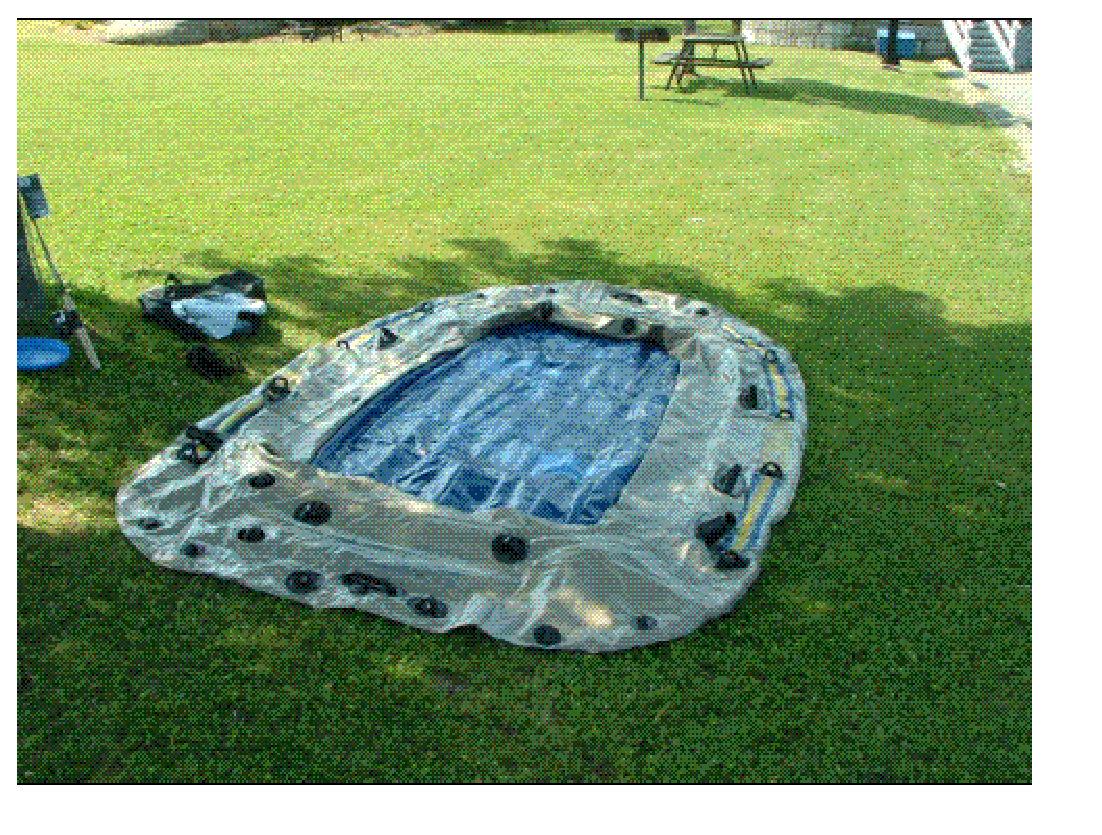
\epsfig{file=fig1.eps,width=3.5in}
Which one of the following is missing in it?
  
  
\noindent\hspace{3.0in} \begin{tabular}{|l|}
\hline
Your choice \\
\hline
 \\ 
 \\ 
\hline
\end{tabular}
  
  
 
 
\noindent{\textbf{\large{
A.}}}
An airplane
 
 
\noindent{\textbf{\large{
B.}}}
An air-boat
 
 
\noindent{\textbf{\large{
C.}}}
Lawn
 
 
\noindent{\textbf{\large{
D.}}}
A frisbee
 
 
\noindent{\textbf{\large{
E.}}}
A truck
 
 
\noindent{\textbf{\large{
F.}}}
  Not any of aboves.
 
 
 
\vspace{0.3in}
  
\vspace{0.2in}
  
         \begin{tabular}{|l|}
\hline
 Your marks  \\
\hline
 \\ 
 \\ 
\hline
\end{tabular}
\hspace{0.05in} \begin{tabular}{|l|}
\hline
 Full marks  \\
\hline
 \\ 
12.50 \\
\hline
\end{tabular}
{\textbf{\Large{Question
30.1.2 
}}}
  
  
In a hotel, the possiblity of  % 
smoking customer is
$a =  % 
0.730$, and the possiblity of  % 
equal-or-above 30 years old customer is $ b =  % 
0.7600$.
Please fill the following form.
 
\noindent
\begin{tabular}{|l|l|}
\hline
Customer & Possibility \\
\hline
smoking  and   % 
equal-or-above 30 years old  & \\
\hline
smoking  and   % 
under 30 years old & \\
\hline
 non-smoking and   % 
equal-or-above 30 years old  & \\
\hline
 non-smoking and  % 
under 30 years old & \\
\hline
\end{tabular}
 
 
 

 

 
\vspace{0.3in}
  
\vspace{0.2in}
  
         \begin{tabular}{|l|}
\hline
 Your marks  \\
\hline
 \\ 
 \\ 
\hline
\end{tabular}
\hspace{0.05in} \begin{tabular}{|l|}
\hline
 Full marks  \\
\hline
 \\ 
12.50 \\
\hline
\end{tabular}
{\textbf{\Large{Question
30.1.3 
}}}
  
  
 
An object is subjected to an external net force $\mathbf{f}=(
80.0,  % 
2.0,
-7000.0  )N$. Its mass is known as
$m= % 
58.0 kg$. Please calculate its accelaration.
 
 

 

 
\vspace{0.3in}
  
\vspace{0.2in}
  
         \begin{tabular}{|l|}
\hline
 Your marks  \\
\hline
 \\ 
 \\ 
\hline
\end{tabular}
\hspace{0.05in} \begin{tabular}{|l|}
\hline
 Full marks  \\
\hline
 \\ 
12.50 \\
\hline
\end{tabular}
{\textbf{\Large{Question
30.1.4 
}}}
  
  
Let us use Newton's Law of Universal Gravitation to calculate the force
of the Sun acting on the eight planets. Let us suppose the mass of the
Sun is $ % 
3.00 \times 10^{24} kg$. With the mass and the
distance to the Sun of each planet in the following table, please fill
the blanks for the forces.
 
\vspace{0.2in}
 
 
\begin{tabular}{|l|l|l|l|}
\hline
The Planet & Mass ($kg$) & Distanace from Sun ($m$) & The Force ($N$)\\
\hline
Mercury  &
           $ % 
3.00000000 \times 10^{24} $   &
             $ % 
7.000000000 \times 10^{24} $    &
\\  \hline
Venus    &
           $ % 
3.00 \times 10^{24} $    &
             $ % 
5.00 \times 10^{24} $    &
\\  \hline
Earth    &
           $ % 
9.00 \times 10^{24} $    &
             $ % 
8.00 \times 10^{24} $    &
\\   \hline
Mars     &
           $ % 
9.00 \times 10^{24} $    &
             $ % 
3.00 \times 10^{24} $    &
\\   \hline
Jupiter  &
           $ % 
7.00 \times 10^{24} $    &
             $ % 
5.00 \times 10^{24} $    &
\\  \hline
Saturn   &
           $ % 
1.000 \times 10^{25}$    &
             $ % 
8.00 \times 10^{24}$    &
\\  \hline
Uranus   &
           $ % 
6.00 \times 10^{24} $    &
             $ % 
9.00 \times 10^{24} $    &
\\  \hline
Neptune  &
           $ % 
6.00 \times 10^{24} $    &
             $ % 
7.00 \times 10^{24} $    &
\\  \hline
 
\end{tabular}
 
 

 
 

 
\vspace{0.3in}
  
\vspace{0.2in}
  
         \begin{tabular}{|l|}
\hline
 Your marks  \\
\hline
 \\ 
 \\ 
\hline
\end{tabular}
\hspace{0.05in} \begin{tabular}{|l|}
\hline
 Full marks  \\
\hline
 \\ 
12.50 \\
\hline
\end{tabular}
{\textbf{\Large{Question
30.1.5 
}}}
  
  
 
An object is subjected to an external net force $\mathbf{f}=(
60.0 ,
6.0,
-3000.0  )N$. Its mass is known as
$m= % 
56.0  kg$. Please choose the correct accelaration
from the following choices.
 
  
  
\noindent\hspace{3.0in} \begin{tabular}{|l|}
\hline
Your choice \\
\hline
 \\ 
 \\ 
\hline
\end{tabular}
  
  
 
 
\noindent{\textbf{\large{
A.}}}
The accelaration is
$(
2.9098ms^{-2},
0.10714ms^{-2},
1.9567 \times 10^{6}km/h^2
).
$
 
 
\noindent{\textbf{\large{
B.}}}
The accelaration is
$(
1.0714ms^{-2},
0.46937ms^{-2},
-694286.km/h^2
).
$
 
 
\noindent{\textbf{\large{
C.}}}
The accelaration is
$(
1.0714ms^{-2},
0.10714ms^{-2},
-694286.km/h^2
).
$
 
 
\noindent{\textbf{\large{
D.}}}
The accelaration is
$(
2.9098ms^{-2},
0.46937ms^{-2},
1.9567 \times 10^{6}km/h^2
).
$
 
 
\noindent{\textbf{\large{
E.}}}
none of these.
 
 
 
 

 
\vspace{0.3in}
  
\vspace{0.2in}
  
         \begin{tabular}{|l|}
\hline
 Your marks  \\
\hline
 \\ 
 \\ 
\hline
\end{tabular}
\hspace{0.05in} \begin{tabular}{|l|}
\hline
 Full marks  \\
\hline
 \\ 
12.50 \\
\hline
\end{tabular}
{\textbf{\Large{Question
30.1.6 
}}}
  
  
 
An object is subjected to an external net force $\mathbf{f}=(
30.0 ,
2.0,
-6000.0  )N$. Its mass is known as
$m= % 
54.0  kg$. Please choose the correct accelaration
from the following choices.
 
  
  
\noindent\hspace{3.0in} \begin{tabular}{|l|}
\hline
Your choice \\
\hline
 \\ 
 \\ 
\hline
\end{tabular}
  
  
 
 
\noindent{\textbf{\large{
A.}}}
The accelaration (vector) is
$(
7200.0,
480.00 ,
-4.7594 \times 10^{6}
)km/h^2.
$
 
 
\noindent{\textbf{\large{
B.}}}
The accelaration (vector) is
$(
7200.0,
480.00 ,
-1.4400 \times 10^{6}
)km/h^2.
$
 
 
\noindent{\textbf{\large{
C.}}}
The accelaration (vector) is
$(
27380.,
480.00 ,
3.7975 \times 10^{6}
)km/h^2.
$
 
 
\noindent{\textbf{\large{
D.}}}
The accelaration (vector) is
$(
-20827.,
480.00 ,
7.0625 \times 10^{6}
)km/h^2.
$
 
 
\noindent{\textbf{\large{
E.}}}
The accelaration (vector) is
$(
27380.,
480.00 ,
-4.7594 \times 10^{6}
)km/h^2.
$
 
 
\noindent{\textbf{\large{
F.}}}
The accelaration (vector) is
$(
-20827.,
480.00 ,
3.7975 \times 10^{6}
)km/h^2.
$
 
 
\noindent{\textbf{\large{
G.}}}
The accelaration (vector) is
$(
27380.,
480.00 ,
-1.4400 \times 10^{6}
)km/h^2.
$
 
 
\noindent{\textbf{\large{
H.}}}
The accelaration (vector) is
$(
31230.,
480.00 ,
-1.4400 \times 10^{6}
)km/h^2.
$
 
 
\noindent{\textbf{\large{
I.}}}
The accelaration (vector) is
$(
7200.0,
480.00 ,
7.0625 \times 10^{6}
)km/h^2.
$
 
 
\noindent{\textbf{\large{
J.}}}
The accelaration (vector) is
$(
27380.,
480.00 ,
7.0625 \times 10^{6}
)km/h^2.
$
 
 
\noindent{\textbf{\large{
K.}}}
The accelaration (vector) is
$(
31230.,
480.00 ,
3.7975 \times 10^{6}
)km/h^2.
$
 
 
\noindent{\textbf{\large{
L.}}}
The accelaration (vector) is
$(
7200.0,
480.00 ,
3.7975 \times 10^{6}
)km/h^2.
$
 
 
 
 

 
 
\vspace{0.3in}
   
   
\vspace{0.3in}
{\textbf{\LARGE{You have done all the above? A very good beginning, please go ahead.}}}
More constants the
Mass of electron
$m_e$$ =
9.109390 \times 10^{-31} $
kg
,
Universal gas constant
$R$$ =
8.315 $
J/(mol$\cdot $K)
,
$e$$ =
1.60217733 \times 10^{-19} $
C
, and
$m_p$$ =
1.6726231 \times 10^{-27} $
kg
%
may be very helpful.
\vspace{0.3in}
   
   
  
\vspace{0.2in}
  
\noindent\begin{tabular}{|l|}
\hline
 YOUR MARKS  \\
\hline
 \\ 
 \\ 
\hline
\end{tabular}
\hspace{0.05in} \begin{tabular}{|l|}
\hline
 Full Marks  \\
\hline
 \\ 
1.56 \\
\hline
\end{tabular}
{\textbf{\Large{QUESTION
30.2 
}}}
  
  
If any one of the following statements is correct, please fill the box ahead of it with $T$ .
If wrong, fill with $F$.
 
\noindent\begin{tabular}{|l|l|}\hline Your&\hspace{.2in} \\ answer&\hspace{.2in} \\ \hline \end{tabular}
1. $ % 
28$ is an  % 
even number.
 
\noindent\begin{tabular}{|l|l|}\hline Your&\hspace{.2in} \\ answer&\hspace{.2in} \\ \hline \end{tabular}
2.  % 
Montreal is in  % 
Ontario province.
 
\noindent\begin{tabular}{|l|l|}\hline Your&\hspace{.2in} \\ answer&\hspace{.2in} \\ \hline \end{tabular}
3.  % 
$\mathbf{F}=m\mathbf{a}$ is a mathmatical form of
the Newton's Second Law.
 

 
\vspace{0.3in}
  
\vspace{0.2in}
  
\noindent\begin{tabular}{|l|}
\hline
 YOUR MARKS  \\
\hline
 \\ 
 \\ 
\hline
\end{tabular}
\hspace{0.05in} \begin{tabular}{|l|}
\hline
 Full Marks  \\
\hline
 \\ 
1.56 \\
\hline
\end{tabular}
{\textbf{\Large{QUESTION
30.3 
}}}
  
  
Please choose the correct one from the following statements:
  
  
\noindent\hspace{3.0in} \begin{tabular}{|l|}
\hline
Your choice \\
\hline
 \\ 
 \\ 
\hline
\end{tabular}
  
  
 
 
\noindent{\textbf{\large{
A.}}}
Canada has  %
33 provinces and  %
38 territories.
 
 
\noindent{\textbf{\large{
B.}}}
Canada has  %
35 provinces and  %
34 territories.
 
 
\noindent{\textbf{\large{
C.}}}
Canada has  %
37 provinces and  %
37 territories.
 
 
\noindent{\textbf{\large{
D.}}}
Canada has  %
36 provinces and  %
35 territories.
 
 
\noindent{\textbf{\large{
E.}}}
Canada has  %
34 provinces and  %
39 territories.
 
 
\noindent{\textbf{\large{
F.}}}
 None of above.
 
 
  
\vspace{0.2in}
  
\noindent\begin{tabular}{|l|}
\hline
 YOUR MARKS  \\
\hline
 \\ 
 \\ 
\hline
\end{tabular}
\hspace{0.05in} \begin{tabular}{|l|}
\hline
 Full Marks  \\
\hline
 \\ 
3.12 \\
\hline
\end{tabular}
{\textbf{\Large{QUESTION
30.4 
}}}
  
  
 
 
An object is subjected to an external net force $\mathbf{f}=
(20.0 , 4.0 , -6000.0) N$.
Its mass is known as $m= % 
52.0000 kg$. Please choose the
correct accelaration from the following choices.
 
  
  
\noindent\hspace{3.0in} \begin{tabular}{|l|}
\hline
Your choice \\
\hline
 \\ 
 \\ 
\hline
\end{tabular}
  
  
 
 
\noindent{\textbf{\large{
A.}}}
The accelaration is $  %
(
0.385,
7.7 \times 10^{-2},
526.04)
ms^{-2} $.
 
 
\noindent{\textbf{\large{
B.}}}
The accelaration is $  %
(
0.385,
7.7 \times 10^{-2},
-115.38)
ms^{-2} $.
 
 
\noindent{\textbf{\large{
C.}}}
The accelaration is $  %
(
0.385,
0.23,
-115.38)
ms^{-2} $.
 
 
\noindent{\textbf{\large{
D.}}}
The accelaration is $  %
(
4.34,
7.7 \times 10^{-2},
-115.38)
ms^{-2} $.
 
 
\noindent{\textbf{\large{
E.}}}
The accelaration is $  %
(
4.34,
0.23,
526.04)
ms^{-2} $.
 
 
\noindent{\textbf{\large{
F.}}}
The accelaration is $  %
(
0.385,
0.23,
526.04)
ms^{-2} $.
 
 
\noindent{\textbf{\large{
G.}}}
The accelaration is $  %
(
4.34,
7.7 \times 10^{-2},
526.04)
ms^{-2} $.
 
 
\noindent{\textbf{\large{
H.}}}
The accelaration is $  %
(
4.34,
0.23,
-115.38)
ms^{-2} $.
 
 
 

 

 
\vspace{0.3in}
  
\vspace{0.2in}
  
\noindent\begin{tabular}{|l|}
\hline
 YOUR MARKS  \\
\hline
 \\ 
 \\ 
\hline
\end{tabular}
\hspace{0.05in} \begin{tabular}{|l|}
\hline
 Full Marks  \\
\hline
 \\ 
3.12 \\
\hline
\end{tabular}
{\textbf{\Large{QUESTION
30.5 
}}}
  
  
Considering case-insensitivity, please match the following same strings.
  
  
\begin{tabular}{|l|l|l|}
 \hline
 Column Left & Column Right  & Your choinces \\ 
 \hline
{\textbf{\large{
A.}}}
A
  & 
b
 & 
 \\ 
 \hline
{\textbf{\large{
B.}}}
 A= %
6/ %
2

  & 
ER
 & 
 \\ 
 \hline
{\textbf{\large{
C.}}}
Er
  & 
eR
 & 
 \\ 
 \hline
{\textbf{\large{
D.}}}
B
  & 
 a= %
3
 & 
 \\ 
 \hline
{\textbf{\large{
E.}}}
er
  & 
a
 & 
 \\ 
 \hline
 \end{tabular}
  
  
 
  
\vspace{0.2in}
  
\noindent\begin{tabular}{|l|}
\hline
 YOUR MARKS  \\
\hline
 \\ 
 \\ 
\hline
\end{tabular}
\hspace{0.05in} \begin{tabular}{|l|}
\hline
 Full Marks  \\
\hline
 \\ 
1.56 \\
\hline
\end{tabular}
{\textbf{\Large{QUESTION
30.6 
}}}
  
  
 
An object is subjected to an external net force $\mathbf{f}=(
20.000 ,
3.0000,
-2000.0  )N$. Its mass is known as
$m= % 
60.0000  kg$. Please choose the correct accelaration
from the following choices.
 
  
  
\noindent\hspace{3.0in} \begin{tabular}{|l|}
\hline
Your choice \\
\hline
 \\ 
 \\ 
\hline
\end{tabular}
  
  
 
 
\noindent{\textbf{\large{
A.}}}
The accelaration is
$(
0.33333ms^{-2},
648.00km/h^2,
116.36ms^{-2}
).
$
 
 
\noindent{\textbf{\large{
B.}}}
The accelaration is
$(
0.33333ms^{-2},
648.00km/h^2,
-33.333ms^{-2}
).
$
 
 
\noindent{\textbf{\large{
C.}}}
The accelaration is
$(
0.33333ms^{-2},
1945.9km/h^2,
-33.333ms^{-2}
).
$
 
 
\noindent{\textbf{\large{
D.}}}
The accelaration is
$(
-0.96447ms^{-2},
1945.9km/h^2,
-33.333ms^{-2}
).
$
 
 
\noindent{\textbf{\large{
E.}}}
The accelaration is
$(
-0.96447ms^{-2},
648.00km/h^2,
-33.333ms^{-2}
).
$
 
 
\noindent{\textbf{\large{
F.}}}
The accelaration is
$(
0.33333ms^{-2},
1945.9km/h^2,
116.36ms^{-2}
).
$
 
 
\noindent{\textbf{\large{
G.}}}
 None of these.
 
 
 
 

 
\vspace{0.3in}
   
   
\vspace{0.3in}
{\textbf{\LARGE{You have done all the above? Excellent! Not much left, please continue.}}}
\vspace{0.3in}
   
   
  
\vspace{0.2in}
  
\noindent\begin{tabular}{|l|}
\hline
 YOUR MARKS  \\
\hline
 \\ 
 \\ 
\hline
\end{tabular}
\hspace{0.05in} \begin{tabular}{|l|}
\hline
 Full Marks  \\
\hline
 \\ 
12.50 \\
\hline
\end{tabular}
{\textbf{\Large{QUESTION
30.7 
}}}
  
  
 
An object is subjected to an external net force $\mathbf{f}=
(60.0 , 3.0 , -6000.0) N$.
Its mass is known as $m= % 
54.0 kg$.
Please choose the correct accelaration from the following choices.
  
  
\noindent\hspace{3.0in} \begin{tabular}{|l|}
\hline
Your choice \\
\hline
 \\ 
 \\ 
\hline
\end{tabular}
  
  
 
 
\noindent{\textbf{\large{
A.}}}
  The accelaration is $  %
(
1.11,
5.6 \times 10^{-2},
-111.11)
ms^{-2} $.
 
 
\noindent{\textbf{\large{
B.}}}
  The accelaration is $  %
(
3.83,
5.6 \times 10^{-2},
-111.11)
ms^{-2} $.
 
 
\noindent{\textbf{\large{
C.}}}
  The accelaration is $  %
(
1.11,
5.6 \times 10^{-2},
356.81)
ms^{-2} $.
 
 
\noindent{\textbf{\large{
D.}}}
  The accelaration is $  %
(
3.83,
0.19,
356.81)
ms^{-2} $.
 
 
 

 
 
\vspace{0.3in}
  
\vspace{0.2in}
  
\noindent\begin{tabular}{|l|}
\hline
 YOUR MARKS  \\
\hline
 \\ 
 \\ 
\hline
\end{tabular}
\hspace{0.05in} \begin{tabular}{|l|}
\hline
 Full Marks  \\
\hline
 \\ 
12.50 \\
\hline
\end{tabular}
{\textbf{\Large{QUESTION
30.8 
}}}
  
  
 
$ \left( \begin{array}{ccccccccc}
           4  & 
           6  & 
           7  & 
           5  \\ 
           5  & 
           4  & 
           5  & 
           6  \\ 
           5  & 
           4  & 
           5  & 
           6
\end{array}\right) \times
\left( \begin{array}{c}
           2  \\ 
           2  \\ 
           2  \\ 
           2
\end{array}\right) $ =?
 
 
$  % 
 \left( \begin{array}
 {
 c
 c
 }
 \Lambda & 
 \Psi \\ 
 \sigma & 
 \Upsilon \\ 
 \beta & 
 \beta \\ 
 \Phi & 
 \Theta
 \end{array} \right)
 \left( \begin{array}
 {
 c
 }
 \beta \\ 
 \beta
 \end{array} \right)
$ =?
 

 

 
\vspace{0.3in}
  
\vspace{0.2in}
  
\noindent\begin{tabular}{|l|}
\hline
 YOUR MARKS  \\
\hline
 \\ 
 \\ 
\hline
\end{tabular}
\hspace{0.05in} \begin{tabular}{|l|}
\hline
 Full Marks  \\
\hline
 \\ 
1.56 \\
\hline
\end{tabular}
{\textbf{\Large{QUESTION
30.9 
}}}
  
  
 
 
% First root
% Second root

 
Please solve the following equation:
\begin{eqnarray*}
-9 \times x^2  % 
+  % 
63
                 \times x    % 
+  % 
1530 =0
\end{eqnarray*}
 

 

 
\vspace{0.3in}
   
   
 \vspace{0.2in}
Here are still some constants for use:
 
 
\noindent\begin{tabular}{|l|l|l|}
\hline
Constant & Symbol & Value \\
\hline
 
Mass of proton &
$m_p$ &
 $ 1.6726231 \times 10^{-27} $
kg \\
\hline
 
Boltzmann's constant &
$k$ &
 $ 1.381 \times 10^{-23} $
J/K \\
\hline
 
\end{tabular}
 
Thank you very much for answering these questions!
 
{\textbf{\large{Please be advised}}} that in this paper there are questions from
30.1 through
30.9.
And any one of them may contain more than one sub-question, thus the total number
of sub-questions here is around 14, of which
13 should be answered.
 
   
   
   
   
\vspace{1.0in} 
{\textbf{\large{ *** END OF PAPER, THANKS *** }}} 
   
   
\hspace{1.0in} By: 
         239 (          26 ,           34 )
   
   
   
   
\newpage 
\setcounter{page}{ 
    31001 } 
   
   
   
   
\noindent\begin{tabular}{|l|}
\hline
YOUR NAME (FIRST, ... LAST)  \\
\hline
 \\ 
 \\ 
\hline
\end{tabular}
\hspace{0.05in} \begin{tabular}{|l|}
\hline
 YOUR   ID   INFORMATION  \\
\hline
 \\ 
 \\ 
\hline
\end{tabular}
   
   
\vspace{0.2in}\noindent\begin{tabular}{|l|}
\hline
YOUR TOTAL MARKS  \\
\hline
 \\ 
 \\ 
\hline
\end{tabular}
\hspace{0.05in} \begin{tabular}{|l|}
\hline
TOTAL FULL MARKS  \\
\hline
 \\ 
100.00 \\
\hline
\end{tabular}
   
   
 \vspace{0.2in}
 
 
{\Huge  THIS IS AN EXAMPLE OF}
 
{\Huge  PERSONALIZED TESTS. }
 
If needed, please use the following constants.
 
 
 
\noindent\begin{tabular}{|l|l|l|}
\hline
Constant & Symbol & Value \\
\hline
Acceleration due to earth's gravity &
$g$ &
 $ 9.80 $
m/s$^2$ \\
\hline
Avogadro's number &
$N_A$ &
 $ 6.0221367 \times 10^{23} $
mol$^{-1}$ \\
\hline
Boltzmann's constant &
$k$ &
 $ 1.380658 \times 10^{-23} $
J/K \\
\hline
Coulomb's constant &
$k$ &
 $ 8.99 \times 10^{9} $
N$\cdot $m$^2$/C$^2$ \\
\hline
Electron charge magnitiude &
$e$ &
 $ 1.60217733 \times 10^{-19} $
C \\
\hline
Permeability of free space &
$\mu _0$ &
 $ 1.25663706 \times 10^{-6} $
T$\cdot $m/A \\
\hline
Permittivity of free space &
$\epsilon _0$ &
 $ 8.854187817 \times 10^{-12} $
C$^2$/(N$\cdot $m$^2$) \\
\hline
Pi &
$\pi$ &
 $ 3.14159265 $
$ $ \\
\hline
Planck's constant &
$h$ &
 $ 6.6260755 \times 10^{-34} $
J$\cdot $s \\
\hline
Mass of electron &
$m_e$ &
 $ 9.1093897 \times 10^{-31} $
kg \\
\hline
\end{tabular}
 
 
\noindent\begin{tabular}{|l|l|l|}
\hline
Constant & Symbol & Value \\
\hline
Mass of neutron &
$m_n$ &
 $ 1.6749286 \times 10^{-27} $
kg \\
\hline
Mass of proton &
$m_p$ &
 $ 1.6726231 \times 10^{-27} $
kg \\
\hline
Speed of light in vacuum &
$c$ &
 $ 299792458. $
m/s \\
\hline
Universal gravitational constant &
$G$ &
 $ 6.67259 \times 10^{-11} $
N$\cdot $m$^2$/kg$^2$ \\
\hline
Universal gas constant &
$R$ &
 $ 8.314510 $
J/(mol$\cdot $K) \\
\hline
\end{tabular}
 
 
{\textbf{\large{Please be advised}}} that in this paper there are questions from
31.1 through
31.9.
And any one of them may contain more than one sub-question, thus the total number
of sub-questions here is around 14, of which
13 should be answered.
 
\vspace{0.3in}
 
 
   
   
  
\vspace{0.2in}
  
\noindent\begin{tabular}{|l|}
\hline
 YOUR MARKS  \\
\hline
 \\ 
 \\ 
\hline
\end{tabular}
\hspace{0.05in} \begin{tabular}{|l|}
\hline
 Full Marks  \\
\hline
 \\ 
62.50 \\
\hline
\end{tabular}
{\textbf{\Large{QUESTION
31.1 
}}}
  
  
 
{\textbf{\Large{Please answer ONLY
5 of the following
6 questions (Questions
31.1.1 through
31.1.6). }}}
 
Here are still some constants for use in the following questions:
 
 
\noindent\begin{tabular}{|l|l|l|}
\hline
Constant & Symbol & Value \\
\hline
 
Boltzmann's constant &
$k$ &
 $ 1.381 \times 10^{-23} $
J/K \\
\hline
 
Avogadro's number &
$N_A$ &
 $ 6.022 \times 10^{23} $
mol$^{-1}$ \\
\hline
 
Mass of electron &
$m_e$ &
 $ 9.1093897 \times 10^{-31} $
kg \\
\hline
 
\end{tabular}
 
  
\vspace{0.2in}
  
         \begin{tabular}{|l|}
\hline
 Your marks  \\
\hline
 \\ 
 \\ 
\hline
\end{tabular}
\hspace{0.05in} \begin{tabular}{|l|}
\hline
 Full marks  \\
\hline
 \\ 
12.50 \\
\hline
\end{tabular}
{\textbf{\Large{Question
31.1.1 
}}}
  
  
In a hotel, the possiblity of  % 
smoking customer is
$a =  % 
0.240$, and the possiblity of  % 
equal or above 30 years old customer is $ b =  % 
2.00 \times 10^{-2}$.
Please calculate the possiblity of  % 
 non-smoking and  % 
under 30 years old customer.
 

 

 
\vspace{0.3in}
  
\vspace{0.2in}
  
         \begin{tabular}{|l|}
\hline
 Your marks  \\
\hline
 \\ 
 \\ 
\hline
\end{tabular}
\hspace{0.05in} \begin{tabular}{|l|}
\hline
 Full marks  \\
\hline
 \\ 
12.50 \\
\hline
\end{tabular}
{\textbf{\Large{Question
31.1.2 
}}}
  
  
 
An object is subjected to an external net force $\mathbf{f}=(
20.0 ,
2.0,
-4000.0  )N$. Its mass is known as
$m= % 
54.0  kg$. Please choose the correct accelaration
from the following choices.
 
  
  
\noindent\hspace{3.0in} \begin{tabular}{|l|}
\hline
Your choice \\
\hline
 \\ 
 \\ 
\hline
\end{tabular}
  
  
 
 
\noindent{\textbf{\large{
A.}}}
The accelaration (vector) is
$(
-15958.,
480.00 ,
-960000.
)km/h^2.
$
 
 
\noindent{\textbf{\large{
B.}}}
The accelaration (vector) is
$(
18692.,
480.00 ,
-960000.
)km/h^2.
$
 
 
\noindent{\textbf{\large{
C.}}}
The accelaration (vector) is
$(
18692.,
480.00 ,
2.0503 \times 10^{6}
)km/h^2.
$
 
 
\noindent{\textbf{\large{
D.}}}
The accelaration (vector) is
$(
-15958.,
480.00 ,
3.2965 \times 10^{6}
)km/h^2.
$
 
 
\noindent{\textbf{\large{
E.}}}
The accelaration (vector) is
$(
18692.,
480.00 ,
-3.9936 \times 10^{6}
)km/h^2.
$
 
 
\noindent{\textbf{\large{
F.}}}
The accelaration (vector) is
$(
-15958.,
480.00 ,
-3.9936 \times 10^{6}
)km/h^2.
$
 
 
\noindent{\textbf{\large{
G.}}}
The accelaration (vector) is
$(
-15958.,
480.00 ,
2.0503 \times 10^{6}
)km/h^2.
$
 
 
\noindent{\textbf{\large{
H.}}}
The accelaration (vector) is
$(
18692.,
480.00 ,
3.2965 \times 10^{6}
)km/h^2.
$
 
 
\noindent{\textbf{\large{
I.}}}
The accelaration (vector) is
$(
-16677.,
480.00 ,
2.0503 \times 10^{6}
)km/h^2.
$
 
 
\noindent{\textbf{\large{
J.}}}
The accelaration (vector) is
$(
4800.0,
480.00 ,
-960000.
)km/h^2.
$
 
 
\noindent{\textbf{\large{
K.}}}
The accelaration (vector) is
$(
4800.0,
480.00 ,
3.2965 \times 10^{6}
)km/h^2.
$
 
 
\noindent{\textbf{\large{
L.}}}
The accelaration (vector) is
$(
-16677.,
480.00 ,
-960000.
)km/h^2.
$
 
 
 
 

 
 
\vspace{0.3in}
  
\vspace{0.2in}
  
         \begin{tabular}{|l|}
\hline
 Your marks  \\
\hline
 \\ 
 \\ 
\hline
\end{tabular}
\hspace{0.05in} \begin{tabular}{|l|}
\hline
 Full marks  \\
\hline
 \\ 
12.50 \\
\hline
\end{tabular}
{\textbf{\Large{Question
31.1.3 
}}}
  
  
In a hotel, the possiblity of  % 
non-smoking customer is
$a =  % 
0.910$, and the possiblity of  % 
equal-or-above 30 years old customer is $ b =  % 
0.5000$.
Please fill the following form.
 
\noindent
\begin{tabular}{|l|l|}
\hline
Customer & Possibility \\
\hline
smoking  and   % 
equal-or-above 30 years old  & \\
\hline
smoking  and   % 
under 30 years old & \\
\hline
 non-smoking and   % 
equal-or-above 30 years old  & \\
\hline
 non-smoking and  % 
under 30 years old & \\
\hline
\end{tabular}
 
 
 

 

 
\vspace{0.3in}
  
\vspace{0.2in}
  
         \begin{tabular}{|l|}
\hline
 Your marks  \\
\hline
 \\ 
 \\ 
\hline
\end{tabular}
\hspace{0.05in} \begin{tabular}{|l|}
\hline
 Full marks  \\
\hline
 \\ 
12.50 \\
\hline
\end{tabular}
{\textbf{\Large{Question
31.1.4 
}}}
  
  
 
An object is subjected to an external net force $\mathbf{f}=(
30.0 ,
2.0,
-2000.0  )N$. Its mass is known as
$m= % 
52.0  kg$. Please choose the correct accelaration
from the following choices.
 
  
  
\noindent\hspace{3.0in} \begin{tabular}{|l|}
\hline
Your choice \\
\hline
 \\ 
 \\ 
\hline
\end{tabular}
  
  
 
 
\noindent{\textbf{\large{
A.}}}
The accelaration is
$(
2.4439ms^{-2},
-0.18750ms^{-2},
-1.6744 \times 10^{6}km/h^2
).
$
 
 
\noindent{\textbf{\large{
B.}}}
The accelaration is
$(
2.4439ms^{-2},
3.8462 \times 10^{-2}ms^{-2},
-1.6744 \times 10^{6}km/h^2
).
$
 
 
\noindent{\textbf{\large{
C.}}}
The accelaration is
$(
0.57692ms^{-2},
-0.18750ms^{-2},
-1.6744 \times 10^{6}km/h^2
).
$
 
 
\noindent{\textbf{\large{
D.}}}
The accelaration is
$(
0.57692ms^{-2},
-0.18750ms^{-2},
-498462.km/h^2
).
$
 
 
\noindent{\textbf{\large{
E.}}}
none of these.
 
 
 
 

 
\vspace{0.3in}
  
\vspace{0.2in}
  
         \begin{tabular}{|l|}
\hline
 Your marks  \\
\hline
 \\ 
 \\ 
\hline
\end{tabular}
\hspace{0.05in} \begin{tabular}{|l|}
\hline
 Full marks  \\
\hline
 \\ 
12.50 \\
\hline
\end{tabular}
{\textbf{\Large{Question
31.1.5 
}}}
  
  
See the following picture.
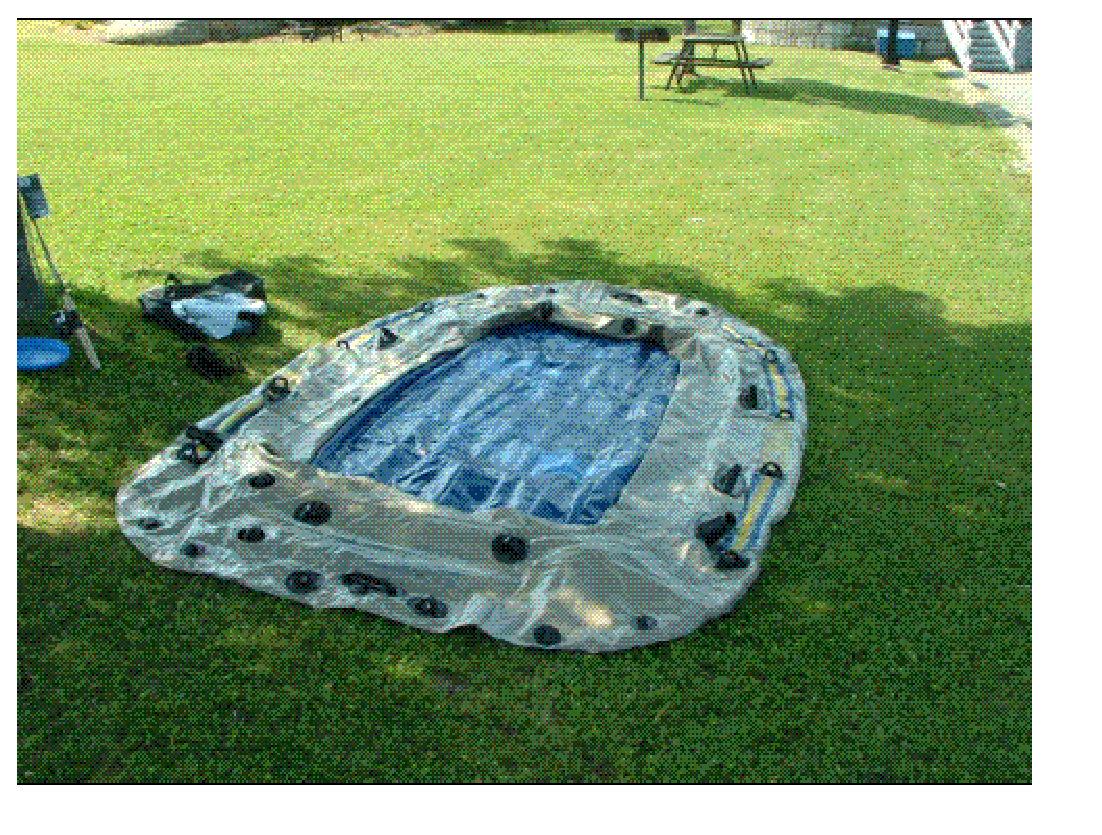
\epsfig{file=fig1.eps,width=3.5in}
Which one of the following is missing in it?
  
  
\noindent\hspace{3.0in} \begin{tabular}{|l|}
\hline
Your choice \\
\hline
 \\ 
 \\ 
\hline
\end{tabular}
  
  
 
 
\noindent{\textbf{\large{
A.}}}
An airplane
 
 
\noindent{\textbf{\large{
B.}}}
An air-boat
 
 
\noindent{\textbf{\large{
C.}}}
Lawn
 
 
\noindent{\textbf{\large{
D.}}}
A table
 
 
\noindent{\textbf{\large{
E.}}}
A frisbee
 
 
\noindent{\textbf{\large{
F.}}}
  Not any of aboves.
 
 
 
\vspace{0.3in}
  
\vspace{0.2in}
  
         \begin{tabular}{|l|}
\hline
 Your marks  \\
\hline
 \\ 
 \\ 
\hline
\end{tabular}
\hspace{0.05in} \begin{tabular}{|l|}
\hline
 Full marks  \\
\hline
 \\ 
12.50 \\
\hline
\end{tabular}
{\textbf{\Large{Question
31.1.6 
}}}
  
  
 
An object is subjected to an external net force $\mathbf{f}=(
60.0,  % 
5.0,
-6000.0  )N$. Its mass is known as
$m= % 
56.0 kg$. Please calculate its accelaration.
 
 

 

 
\vspace{0.3in}
   
   
\vspace{0.3in}
{\textbf{\LARGE{You have done all the above? A very good beginning, please go ahead.}}}
More constants the
Mass of electron
$m_e$$ =
9.109390 \times 10^{-31} $
kg
,
Universal gas constant
$R$$ =
8.315 $
J/(mol$\cdot $K)
,
$e$$ =
1.60217733 \times 10^{-19} $
C
, and
$m_p$$ =
1.6726231 \times 10^{-27} $
kg
%
may be very helpful.
\vspace{0.3in}
   
   
  
\vspace{0.2in}
  
\noindent\begin{tabular}{|l|}
\hline
 YOUR MARKS  \\
\hline
 \\ 
 \\ 
\hline
\end{tabular}
\hspace{0.05in} \begin{tabular}{|l|}
\hline
 Full Marks  \\
\hline
 \\ 
1.56 \\
\hline
\end{tabular}
{\textbf{\Large{QUESTION
31.2 
}}}
  
  
Please choose the correct one from the following statements:
  
  
\noindent\hspace{3.0in} \begin{tabular}{|l|}
\hline
Your choice \\
\hline
 \\ 
 \\ 
\hline
\end{tabular}
  
  
 
 
\noindent{\textbf{\large{
A.}}}
Canada has  %
35 provinces and  %
34 territories.
 
 
\noindent{\textbf{\large{
B.}}}
Canada has  %
37 provinces and  %
37 territories.
 
 
\noindent{\textbf{\large{
C.}}}
Canada has  %
34 provinces and  %
39 territories.
 
 
\noindent{\textbf{\large{
D.}}}
Canada has  %
33 provinces and  %
38 territories.
 
 
\noindent{\textbf{\large{
E.}}}
Canada has  %
36 provinces and  %
35 territories.
 
 
\noindent{\textbf{\large{
F.}}}
 None of above.
 
 
  
\vspace{0.2in}
  
\noindent\begin{tabular}{|l|}
\hline
 YOUR MARKS  \\
\hline
 \\ 
 \\ 
\hline
\end{tabular}
\hspace{0.05in} \begin{tabular}{|l|}
\hline
 Full Marks  \\
\hline
 \\ 
1.56 \\
\hline
\end{tabular}
{\textbf{\Large{QUESTION
31.3 
}}}
  
  
 
An object is subjected to an external net force $\mathbf{f}=(
80.000 ,
9.0000,
-5000.0  )N$. Its mass is known as
$m= % 
52.0000  kg$. Please choose the correct accelaration
from the following choices.
 
  
  
\noindent\hspace{3.0in} \begin{tabular}{|l|}
\hline
Your choice \\
\hline
 \\ 
 \\ 
\hline
\end{tabular}
  
  
 
 
\noindent{\textbf{\large{
A.}}}
The accelaration is
$(
5.1859ms^{-2},
2243.1km/h^2,
-96.154ms^{-2}
).
$
 
 
\noindent{\textbf{\large{
B.}}}
The accelaration is
$(
5.1859ms^{-2},
4767.8km/h^2,
441.36ms^{-2}
).
$
 
 
\noindent{\textbf{\large{
C.}}}
The accelaration is
$(
1.5385ms^{-2},
2243.1km/h^2,
-96.154ms^{-2}
).
$
 
 
\noindent{\textbf{\large{
D.}}}
The accelaration is
$(
5.1859ms^{-2},
2243.1km/h^2,
441.36ms^{-2}
).
$
 
 
\noindent{\textbf{\large{
E.}}}
The accelaration is
$(
1.5385ms^{-2},
4767.8km/h^2,
-96.154ms^{-2}
).
$
 
 
\noindent{\textbf{\large{
F.}}}
The accelaration is
$(
1.5385ms^{-2},
2243.1km/h^2,
441.36ms^{-2}
).
$
 
 
\noindent{\textbf{\large{
G.}}}
 None of these.
 
 
 
 

 
\vspace{0.3in}
  
\vspace{0.2in}
  
\noindent\begin{tabular}{|l|}
\hline
 YOUR MARKS  \\
\hline
 \\ 
 \\ 
\hline
\end{tabular}
\hspace{0.05in} \begin{tabular}{|l|}
\hline
 Full Marks  \\
\hline
 \\ 
3.12 \\
\hline
\end{tabular}
{\textbf{\Large{QUESTION
31.4 
}}}
  
  
Considering case-insensitivity, please match the following same strings.
  
  
\begin{tabular}{|l|l|l|}
 \hline
 Column Left & Column Right  & Your choinces \\ 
 \hline
{\textbf{\large{
A.}}}
B
  & 
YJH
 & 
 \\ 
 \hline
{\textbf{\large{
B.}}}
asdf(:)
  & 
 a= %
4
 & 
 \\ 
 \hline
{\textbf{\large{
C.}}}
 A= %
8/ %
2

  & 
c
 & 
 \\ 
 \hline
{\textbf{\large{
D.}}}
C
  & 
b
 & 
 \\ 
 \hline
{\textbf{\large{
E.}}}
yjh
  & 
ASDF(:)
 & 
 \\ 
 \hline
 \end{tabular}
  
  
 
  
\vspace{0.2in}
  
\noindent\begin{tabular}{|l|}
\hline
 YOUR MARKS  \\
\hline
 \\ 
 \\ 
\hline
\end{tabular}
\hspace{0.05in} \begin{tabular}{|l|}
\hline
 Full Marks  \\
\hline
 \\ 
1.56 \\
\hline
\end{tabular}
{\textbf{\Large{QUESTION
31.5 
}}}
  
  
If any one of the following statements is correct, please fill the box ahead of it with $T$ .
If wrong, fill with $F$.
 
\noindent\begin{tabular}{|l|l|}\hline Your&\hspace{.2in} \\ answer&\hspace{.2in} \\ \hline \end{tabular}
1. $ % 
50$ is an  % 
even number.
 
\noindent\begin{tabular}{|l|l|}\hline Your&\hspace{.2in} \\ answer&\hspace{.2in} \\ \hline \end{tabular}
2.  % 
Montreal is in  % 
Ontario province.
 
\noindent\begin{tabular}{|l|l|}\hline Your&\hspace{.2in} \\ answer&\hspace{.2in} \\ \hline \end{tabular}
3.  % 
$\mathbf{F}=m\mathbf{a}$ is a mathmatical form of
the Newton's Second Law.
 

 
\vspace{0.3in}
  
\vspace{0.2in}
  
\noindent\begin{tabular}{|l|}
\hline
 YOUR MARKS  \\
\hline
 \\ 
 \\ 
\hline
\end{tabular}
\hspace{0.05in} \begin{tabular}{|l|}
\hline
 Full Marks  \\
\hline
 \\ 
3.12 \\
\hline
\end{tabular}
{\textbf{\Large{QUESTION
31.6 
}}}
  
  
 
 
An object is subjected to an external net force $\mathbf{f}=
(40.0 , 3.0 , -6000.0) N$.
Its mass is known as $m= % 
52.0000 kg$. Please choose the
correct accelaration from the following choices.
 
  
  
\noindent\hspace{3.0in} \begin{tabular}{|l|}
\hline
Your choice \\
\hline
 \\ 
 \\ 
\hline
\end{tabular}
  
  
 
 
\noindent{\textbf{\large{
A.}}}
The accelaration is $  %
(
-1.89,
0.26,
-115.38)
ms^{-2} $.
 
 
\noindent{\textbf{\large{
B.}}}
The accelaration is $  %
(
0.769,
5.8 \times 10^{-2},
-115.38)
ms^{-2} $.
 
 
\noindent{\textbf{\large{
C.}}}
The accelaration is $  %
(
-1.89,
5.8 \times 10^{-2},
-115.38)
ms^{-2} $.
 
 
\noindent{\textbf{\large{
D.}}}
The accelaration is $  %
(
-1.89,
0.26,
-412.14)
ms^{-2} $.
 
 
\noindent{\textbf{\large{
E.}}}
The accelaration is $  %
(
0.769,
0.26,
-115.38)
ms^{-2} $.
 
 
\noindent{\textbf{\large{
F.}}}
The accelaration is $  %
(
0.769,
0.26,
-412.14)
ms^{-2} $.
 
 
\noindent{\textbf{\large{
G.}}}
The accelaration is $  %
(
0.769,
5.8 \times 10^{-2},
-412.14)
ms^{-2} $.
 
 
\noindent{\textbf{\large{
H.}}}
The accelaration is $  %
(
-1.89,
5.8 \times 10^{-2},
-412.14)
ms^{-2} $.
 
 
 

 

 
\vspace{0.3in}
   
   
\vspace{0.3in}
{\textbf{\LARGE{You have done all the above? Excellent! Not much left, please continue.}}}
\vspace{0.3in}
   
   
  
\vspace{0.2in}
  
\noindent\begin{tabular}{|l|}
\hline
 YOUR MARKS  \\
\hline
 \\ 
 \\ 
\hline
\end{tabular}
\hspace{0.05in} \begin{tabular}{|l|}
\hline
 Full Marks  \\
\hline
 \\ 
12.50 \\
\hline
\end{tabular}
{\textbf{\Large{QUESTION
31.7 
}}}
  
  
 
$ \left( \begin{array}{ccccccccc}
           5  & 
           6  & 
           6  & 
           6  \\ 
           6  & 
           4  & 
           4  & 
           4  \\ 
           5  & 
           6  & 
           5  & 
           5
\end{array}\right) \times
\left( \begin{array}{c}
           2  \\ 
           2  \\ 
           2  \\ 
           2
\end{array}\right) $ =?
 
 
$  % 
 \left( \begin{array}
 {
 c
 c
 }
 \Theta & 
 \delta \\ 
                    \Xi & 
 \varepsilon \\ 
 \delta & 
 \beta \\ 
 \Phi & 
                    \Xi
 \end{array} \right)
 \left( \begin{array}
 {
 c
 }
 \gamma \\ 
 \beta
 \end{array} \right)
$ =?
 

 

 
\vspace{0.3in}
  
\vspace{0.2in}
  
\noindent\begin{tabular}{|l|}
\hline
 YOUR MARKS  \\
\hline
 \\ 
 \\ 
\hline
\end{tabular}
\hspace{0.05in} \begin{tabular}{|l|}
\hline
 Full Marks  \\
\hline
 \\ 
12.50 \\
\hline
\end{tabular}
{\textbf{\Large{QUESTION
31.8 
}}}
  
  
 
An object is subjected to an external net force $\mathbf{f}=
(90.0 , 5.0 , -3000.0) N$.
Its mass is known as $m= % 
52.0 kg$.
Please choose the correct accelaration from the following choices.
  
  
\noindent\hspace{3.0in} \begin{tabular}{|l|}
\hline
Your choice \\
\hline
 \\ 
 \\ 
\hline
\end{tabular}
  
  
 
 
\noindent{\textbf{\large{
A.}}}
  The accelaration is $  %
(
1.73,
9.6 \times 10^{-2},
254.30)
ms^{-2} $.
 
 
\noindent{\textbf{\large{
B.}}}
  The accelaration is $  %
(
-5.03,
9.6 \times 10^{-2},
254.30)
ms^{-2} $.
 
 
\noindent{\textbf{\large{
C.}}}
  The accelaration is $  %
(
1.73,
9.6 \times 10^{-2},
-57.692)
ms^{-2} $.
 
 
\noindent{\textbf{\large{
D.}}}
  The accelaration is $  %
(
1.73,
0.33,
254.30)
ms^{-2} $.
 
 
 

 
 
\vspace{0.3in}
  
\vspace{0.2in}
  
\noindent\begin{tabular}{|l|}
\hline
 YOUR MARKS  \\
\hline
 \\ 
 \\ 
\hline
\end{tabular}
\hspace{0.05in} \begin{tabular}{|l|}
\hline
 Full Marks  \\
\hline
 \\ 
1.56 \\
\hline
\end{tabular}
{\textbf{\Large{QUESTION
31.9 
}}}
  
  
 
 
% First root
% Second root

 
Please solve the following equation:
\begin{eqnarray*}
3 \times x^2  % 
-162
                 \times x    % 
+  % 
1599 =0
\end{eqnarray*}
 

 

 
\vspace{0.3in}
   
   
 \vspace{0.2in}
Here are still some constants for use:
 
 
\noindent\begin{tabular}{|l|l|l|}
\hline
Constant & Symbol & Value \\
\hline
 
Mass of proton &
$m_p$ &
 $ 1.6726231 \times 10^{-27} $
kg \\
\hline
 
Boltzmann's constant &
$k$ &
 $ 1.381 \times 10^{-23} $
J/K \\
\hline
 
\end{tabular}
 
Thank you very much for answering these questions!
 
{\textbf{\large{Please be advised}}} that in this paper there are questions from
31.1 through
31.9.
And any one of them may contain more than one sub-question, thus the total number
of sub-questions here is around 14, of which
13 should be answered.
 
   
   
   
   
\vspace{1.0in} 
{\textbf{\large{ *** END OF PAPER, THANKS *** }}} 
   
   
\hspace{1.0in} By: 
         239 (          26 ,           34 )
   
   
   
   
\newpage 
\setcounter{page}{ 
    32001 } 
   
   
   
   
\noindent\begin{tabular}{|l|}
\hline
YOUR NAME (FIRST, ... LAST)  \\
\hline
 \\ 
 \\ 
\hline
\end{tabular}
\hspace{0.05in} \begin{tabular}{|l|}
\hline
 YOUR   ID   INFORMATION  \\
\hline
 \\ 
 \\ 
\hline
\end{tabular}
   
   
\vspace{0.2in}\noindent\begin{tabular}{|l|}
\hline
YOUR TOTAL MARKS  \\
\hline
 \\ 
 \\ 
\hline
\end{tabular}
\hspace{0.05in} \begin{tabular}{|l|}
\hline
TOTAL FULL MARKS  \\
\hline
 \\ 
100.00 \\
\hline
\end{tabular}
   
   
 \vspace{0.2in}
 
 
{\Huge  THIS IS AN EXAMPLE OF}
 
{\Huge  PERSONALIZED TESTS. }
 
If needed, please use the following constants.
 
 
 
\noindent\begin{tabular}{|l|l|l|}
\hline
Constant & Symbol & Value \\
\hline
Acceleration due to earth's gravity &
$g$ &
 $ 9.80 $
m/s$^2$ \\
\hline
Avogadro's number &
$N_A$ &
 $ 6.0221367 \times 10^{23} $
mol$^{-1}$ \\
\hline
Boltzmann's constant &
$k$ &
 $ 1.380658 \times 10^{-23} $
J/K \\
\hline
Coulomb's constant &
$k$ &
 $ 8.99 \times 10^{9} $
N$\cdot $m$^2$/C$^2$ \\
\hline
Electron charge magnitiude &
$e$ &
 $ 1.60217733 \times 10^{-19} $
C \\
\hline
Permeability of free space &
$\mu _0$ &
 $ 1.25663706 \times 10^{-6} $
T$\cdot $m/A \\
\hline
Permittivity of free space &
$\epsilon _0$ &
 $ 8.854187817 \times 10^{-12} $
C$^2$/(N$\cdot $m$^2$) \\
\hline
Pi &
$\pi$ &
 $ 3.14159265 $
$ $ \\
\hline
Planck's constant &
$h$ &
 $ 6.6260755 \times 10^{-34} $
J$\cdot $s \\
\hline
Mass of electron &
$m_e$ &
 $ 9.1093897 \times 10^{-31} $
kg \\
\hline
\end{tabular}
 
 
\noindent\begin{tabular}{|l|l|l|}
\hline
Constant & Symbol & Value \\
\hline
Mass of neutron &
$m_n$ &
 $ 1.6749286 \times 10^{-27} $
kg \\
\hline
Mass of proton &
$m_p$ &
 $ 1.6726231 \times 10^{-27} $
kg \\
\hline
Speed of light in vacuum &
$c$ &
 $ 299792458. $
m/s \\
\hline
Universal gravitational constant &
$G$ &
 $ 6.67259 \times 10^{-11} $
N$\cdot $m$^2$/kg$^2$ \\
\hline
Universal gas constant &
$R$ &
 $ 8.314510 $
J/(mol$\cdot $K) \\
\hline
\end{tabular}
 
 
{\textbf{\large{Please be advised}}} that in this paper there are questions from
32.1 through
32.9.
And any one of them may contain more than one sub-question, thus the total number
of sub-questions here is around 14, of which
13 should be answered.
 
\vspace{0.3in}
 
 
   
   
  
\vspace{0.2in}
  
\noindent\begin{tabular}{|l|}
\hline
 YOUR MARKS  \\
\hline
 \\ 
 \\ 
\hline
\end{tabular}
\hspace{0.05in} \begin{tabular}{|l|}
\hline
 Full Marks  \\
\hline
 \\ 
62.50 \\
\hline
\end{tabular}
{\textbf{\Large{QUESTION
32.1 
}}}
  
  
 
{\textbf{\Large{Please answer ONLY
5 of the following
6 questions (Questions
32.1.1 through
32.1.6). }}}
 
Here are still some constants for use in the following questions:
 
 
\noindent\begin{tabular}{|l|l|l|}
\hline
Constant & Symbol & Value \\
\hline
 
Boltzmann's constant &
$k$ &
 $ 1.381 \times 10^{-23} $
J/K \\
\hline
 
Avogadro's number &
$N_A$ &
 $ 6.022 \times 10^{23} $
mol$^{-1}$ \\
\hline
 
Mass of electron &
$m_e$ &
 $ 9.1093897 \times 10^{-31} $
kg \\
\hline
 
\end{tabular}
 
  
\vspace{0.2in}
  
         \begin{tabular}{|l|}
\hline
 Your marks  \\
\hline
 \\ 
 \\ 
\hline
\end{tabular}
\hspace{0.05in} \begin{tabular}{|l|}
\hline
 Full marks  \\
\hline
 \\ 
12.50 \\
\hline
\end{tabular}
{\textbf{\Large{Question
32.1.1 
}}}
  
  
 
An object is subjected to an external net force $\mathbf{f}=(
20.0 ,
9.0,
-4000.0  )N$. Its mass is known as
$m= % 
58.0  kg$. Please choose the correct accelaration
from the following choices.
 
  
  
\noindent\hspace{3.0in} \begin{tabular}{|l|}
\hline
Your choice \\
\hline
 \\ 
 \\ 
\hline
\end{tabular}
  
  
 
 
\noindent{\textbf{\large{
A.}}}
The accelaration is
$(
0.34483ms^{-2},
0.15517ms^{-2},
-893793.km/h^2
).
$
 
 
\noindent{\textbf{\large{
B.}}}
The accelaration is
$(
1.2318ms^{-2},
0.65111ms^{-2},
-893793.km/h^2
).
$
 
 
\noindent{\textbf{\large{
C.}}}
The accelaration is
$(
0.34483ms^{-2},
0.65111ms^{-2},
4.0267 \times 10^{6}km/h^2
).
$
 
 
\noindent{\textbf{\large{
D.}}}
The accelaration is
$(
1.2318ms^{-2},
0.15517ms^{-2},
4.0267 \times 10^{6}km/h^2
).
$
 
 
\noindent{\textbf{\large{
E.}}}
none of these.
 
 
 
 

 
\vspace{0.3in}
  
\vspace{0.2in}
  
         \begin{tabular}{|l|}
\hline
 Your marks  \\
\hline
 \\ 
 \\ 
\hline
\end{tabular}
\hspace{0.05in} \begin{tabular}{|l|}
\hline
 Full marks  \\
\hline
 \\ 
12.50 \\
\hline
\end{tabular}
{\textbf{\Large{Question
32.1.2 
}}}
  
  
Let us use Newton's Law of Universal Gravitation to calculate the force
of the Sun acting on the eight planets. Let us suppose the mass of the
Sun is $ % 
7.00 \times 10^{24} kg$. With the mass and the
distance to the Sun of each planet in the following table, please fill
the blanks for the forces.
 
\vspace{0.2in}
 
 
\begin{tabular}{|l|l|l|l|}
\hline
The Planet & Mass ($kg$) & Distanace from Sun ($m$) & The Force ($N$)\\
\hline
Mercury  &
           $ % 
8.00000000 \times 10^{24} $   &
             $ % 
3.000000000 \times 10^{24} $    &
\\  \hline
Venus    &
           $ % 
4.00 \times 10^{24} $    &
             $ % 
1.000 \times 10^{25} $    &
\\  \hline
Earth    &
           $ % 
3.00 \times 10^{24} $    &
             $ % 
5.00 \times 10^{24} $    &
\\   \hline
Mars     &
           $ % 
3.00 \times 10^{24} $    &
             $ % 
1.000 \times 10^{25} $    &
\\   \hline
Jupiter  &
           $ % 
1.000 \times 10^{25} $    &
             $ % 
4.00 \times 10^{24} $    &
\\  \hline
Saturn   &
           $ % 
4.00 \times 10^{24}$    &
             $ % 
8.00 \times 10^{24}$    &
\\  \hline
Uranus   &
           $ % 
4.00 \times 10^{24} $    &
             $ % 
2.00 \times 10^{24} $    &
\\  \hline
Neptune  &
           $ % 
3.00 \times 10^{24} $    &
             $ % 
5.00 \times 10^{24} $    &
\\  \hline
 
\end{tabular}
 
 

 
 

 
\vspace{0.3in}
  
\vspace{0.2in}
  
         \begin{tabular}{|l|}
\hline
 Your marks  \\
\hline
 \\ 
 \\ 
\hline
\end{tabular}
\hspace{0.05in} \begin{tabular}{|l|}
\hline
 Full marks  \\
\hline
 \\ 
12.50 \\
\hline
\end{tabular}
{\textbf{\Large{Question
32.1.3 
}}}
  
  
In a hotel, the possiblity of  % 
non-smoking customer is
$a =  % 
0.580$, and the possiblity of  % 
equal-or-above 30 years old customer is $ b =  % 
0.3200$.
Please fill the following form.
 
\noindent
\begin{tabular}{|l|l|}
\hline
Customer & Possibility \\
\hline
smoking  and   % 
equal-or-above 30 years old  & \\
\hline
smoking  and   % 
under 30 years old & \\
\hline
 non-smoking and   % 
equal-or-above 30 years old  & \\
\hline
 non-smoking and  % 
under 30 years old & \\
\hline
\end{tabular}
 
 
 

 

 
\vspace{0.3in}
  
\vspace{0.2in}
  
         \begin{tabular}{|l|}
\hline
 Your marks  \\
\hline
 \\ 
 \\ 
\hline
\end{tabular}
\hspace{0.05in} \begin{tabular}{|l|}
\hline
 Full marks  \\
\hline
 \\ 
12.50 \\
\hline
\end{tabular}
{\textbf{\Large{Question
32.1.4 
}}}
  
  
 
An object is subjected to an external net force $\mathbf{f}=(
80.0 ,
7.0,
-4000.0  )N$. Its mass is known as
$m= % 
60.0  kg$. Please choose the correct accelaration
from the following choices.
 
  
  
\noindent\hspace{3.0in} \begin{tabular}{|l|}
\hline
Your choice \\
\hline
 \\ 
 \\ 
\hline
\end{tabular}
  
  
 
 
\noindent{\textbf{\large{
A.}}}
The accelaration (vector) is
$(
43678.,
1512.0 ,
-864000.
)km/h^2.
$
 
 
\noindent{\textbf{\large{
B.}}}
The accelaration (vector) is
$(
17280.,
1512.0 ,
-3.6728 \times 10^{6}
)km/h^2.
$
 
 
\noindent{\textbf{\large{
C.}}}
The accelaration (vector) is
$(
83439.,
1512.0 ,
-2.5416 \times 10^{6}
)km/h^2.
$
 
 
\noindent{\textbf{\large{
D.}}}
The accelaration (vector) is
$(
17280.,
1512.0 ,
2.5907 \times 10^{6}
)km/h^2.
$
 
 
\noindent{\textbf{\large{
E.}}}
The accelaration (vector) is
$(
43678.,
1512.0 ,
-2.5416 \times 10^{6}
)km/h^2.
$
 
 
\noindent{\textbf{\large{
F.}}}
The accelaration (vector) is
$(
17280.,
1512.0 ,
-864000.
)km/h^2.
$
 
 
\noindent{\textbf{\large{
G.}}}
The accelaration (vector) is
$(
59348.,
1512.0 ,
-864000.
)km/h^2.
$
 
 
\noindent{\textbf{\large{
H.}}}
The accelaration (vector) is
$(
59348.,
1512.0 ,
2.5907 \times 10^{6}
)km/h^2.
$
 
 
\noindent{\textbf{\large{
I.}}}
The accelaration (vector) is
$(
17280.,
1512.0 ,
-2.5416 \times 10^{6}
)km/h^2.
$
 
 
\noindent{\textbf{\large{
J.}}}
The accelaration (vector) is
$(
43678.,
1512.0 ,
-3.6728 \times 10^{6}
)km/h^2.
$
 
 
\noindent{\textbf{\large{
K.}}}
The accelaration (vector) is
$(
83439.,
1512.0 ,
2.5907 \times 10^{6}
)km/h^2.
$
 
 
\noindent{\textbf{\large{
L.}}}
The accelaration (vector) is
$(
59348.,
1512.0 ,
-3.6728 \times 10^{6}
)km/h^2.
$
 
 
 
 

 
 
\vspace{0.3in}
  
\vspace{0.2in}
  
         \begin{tabular}{|l|}
\hline
 Your marks  \\
\hline
 \\ 
 \\ 
\hline
\end{tabular}
\hspace{0.05in} \begin{tabular}{|l|}
\hline
 Full marks  \\
\hline
 \\ 
12.50 \\
\hline
\end{tabular}
{\textbf{\Large{Question
32.1.5 
}}}
  
  
 
An object is subjected to an external net force $\mathbf{f}=(
70.0,  % 
4.0,
-3000.0  )N$. Its mass is known as
$m= % 
56.0 kg$. Please calculate its accelaration.
 
 

 

 
\vspace{0.3in}
  
\vspace{0.2in}
  
         \begin{tabular}{|l|}
\hline
 Your marks  \\
\hline
 \\ 
 \\ 
\hline
\end{tabular}
\hspace{0.05in} \begin{tabular}{|l|}
\hline
 Full marks  \\
\hline
 \\ 
12.50 \\
\hline
\end{tabular}
{\textbf{\Large{Question
32.1.6 
}}}
  
  
In a hotel, the possiblity of  % 
smoking customer is
$a =  % 
0.400$, and the possiblity of  % 
equal or above 30 years old customer is $ b =  % 
0.5400$.
Please calculate the possiblity of  % 
 non-smoking and  % 
under 30 years old customer.
 

 

 
\vspace{0.3in}
   
   
\vspace{0.3in}
{\textbf{\LARGE{You have done all the above? A very good beginning, please go ahead.}}}
More constants the
Mass of electron
$m_e$$ =
9.109390 \times 10^{-31} $
kg
,
Universal gas constant
$R$$ =
8.315 $
J/(mol$\cdot $K)
,
$e$$ =
1.60217733 \times 10^{-19} $
C
, and
$m_p$$ =
1.6726231 \times 10^{-27} $
kg
%
may be very helpful.
\vspace{0.3in}
   
   
  
\vspace{0.2in}
  
\noindent\begin{tabular}{|l|}
\hline
 YOUR MARKS  \\
\hline
 \\ 
 \\ 
\hline
\end{tabular}
\hspace{0.05in} \begin{tabular}{|l|}
\hline
 Full Marks  \\
\hline
 \\ 
1.56 \\
\hline
\end{tabular}
{\textbf{\Large{QUESTION
32.2 
}}}
  
  
If any one of the following statements is correct, please fill the box ahead of it with $T$ .
If wrong, fill with $F$.
 
\noindent\begin{tabular}{|l|l|}\hline Your&\hspace{.2in} \\ answer&\hspace{.2in} \\ \hline \end{tabular}
1. $ % 
79$ is an  % 
even number.
 
\noindent\begin{tabular}{|l|l|}\hline Your&\hspace{.2in} \\ answer&\hspace{.2in} \\ \hline \end{tabular}
2.  % 
Montreal is in  % 
Ontario province.
 
\noindent\begin{tabular}{|l|l|}\hline Your&\hspace{.2in} \\ answer&\hspace{.2in} \\ \hline \end{tabular}
3.  % 
$\mathbf{F}=m\mathbf{a}$ is a mathmatical form of
the Newton's Second Law.
 

 
\vspace{0.3in}
  
\vspace{0.2in}
  
\noindent\begin{tabular}{|l|}
\hline
 YOUR MARKS  \\
\hline
 \\ 
 \\ 
\hline
\end{tabular}
\hspace{0.05in} \begin{tabular}{|l|}
\hline
 Full Marks  \\
\hline
 \\ 
1.56 \\
\hline
\end{tabular}
{\textbf{\Large{QUESTION
32.3 
}}}
  
  
Please choose the correct one from the following statements:
  
  
\noindent\hspace{3.0in} \begin{tabular}{|l|}
\hline
Your choice \\
\hline
 \\ 
 \\ 
\hline
\end{tabular}
  
  
 
 
\noindent{\textbf{\large{
A.}}}
Canada has  %
10 provinces and  %
3 territories.
 
 
\noindent{\textbf{\large{
B.}}}
Canada has  %
35 provinces and  %
34 territories.
 
 
\noindent{\textbf{\large{
C.}}}
Canada has  %
33 provinces and  %
38 territories.
 
 
\noindent{\textbf{\large{
D.}}}
Canada has  %
36 provinces and  %
35 territories.
 
 
\noindent{\textbf{\large{
E.}}}
Canada has  %
37 provinces and  %
37 territories.
 
 
\noindent{\textbf{\large{
F.}}}
 None of above.
 
 
  
\vspace{0.2in}
  
\noindent\begin{tabular}{|l|}
\hline
 YOUR MARKS  \\
\hline
 \\ 
 \\ 
\hline
\end{tabular}
\hspace{0.05in} \begin{tabular}{|l|}
\hline
 Full Marks  \\
\hline
 \\ 
1.56 \\
\hline
\end{tabular}
{\textbf{\Large{QUESTION
32.4 
}}}
  
  
 
An object is subjected to an external net force $\mathbf{f}=(
70.000 ,
4.0000,
-3000.0  )N$. Its mass is known as
$m= % 
54.0000  kg$. Please choose the correct accelaration
from the following choices.
 
  
  
\noindent\hspace{3.0in} \begin{tabular}{|l|}
\hline
Your choice \\
\hline
 \\ 
 \\ 
\hline
\end{tabular}
  
  
 
 
\noindent{\textbf{\large{
A.}}}
The accelaration is
$(
-3.5419ms^{-2},
960.00km/h^2,
125.67ms^{-2}
).
$
 
 
\noindent{\textbf{\large{
B.}}}
The accelaration is
$(
-3.5419ms^{-2},
4371.4km/h^2,
-55.556ms^{-2}
).
$
 
 
\noindent{\textbf{\large{
C.}}}
The accelaration is
$(
1.2963ms^{-2},
960.00km/h^2,
-55.556ms^{-2}
).
$
 
 
\noindent{\textbf{\large{
D.}}}
The accelaration is
$(
1.2963ms^{-2},
4371.4km/h^2,
125.67ms^{-2}
).
$
 
 
\noindent{\textbf{\large{
E.}}}
The accelaration is
$(
1.2963ms^{-2},
4371.4km/h^2,
-55.556ms^{-2}
).
$
 
 
\noindent{\textbf{\large{
F.}}}
The accelaration is
$(
-3.5419ms^{-2},
960.00km/h^2,
-55.556ms^{-2}
).
$
 
 
\noindent{\textbf{\large{
G.}}}
 None of these.
 
 
 
 

 
\vspace{0.3in}
  
\vspace{0.2in}
  
\noindent\begin{tabular}{|l|}
\hline
 YOUR MARKS  \\
\hline
 \\ 
 \\ 
\hline
\end{tabular}
\hspace{0.05in} \begin{tabular}{|l|}
\hline
 Full Marks  \\
\hline
 \\ 
3.12 \\
\hline
\end{tabular}
{\textbf{\Large{QUESTION
32.5 
}}}
  
  
Considering case-insensitivity, please match the following same strings.
  
  
\begin{tabular}{|l|l|l|}
 \hline
 Column Left & Column Right  & Your choinces \\ 
 \hline
{\textbf{\large{
A.}}}
yjh
  & 
b
 & 
 \\ 
 \hline
{\textbf{\large{
B.}}}
er
  & 
YJH
 & 
 \\ 
 \hline
{\textbf{\large{
C.}}}
 A= %
2/ %
2

  & 
ER
 & 
 \\ 
 \hline
{\textbf{\large{
D.}}}
B
  & 
 a= %
1
 & 
 \\ 
 \hline
{\textbf{\large{
E.}}}
asdf(:)
  & 
ASDF(:)
 & 
 \\ 
 \hline
 \end{tabular}
  
  
 
  
\vspace{0.2in}
  
\noindent\begin{tabular}{|l|}
\hline
 YOUR MARKS  \\
\hline
 \\ 
 \\ 
\hline
\end{tabular}
\hspace{0.05in} \begin{tabular}{|l|}
\hline
 Full Marks  \\
\hline
 \\ 
3.12 \\
\hline
\end{tabular}
{\textbf{\Large{QUESTION
32.6 
}}}
  
  
 
 
An object is subjected to an external net force $\mathbf{f}=
(100.0 , 6.0 , -7000.0) N$.
Its mass is known as $m= % 
60.0000 kg$. Please choose the
correct accelaration from the following choices.
 
  
  
\noindent\hspace{3.0in} \begin{tabular}{|l|}
\hline
Your choice \\
\hline
 \\ 
 \\ 
\hline
\end{tabular}
  
  
 
 
\noindent{\textbf{\large{
A.}}}
The accelaration is $  %
(
1.67,
0.10,
499.53)
ms^{-2} $.
 
 
\noindent{\textbf{\large{
B.}}}
The accelaration is $  %
(
1.67,
0.10,
-116.67)
ms^{-2} $.
 
 
\noindent{\textbf{\large{
C.}}}
The accelaration is $  %
(
1.67,
-0.30,
499.53)
ms^{-2} $.
 
 
\noindent{\textbf{\large{
D.}}}
The accelaration is $  %
(
4.24,
-0.30,
-116.67)
ms^{-2} $.
 
 
\noindent{\textbf{\large{
E.}}}
The accelaration is $  %
(
4.24,
0.10,
499.53)
ms^{-2} $.
 
 
\noindent{\textbf{\large{
F.}}}
The accelaration is $  %
(
4.24,
0.10,
-116.67)
ms^{-2} $.
 
 
\noindent{\textbf{\large{
G.}}}
The accelaration is $  %
(
4.24,
-0.30,
499.53)
ms^{-2} $.
 
 
\noindent{\textbf{\large{
H.}}}
The accelaration is $  %
(
1.67,
-0.30,
-116.67)
ms^{-2} $.
 
 
 

 

 
\vspace{0.3in}
   
   
\vspace{0.3in}
{\textbf{\LARGE{You have done all the above? Excellent! Not much left, please continue.}}}
\vspace{0.3in}
   
   
  
\vspace{0.2in}
  
\noindent\begin{tabular}{|l|}
\hline
 YOUR MARKS  \\
\hline
 \\ 
 \\ 
\hline
\end{tabular}
\hspace{0.05in} \begin{tabular}{|l|}
\hline
 Full Marks  \\
\hline
 \\ 
12.50 \\
\hline
\end{tabular}
{\textbf{\Large{QUESTION
32.7 
}}}
  
  
 
$ \left( \begin{array}{ccccccccc}
           5  & 
           4  & 
           6  & 
           4  \\ 
           6  & 
           6  & 
           6  & 
           4  \\ 
           5  & 
           4  & 
           4  & 
           6
\end{array}\right) \times
\left( \begin{array}{c}
           2  \\ 
           2  \\ 
           2  \\ 
           2
\end{array}\right) $ =?
 
 
$  % 
 \left( \begin{array}
 {
 c
 c
 }
 \alpha & 
 \Delta \\ 
 \sigma & 
 \Gamma \\ 
 \Lambda & 
 \delta \\ 
                    \Xi & 
 \varepsilon
 \end{array} \right)
 \left( \begin{array}
 {
 c
 }
 \beta \\ 
 \beta
 \end{array} \right)
$ =?
 

 

 
\vspace{0.3in}
  
\vspace{0.2in}
  
\noindent\begin{tabular}{|l|}
\hline
 YOUR MARKS  \\
\hline
 \\ 
 \\ 
\hline
\end{tabular}
\hspace{0.05in} \begin{tabular}{|l|}
\hline
 Full Marks  \\
\hline
 \\ 
12.50 \\
\hline
\end{tabular}
{\textbf{\Large{QUESTION
32.8 
}}}
  
  
 
An object is subjected to an external net force $\mathbf{f}=
(40.0 , 8.0 , -5000.0) N$.
Its mass is known as $m= % 
60.0 kg$.
Please choose the correct accelaration from the following choices.
  
  
\noindent\hspace{3.0in} \begin{tabular}{|l|}
\hline
Your choice \\
\hline
 \\ 
 \\ 
\hline
\end{tabular}
  
  
 
 
\noindent{\textbf{\large{
A.}}}
  The accelaration is $  %
(
0.667,
0.13,
-83.333)
ms^{-2} $.
 
 
\noindent{\textbf{\large{
B.}}}
  The accelaration is $  %
(
0.667,
0.13,
416.31)
ms^{-2} $.
 
 
\noindent{\textbf{\large{
C.}}}
  The accelaration is $  %
(
0.667,
0.31,
416.31)
ms^{-2} $.
 
 
\noindent{\textbf{\large{
D.}}}
  The accelaration is $  %
(
3.26,
0.13,
-83.333)
ms^{-2} $.
 
 
 

 
 
\vspace{0.3in}
  
\vspace{0.2in}
  
\noindent\begin{tabular}{|l|}
\hline
 YOUR MARKS  \\
\hline
 \\ 
 \\ 
\hline
\end{tabular}
\hspace{0.05in} \begin{tabular}{|l|}
\hline
 Full Marks  \\
\hline
 \\ 
1.56 \\
\hline
\end{tabular}
{\textbf{\Large{QUESTION
32.9 
}}}
  
  
 
 
% First root
% Second root

 
Please solve the following equation:
\begin{eqnarray*}
9 \times x^2  % 
-486
                 \times x    % 
+  % 
4797 =0
\end{eqnarray*}
 

 

 
\vspace{0.3in}
   
   
 \vspace{0.2in}
Here are still some constants for use:
 
 
\noindent\begin{tabular}{|l|l|l|}
\hline
Constant & Symbol & Value \\
\hline
 
Mass of proton &
$m_p$ &
 $ 1.6726231 \times 10^{-27} $
kg \\
\hline
 
Boltzmann's constant &
$k$ &
 $ 1.381 \times 10^{-23} $
J/K \\
\hline
 
\end{tabular}
 
Thank you very much for answering these questions!
 
{\textbf{\large{Please be advised}}} that in this paper there are questions from
32.1 through
32.9.
And any one of them may contain more than one sub-question, thus the total number
of sub-questions here is around 14, of which
13 should be answered.
 
   
   
   
   
\vspace{1.0in} 
{\textbf{\large{ *** END OF PAPER, THANKS *** }}} 
   
   
\hspace{1.0in} By: 
         239 (          26 ,           34 )
   
   
   
   
\newpage 
\setcounter{page}{ 
    33001 } 
   
   
   
   
\noindent\begin{tabular}{|l|}
\hline
YOUR NAME (FIRST, ... LAST)  \\
\hline
 \\ 
 \\ 
\hline
\end{tabular}
\hspace{0.05in} \begin{tabular}{|l|}
\hline
 YOUR   ID   INFORMATION  \\
\hline
 \\ 
 \\ 
\hline
\end{tabular}
   
   
\vspace{0.2in}\noindent\begin{tabular}{|l|}
\hline
YOUR TOTAL MARKS  \\
\hline
 \\ 
 \\ 
\hline
\end{tabular}
\hspace{0.05in} \begin{tabular}{|l|}
\hline
TOTAL FULL MARKS  \\
\hline
 \\ 
100.00 \\
\hline
\end{tabular}
   
   
 \vspace{0.2in}
 
 
{\Huge  THIS IS AN EXAMPLE OF}
 
{\Huge  PERSONALIZED TESTS. }
 
If needed, please use the following constants.
 
 
 
\noindent\begin{tabular}{|l|l|l|}
\hline
Constant & Symbol & Value \\
\hline
Acceleration due to earth's gravity &
$g$ &
 $ 9.80 $
m/s$^2$ \\
\hline
Avogadro's number &
$N_A$ &
 $ 6.0221367 \times 10^{23} $
mol$^{-1}$ \\
\hline
Boltzmann's constant &
$k$ &
 $ 1.380658 \times 10^{-23} $
J/K \\
\hline
Coulomb's constant &
$k$ &
 $ 8.99 \times 10^{9} $
N$\cdot $m$^2$/C$^2$ \\
\hline
Electron charge magnitiude &
$e$ &
 $ 1.60217733 \times 10^{-19} $
C \\
\hline
Permeability of free space &
$\mu _0$ &
 $ 1.25663706 \times 10^{-6} $
T$\cdot $m/A \\
\hline
Permittivity of free space &
$\epsilon _0$ &
 $ 8.854187817 \times 10^{-12} $
C$^2$/(N$\cdot $m$^2$) \\
\hline
Pi &
$\pi$ &
 $ 3.14159265 $
$ $ \\
\hline
Planck's constant &
$h$ &
 $ 6.6260755 \times 10^{-34} $
J$\cdot $s \\
\hline
Mass of electron &
$m_e$ &
 $ 9.1093897 \times 10^{-31} $
kg \\
\hline
\end{tabular}
 
 
\noindent\begin{tabular}{|l|l|l|}
\hline
Constant & Symbol & Value \\
\hline
Mass of neutron &
$m_n$ &
 $ 1.6749286 \times 10^{-27} $
kg \\
\hline
Mass of proton &
$m_p$ &
 $ 1.6726231 \times 10^{-27} $
kg \\
\hline
Speed of light in vacuum &
$c$ &
 $ 299792458. $
m/s \\
\hline
Universal gravitational constant &
$G$ &
 $ 6.67259 \times 10^{-11} $
N$\cdot $m$^2$/kg$^2$ \\
\hline
Universal gas constant &
$R$ &
 $ 8.314510 $
J/(mol$\cdot $K) \\
\hline
\end{tabular}
 
 
{\textbf{\large{Please be advised}}} that in this paper there are questions from
33.1 through
33.9.
And any one of them may contain more than one sub-question, thus the total number
of sub-questions here is around 14, of which
13 should be answered.
 
\vspace{0.3in}
 
 
   
   
  
\vspace{0.2in}
  
\noindent\begin{tabular}{|l|}
\hline
 YOUR MARKS  \\
\hline
 \\ 
 \\ 
\hline
\end{tabular}
\hspace{0.05in} \begin{tabular}{|l|}
\hline
 Full Marks  \\
\hline
 \\ 
62.50 \\
\hline
\end{tabular}
{\textbf{\Large{QUESTION
33.1 
}}}
  
  
 
{\textbf{\Large{Please answer ONLY
5 of the following
6 questions (Questions
33.1.1 through
33.1.6). }}}
 
Here are still some constants for use in the following questions:
 
 
\noindent\begin{tabular}{|l|l|l|}
\hline
Constant & Symbol & Value \\
\hline
 
Boltzmann's constant &
$k$ &
 $ 1.381 \times 10^{-23} $
J/K \\
\hline
 
Avogadro's number &
$N_A$ &
 $ 6.022 \times 10^{23} $
mol$^{-1}$ \\
\hline
 
Mass of electron &
$m_e$ &
 $ 9.1093897 \times 10^{-31} $
kg \\
\hline
 
\end{tabular}
 
  
\vspace{0.2in}
  
         \begin{tabular}{|l|}
\hline
 Your marks  \\
\hline
 \\ 
 \\ 
\hline
\end{tabular}
\hspace{0.05in} \begin{tabular}{|l|}
\hline
 Full marks  \\
\hline
 \\ 
12.50 \\
\hline
\end{tabular}
{\textbf{\Large{Question
33.1.1 
}}}
  
  
 
An object is subjected to an external net force $\mathbf{f}=(
40.0 ,
9.0,
-5000.0  )N$. Its mass is known as
$m= % 
54.0  kg$. Please choose the correct accelaration
from the following choices.
 
  
  
\noindent\hspace{3.0in} \begin{tabular}{|l|}
\hline
Your choice \\
\hline
 \\ 
 \\ 
\hline
\end{tabular}
  
  
 
 
\noindent{\textbf{\large{
A.}}}
The accelaration (vector) is
$(
9600.0,
2160.0 ,
3.6777 \times 10^{6}
)km/h^2.
$
 
 
\noindent{\textbf{\large{
B.}}}
The accelaration (vector) is
$(
24833.,
2160.0 ,
2.8815 \times 10^{6}
)km/h^2.
$
 
 
\noindent{\textbf{\large{
C.}}}
The accelaration (vector) is
$(
38641.,
2160.0 ,
2.8815 \times 10^{6}
)km/h^2.
$
 
 
\noindent{\textbf{\large{
D.}}}
The accelaration (vector) is
$(
38641.,
2160.0 ,
4.0996 \times 10^{6}
)km/h^2.
$
 
 
\noindent{\textbf{\large{
E.}}}
The accelaration (vector) is
$(
24833.,
2160.0 ,
4.0996 \times 10^{6}
)km/h^2.
$
 
 
\noindent{\textbf{\large{
F.}}}
The accelaration (vector) is
$(
34199.,
2160.0 ,
2.8815 \times 10^{6}
)km/h^2.
$
 
 
\noindent{\textbf{\large{
G.}}}
The accelaration (vector) is
$(
34199.,
2160.0 ,
4.0996 \times 10^{6}
)km/h^2.
$
 
 
\noindent{\textbf{\large{
H.}}}
The accelaration (vector) is
$(
9600.0,
2160.0 ,
2.8815 \times 10^{6}
)km/h^2.
$
 
 
\noindent{\textbf{\large{
I.}}}
The accelaration (vector) is
$(
9600.0,
2160.0 ,
4.0996 \times 10^{6}
)km/h^2.
$
 
 
\noindent{\textbf{\large{
J.}}}
The accelaration (vector) is
$(
9600.0,
2160.0 ,
-1.2000 \times 10^{6}
)km/h^2.
$
 
 
\noindent{\textbf{\large{
K.}}}
The accelaration (vector) is
$(
38641.,
2160.0 ,
-1.2000 \times 10^{6}
)km/h^2.
$
 
 
\noindent{\textbf{\large{
L.}}}
The accelaration (vector) is
$(
34199.,
2160.0 ,
-1.2000 \times 10^{6}
)km/h^2.
$
 
 
 
 

 
 
\vspace{0.3in}
  
\vspace{0.2in}
  
         \begin{tabular}{|l|}
\hline
 Your marks  \\
\hline
 \\ 
 \\ 
\hline
\end{tabular}
\hspace{0.05in} \begin{tabular}{|l|}
\hline
 Full marks  \\
\hline
 \\ 
12.50 \\
\hline
\end{tabular}
{\textbf{\Large{Question
33.1.2 
}}}
  
  
Let us use Newton's Law of Universal Gravitation to calculate the force
of the Sun acting on the eight planets. Let us suppose the mass of the
Sun is $ % 
5.00 \times 10^{24} kg$. With the mass and the
distance to the Sun of each planet in the following table, please fill
the blanks for the forces.
 
\vspace{0.2in}
 
 
\begin{tabular}{|l|l|l|l|}
\hline
The Planet & Mass ($kg$) & Distanace from Sun ($m$) & The Force ($N$)\\
\hline
Mercury  &
           $ % 
7.00000000 \times 10^{24} $   &
             $ % 
7.000000000 \times 10^{24} $    &
\\  \hline
Venus    &
           $ % 
8.00 \times 10^{24} $    &
             $ % 
8.00 \times 10^{24} $    &
\\  \hline
Earth    &
           $ % 
5.00 \times 10^{24} $    &
             $ % 
3.00 \times 10^{24} $    &
\\   \hline
Mars     &
           $ % 
9.00 \times 10^{24} $    &
             $ % 
6.00 \times 10^{24} $    &
\\   \hline
Jupiter  &
           $ % 
5.00 \times 10^{24} $    &
             $ % 
2.00 \times 10^{24} $    &
\\  \hline
Saturn   &
           $ % 
9.00 \times 10^{24}$    &
             $ % 
3.00 \times 10^{24}$    &
\\  \hline
Uranus   &
           $ % 
4.00 \times 10^{24} $    &
             $ % 
4.00 \times 10^{24} $    &
\\  \hline
Neptune  &
           $ % 
6.00 \times 10^{24} $    &
             $ % 
5.00 \times 10^{24} $    &
\\  \hline
 
\end{tabular}
 
 

 
 

 
\vspace{0.3in}
  
\vspace{0.2in}
  
         \begin{tabular}{|l|}
\hline
 Your marks  \\
\hline
 \\ 
 \\ 
\hline
\end{tabular}
\hspace{0.05in} \begin{tabular}{|l|}
\hline
 Full marks  \\
\hline
 \\ 
12.50 \\
\hline
\end{tabular}
{\textbf{\Large{Question
33.1.3 
}}}
  
  
See the following picture.
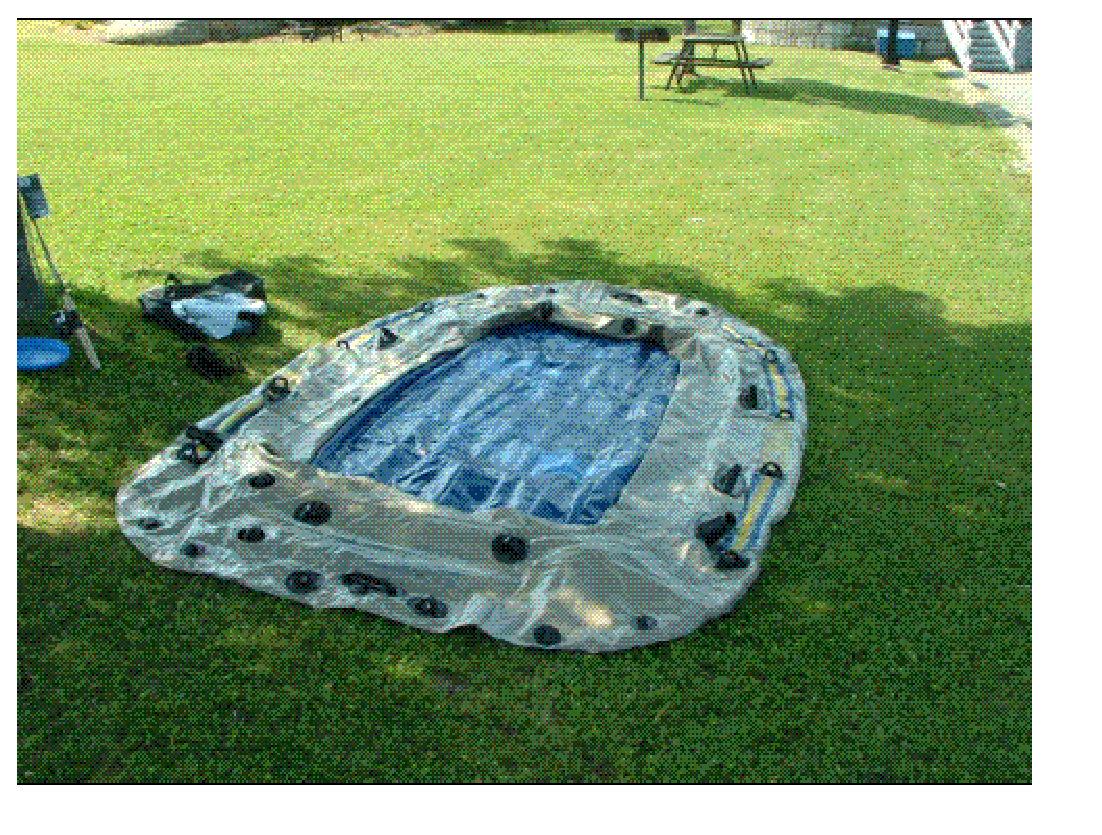
\epsfig{file=fig1.eps,width=3.5in}
Which one of the following is missing in it?
  
  
\noindent\hspace{3.0in} \begin{tabular}{|l|}
\hline
Your choice \\
\hline
 \\ 
 \\ 
\hline
\end{tabular}
  
  
 
 
\noindent{\textbf{\large{
A.}}}
A truck
 
 
\noindent{\textbf{\large{
B.}}}
A frisbee
 
 
\noindent{\textbf{\large{
C.}}}
Lawn
 
 
\noindent{\textbf{\large{
D.}}}
An air-boat
 
 
\noindent{\textbf{\large{
E.}}}
A table
 
 
\noindent{\textbf{\large{
F.}}}
  Not any of aboves.
 
 
 
\vspace{0.3in}
  
\vspace{0.2in}
  
         \begin{tabular}{|l|}
\hline
 Your marks  \\
\hline
 \\ 
 \\ 
\hline
\end{tabular}
\hspace{0.05in} \begin{tabular}{|l|}
\hline
 Full marks  \\
\hline
 \\ 
12.50 \\
\hline
\end{tabular}
{\textbf{\Large{Question
33.1.4 
}}}
  
  
What is the operation between $a= % 
7$ and $b= % 
8$:
$a$  % 
$\times$ $b=?$ Please also calculate it.

 
\vspace{0.3in}
  
\vspace{0.2in}
  
         \begin{tabular}{|l|}
\hline
 Your marks  \\
\hline
 \\ 
 \\ 
\hline
\end{tabular}
\hspace{0.05in} \begin{tabular}{|l|}
\hline
 Full marks  \\
\hline
 \\ 
12.50 \\
\hline
\end{tabular}
{\textbf{\Large{Question
33.1.5 
}}}
  
  
In a hotel, the possiblity of  % 
non-smoking customer is
$a =  % 
0.580$, and the possiblity of  % 
 under 30 years old customer is $ b =  % 
4.00 \times 10^{-2}$.
Please calculate the possiblity of  % 
smoking and  % 
equal or above 30 years old customer.
 

 

 
\vspace{0.3in}
  
\vspace{0.2in}
  
         \begin{tabular}{|l|}
\hline
 Your marks  \\
\hline
 \\ 
 \\ 
\hline
\end{tabular}
\hspace{0.05in} \begin{tabular}{|l|}
\hline
 Full marks  \\
\hline
 \\ 
12.50 \\
\hline
\end{tabular}
{\textbf{\Large{Question
33.1.6 
}}}
  
  
In a hotel, the possiblity of  % 
smoking customer is
$a =  % 
0.890$, and the possiblity of  % 
equal-or-above 30 years old customer is $ b =  % 
0.6400$.
Please fill the following form.
 
\noindent
\begin{tabular}{|l|l|}
\hline
Customer & Possibility \\
\hline
smoking  and   % 
equal-or-above 30 years old  & \\
\hline
smoking  and   % 
under 30 years old & \\
\hline
 non-smoking and   % 
equal-or-above 30 years old  & \\
\hline
 non-smoking and  % 
under 30 years old & \\
\hline
\end{tabular}
 
 
 

 

 
\vspace{0.3in}
   
   
\vspace{0.3in}
{\textbf{\LARGE{You have done all the above? A very good beginning, please go ahead.}}}
More constants the
Mass of electron
$m_e$$ =
9.109390 \times 10^{-31} $
kg
,
Universal gas constant
$R$$ =
8.315 $
J/(mol$\cdot $K)
,
$e$$ =
1.60217733 \times 10^{-19} $
C
, and
$m_p$$ =
1.6726231 \times 10^{-27} $
kg
%
may be very helpful.
\vspace{0.3in}
   
   
  
\vspace{0.2in}
  
\noindent\begin{tabular}{|l|}
\hline
 YOUR MARKS  \\
\hline
 \\ 
 \\ 
\hline
\end{tabular}
\hspace{0.05in} \begin{tabular}{|l|}
\hline
 Full Marks  \\
\hline
 \\ 
3.12 \\
\hline
\end{tabular}
{\textbf{\Large{QUESTION
33.2 
}}}
  
  
Considering case-insensitivity, please match the following same strings.
  
  
\begin{tabular}{|l|l|l|}
 \hline
 Column Left & Column Right  & Your choinces \\ 
 \hline
{\textbf{\large{
A.}}}
asdf(:)
  & 
c
 & 
 \\ 
 \hline
{\textbf{\large{
B.}}}
C
  & 
ER
 & 
 \\ 
 \hline
{\textbf{\large{
C.}}}
Er
  & 
b
 & 
 \\ 
 \hline
{\textbf{\large{
D.}}}
B
  & 
ASDF(:)
 & 
 \\ 
 \hline
{\textbf{\large{
E.}}}
A
  & 
a
 & 
 \\ 
 \hline
 \end{tabular}
  
  
 
  
\vspace{0.2in}
  
\noindent\begin{tabular}{|l|}
\hline
 YOUR MARKS  \\
\hline
 \\ 
 \\ 
\hline
\end{tabular}
\hspace{0.05in} \begin{tabular}{|l|}
\hline
 Full Marks  \\
\hline
 \\ 
1.56 \\
\hline
\end{tabular}
{\textbf{\Large{QUESTION
33.3 
}}}
  
  
Please choose the correct one from the following statements:
  
  
\noindent\hspace{3.0in} \begin{tabular}{|l|}
\hline
Your choice \\
\hline
 \\ 
 \\ 
\hline
\end{tabular}
  
  
 
 
\noindent{\textbf{\large{
A.}}}
Canada has  %
36 provinces and  %
35 territories.
 
 
\noindent{\textbf{\large{
B.}}}
Canada has  %
10 provinces and  %
3 territories.
 
 
\noindent{\textbf{\large{
C.}}}
Canada has  %
33 provinces and  %
38 territories.
 
 
\noindent{\textbf{\large{
D.}}}
Canada has  %
37 provinces and  %
37 territories.
 
 
\noindent{\textbf{\large{
E.}}}
Canada has  %
34 provinces and  %
39 territories.
 
 
\noindent{\textbf{\large{
F.}}}
 None of above.
 
 
  
\vspace{0.2in}
  
\noindent\begin{tabular}{|l|}
\hline
 YOUR MARKS  \\
\hline
 \\ 
 \\ 
\hline
\end{tabular}
\hspace{0.05in} \begin{tabular}{|l|}
\hline
 Full Marks  \\
\hline
 \\ 
1.56 \\
\hline
\end{tabular}
{\textbf{\Large{QUESTION
33.4 
}}}
  
  
 
An object is subjected to an external net force $\mathbf{f}=(
60.000 ,
4.0000,
-8000.0  )N$. Its mass is known as
$m= % 
54.0000  kg$. Please choose the correct accelaration
from the following choices.
 
  
  
\noindent\hspace{3.0in} \begin{tabular}{|l|}
\hline
Your choice \\
\hline
 \\ 
 \\ 
\hline
\end{tabular}
  
  
 
 
\noindent{\textbf{\large{
A.}}}
The accelaration is
$(
2.8796ms^{-2},
960.00km/h^2,
-689.97ms^{-2}
).
$
 
 
\noindent{\textbf{\large{
B.}}}
The accelaration is
$(
2.8796ms^{-2},
960.00km/h^2,
-148.15ms^{-2}
).
$
 
 
\noindent{\textbf{\large{
C.}}}
The accelaration is
$(
1.1111ms^{-2},
960.00km/h^2,
-689.97ms^{-2}
).
$
 
 
\noindent{\textbf{\large{
D.}}}
The accelaration is
$(
1.1111ms^{-2},
-4116.1km/h^2,
-148.15ms^{-2}
).
$
 
 
\noindent{\textbf{\large{
E.}}}
The accelaration is
$(
1.1111ms^{-2},
960.00km/h^2,
-148.15ms^{-2}
).
$
 
 
\noindent{\textbf{\large{
F.}}}
The accelaration is
$(
2.8796ms^{-2},
-4116.1km/h^2,
-148.15ms^{-2}
).
$
 
 
\noindent{\textbf{\large{
G.}}}
 None of these.
 
 
 
 

 
\vspace{0.3in}
  
\vspace{0.2in}
  
\noindent\begin{tabular}{|l|}
\hline
 YOUR MARKS  \\
\hline
 \\ 
 \\ 
\hline
\end{tabular}
\hspace{0.05in} \begin{tabular}{|l|}
\hline
 Full Marks  \\
\hline
 \\ 
3.12 \\
\hline
\end{tabular}
{\textbf{\Large{QUESTION
33.5 
}}}
  
  
 
 
An object is subjected to an external net force $\mathbf{f}=
(50.0 , 4.0 , -2000.0) N$.
Its mass is known as $m= % 
60.0000 kg$. Please choose the
correct accelaration from the following choices.
 
  
  
\noindent\hspace{3.0in} \begin{tabular}{|l|}
\hline
Your choice \\
\hline
 \\ 
 \\ 
\hline
\end{tabular}
  
  
 
 
\noindent{\textbf{\large{
A.}}}
The accelaration is $  %
(
0.833,
6.7 \times 10^{-2},
159.20)
ms^{-2} $.
 
 
\noindent{\textbf{\large{
B.}}}
The accelaration is $  %
(
0.833,
0.28,
-33.333)
ms^{-2} $.
 
 
\noindent{\textbf{\large{
C.}}}
The accelaration is $  %
(
0.833,
6.7 \times 10^{-2},
-33.333)
ms^{-2} $.
 
 
\noindent{\textbf{\large{
D.}}}
The accelaration is $  %
(
2.49,
0.28,
-33.333)
ms^{-2} $.
 
 
\noindent{\textbf{\large{
E.}}}
The accelaration is $  %
(
2.49,
6.7 \times 10^{-2},
-33.333)
ms^{-2} $.
 
 
\noindent{\textbf{\large{
F.}}}
The accelaration is $  %
(
2.49,
0.28,
159.20)
ms^{-2} $.
 
 
\noindent{\textbf{\large{
G.}}}
The accelaration is $  %
(
2.49,
6.7 \times 10^{-2},
159.20)
ms^{-2} $.
 
 
\noindent{\textbf{\large{
H.}}}
The accelaration is $  %
(
0.833,
0.28,
159.20)
ms^{-2} $.
 
 
 

 

 
\vspace{0.3in}
  
\vspace{0.2in}
  
\noindent\begin{tabular}{|l|}
\hline
 YOUR MARKS  \\
\hline
 \\ 
 \\ 
\hline
\end{tabular}
\hspace{0.05in} \begin{tabular}{|l|}
\hline
 Full Marks  \\
\hline
 \\ 
1.56 \\
\hline
\end{tabular}
{\textbf{\Large{QUESTION
33.6 
}}}
  
  
If any one of the following statements is correct, please fill the box ahead of it with $T$ .
If wrong, fill with $F$.
 
\noindent\begin{tabular}{|l|l|}\hline Your&\hspace{.2in} \\ answer&\hspace{.2in} \\ \hline \end{tabular}
1. $ % 
9$ is an  % 
even number.
 
\noindent\begin{tabular}{|l|l|}\hline Your&\hspace{.2in} \\ answer&\hspace{.2in} \\ \hline \end{tabular}
2.  % 
Toronto is in  % 
Ontario province.
 
\noindent\begin{tabular}{|l|l|}\hline Your&\hspace{.2in} \\ answer&\hspace{.2in} \\ \hline \end{tabular}
3.  % 
$\mathbf{F}=m\mathbf{a}$ is a mathmatical form of
the Newton's Second Law.
 

 
\vspace{0.3in}
   
   
\vspace{0.3in}
{\textbf{\LARGE{You have done all the above? Excellent! Not much left, please continue.}}}
\vspace{0.3in}
   
   
  
\vspace{0.2in}
  
\noindent\begin{tabular}{|l|}
\hline
 YOUR MARKS  \\
\hline
 \\ 
 \\ 
\hline
\end{tabular}
\hspace{0.05in} \begin{tabular}{|l|}
\hline
 Full Marks  \\
\hline
 \\ 
12.50 \\
\hline
\end{tabular}
{\textbf{\Large{QUESTION
33.7 
}}}
  
  
 
An object is subjected to an external net force $\mathbf{f}=
(70.0 , 9.0 , -7000.0) N$.
Its mass is known as $m= % 
58.0 kg$.
Please choose the correct accelaration from the following choices.
  
  
\noindent\hspace{3.0in} \begin{tabular}{|l|}
\hline
Your choice \\
\hline
 \\ 
 \\ 
\hline
\end{tabular}
  
  
 
 
\noindent{\textbf{\large{
A.}}}
  The accelaration is $  %
(
1.21,
0.16,
-120.69)
ms^{-2} $.
 
 
\noindent{\textbf{\large{
B.}}}
  The accelaration is $  %
(
4.23,
0.58,
-285.99)
ms^{-2} $.
 
 
\noindent{\textbf{\large{
C.}}}
  The accelaration is $  %
(
1.21,
0.16,
-285.99)
ms^{-2} $.
 
 
\noindent{\textbf{\large{
D.}}}
  The accelaration is $  %
(
4.23,
0.58,
-120.69)
ms^{-2} $.
 
 
 

 
 
\vspace{0.3in}
  
\vspace{0.2in}
  
\noindent\begin{tabular}{|l|}
\hline
 YOUR MARKS  \\
\hline
 \\ 
 \\ 
\hline
\end{tabular}
\hspace{0.05in} \begin{tabular}{|l|}
\hline
 Full Marks  \\
\hline
 \\ 
12.50 \\
\hline
\end{tabular}
{\textbf{\Large{QUESTION
33.8 
}}}
  
  
 
$ \left( \begin{array}{ccccccccc}
           5  & 
           6  & 
           6  & 
           4  \\ 
           4  & 
           5  & 
           6  & 
           6  \\ 
           7  & 
           5  & 
           4  & 
           5
\end{array}\right) \times
\left( \begin{array}{c}
           2  \\ 
           2  \\ 
           2  \\ 
           2
\end{array}\right) $ =?
 
 
$  % 
 \left( \begin{array}
 {
 c
 c
 }
 \Theta & 
 \Lambda \\ 
 \gamma & 
 \delta \\ 
 \Lambda & 
 \varepsilon \\ 
 \alpha & 
                    \Xi
 \end{array} \right)
 \left( \begin{array}
 {
 c
 }
 \beta \\ 
 \beta
 \end{array} \right)
$ =?
 

 

 
\vspace{0.3in}
  
\vspace{0.2in}
  
\noindent\begin{tabular}{|l|}
\hline
 YOUR MARKS  \\
\hline
 \\ 
 \\ 
\hline
\end{tabular}
\hspace{0.05in} \begin{tabular}{|l|}
\hline
 Full Marks  \\
\hline
 \\ 
1.56 \\
\hline
\end{tabular}
{\textbf{\Large{QUESTION
33.9 
}}}
  
  
 
 
% First root
% Second root

 
Please solve the following equation:
\begin{eqnarray*}
-11 \times x^2  % 
+  % 
737
                 \times x    % 
-12122 =0
\end{eqnarray*}
 

 

 
\vspace{0.3in}
   
   
 \vspace{0.2in}
Here are still some constants for use:
 
 
\noindent\begin{tabular}{|l|l|l|}
\hline
Constant & Symbol & Value \\
\hline
 
Mass of proton &
$m_p$ &
 $ 1.6726231 \times 10^{-27} $
kg \\
\hline
 
Boltzmann's constant &
$k$ &
 $ 1.381 \times 10^{-23} $
J/K \\
\hline
 
\end{tabular}
 
Thank you very much for answering these questions!
 
{\textbf{\large{Please be advised}}} that in this paper there are questions from
33.1 through
33.9.
And any one of them may contain more than one sub-question, thus the total number
of sub-questions here is around 14, of which
13 should be answered.
 
   
   
   
   
\vspace{1.0in} 
{\textbf{\large{ *** END OF PAPER, THANKS *** }}} 
   
   
\hspace{1.0in} By: 
         239 (          26 ,           34 )
   
   
   
   
\newpage 
\setcounter{page}{ 
    34001 } 
   
   
   
   
\noindent\begin{tabular}{|l|}
\hline
YOUR NAME (FIRST, ... LAST)  \\
\hline
 \\ 
 \\ 
\hline
\end{tabular}
\hspace{0.05in} \begin{tabular}{|l|}
\hline
 YOUR   ID   INFORMATION  \\
\hline
 \\ 
 \\ 
\hline
\end{tabular}
   
   
\vspace{0.2in}\noindent\begin{tabular}{|l|}
\hline
YOUR TOTAL MARKS  \\
\hline
 \\ 
 \\ 
\hline
\end{tabular}
\hspace{0.05in} \begin{tabular}{|l|}
\hline
TOTAL FULL MARKS  \\
\hline
 \\ 
100.00 \\
\hline
\end{tabular}
   
   
 \vspace{0.2in}
 
 
{\Huge  THIS IS AN EXAMPLE OF}
 
{\Huge  PERSONALIZED TESTS. }
 
If needed, please use the following constants.
 
 
 
\noindent\begin{tabular}{|l|l|l|}
\hline
Constant & Symbol & Value \\
\hline
Acceleration due to earth's gravity &
$g$ &
 $ 9.80 $
m/s$^2$ \\
\hline
Avogadro's number &
$N_A$ &
 $ 6.0221367 \times 10^{23} $
mol$^{-1}$ \\
\hline
Boltzmann's constant &
$k$ &
 $ 1.380658 \times 10^{-23} $
J/K \\
\hline
Coulomb's constant &
$k$ &
 $ 8.99 \times 10^{9} $
N$\cdot $m$^2$/C$^2$ \\
\hline
Electron charge magnitiude &
$e$ &
 $ 1.60217733 \times 10^{-19} $
C \\
\hline
Permeability of free space &
$\mu _0$ &
 $ 1.25663706 \times 10^{-6} $
T$\cdot $m/A \\
\hline
Permittivity of free space &
$\epsilon _0$ &
 $ 8.854187817 \times 10^{-12} $
C$^2$/(N$\cdot $m$^2$) \\
\hline
Pi &
$\pi$ &
 $ 3.14159265 $
$ $ \\
\hline
Planck's constant &
$h$ &
 $ 6.6260755 \times 10^{-34} $
J$\cdot $s \\
\hline
Mass of electron &
$m_e$ &
 $ 9.1093897 \times 10^{-31} $
kg \\
\hline
\end{tabular}
 
 
\noindent\begin{tabular}{|l|l|l|}
\hline
Constant & Symbol & Value \\
\hline
Mass of neutron &
$m_n$ &
 $ 1.6749286 \times 10^{-27} $
kg \\
\hline
Mass of proton &
$m_p$ &
 $ 1.6726231 \times 10^{-27} $
kg \\
\hline
Speed of light in vacuum &
$c$ &
 $ 299792458. $
m/s \\
\hline
Universal gravitational constant &
$G$ &
 $ 6.67259 \times 10^{-11} $
N$\cdot $m$^2$/kg$^2$ \\
\hline
Universal gas constant &
$R$ &
 $ 8.314510 $
J/(mol$\cdot $K) \\
\hline
\end{tabular}
 
 
{\textbf{\large{Please be advised}}} that in this paper there are questions from
34.1 through
34.9.
And any one of them may contain more than one sub-question, thus the total number
of sub-questions here is around 14, of which
13 should be answered.
 
\vspace{0.3in}
 
 
   
   
  
\vspace{0.2in}
  
\noindent\begin{tabular}{|l|}
\hline
 YOUR MARKS  \\
\hline
 \\ 
 \\ 
\hline
\end{tabular}
\hspace{0.05in} \begin{tabular}{|l|}
\hline
 Full Marks  \\
\hline
 \\ 
62.50 \\
\hline
\end{tabular}
{\textbf{\Large{QUESTION
34.1 
}}}
  
  
 
{\textbf{\Large{Please answer ONLY
5 of the following
6 questions (Questions
34.1.1 through
34.1.6). }}}
 
Here are still some constants for use in the following questions:
 
 
\noindent\begin{tabular}{|l|l|l|}
\hline
Constant & Symbol & Value \\
\hline
 
Boltzmann's constant &
$k$ &
 $ 1.381 \times 10^{-23} $
J/K \\
\hline
 
Avogadro's number &
$N_A$ &
 $ 6.022 \times 10^{23} $
mol$^{-1}$ \\
\hline
 
Mass of electron &
$m_e$ &
 $ 9.1093897 \times 10^{-31} $
kg \\
\hline
 
\end{tabular}
 
  
\vspace{0.2in}
  
         \begin{tabular}{|l|}
\hline
 Your marks  \\
\hline
 \\ 
 \\ 
\hline
\end{tabular}
\hspace{0.05in} \begin{tabular}{|l|}
\hline
 Full marks  \\
\hline
 \\ 
12.50 \\
\hline
\end{tabular}
{\textbf{\Large{Question
34.1.1 
}}}
  
  
 
An object is subjected to an external net force $\mathbf{f}=(
80.0,  % 
4.0,
-2000.0  )N$. Its mass is known as
$m= % 
52.0 kg$. Please calculate its accelaration.
 
 

 

 
\vspace{0.3in}
  
\vspace{0.2in}
  
         \begin{tabular}{|l|}
\hline
 Your marks  \\
\hline
 \\ 
 \\ 
\hline
\end{tabular}
\hspace{0.05in} \begin{tabular}{|l|}
\hline
 Full marks  \\
\hline
 \\ 
12.50 \\
\hline
\end{tabular}
{\textbf{\Large{Question
34.1.2 
}}}
  
  
In a hotel, the possiblity of  % 
smoking customer is
$a =  % 
0.290$, and the possiblity of  % 
equal or above 30 years old customer is $ b =  % 
0.3200$.
Please calculate the possiblity of  % 
 non-smoking and  % 
under 30 years old customer.
 

 

 
\vspace{0.3in}
  
\vspace{0.2in}
  
         \begin{tabular}{|l|}
\hline
 Your marks  \\
\hline
 \\ 
 \\ 
\hline
\end{tabular}
\hspace{0.05in} \begin{tabular}{|l|}
\hline
 Full marks  \\
\hline
 \\ 
12.50 \\
\hline
\end{tabular}
{\textbf{\Large{Question
34.1.3 
}}}
  
  
In a hotel, the possiblity of  % 
smoking customer is
$a =  % 
0.480$, and the possiblity of  % 
equal-or-above 30 years old customer is $ b =  % 
0.4400$.
Please fill the following form.
 
\noindent
\begin{tabular}{|l|l|}
\hline
Customer & Possibility \\
\hline
smoking  and   % 
equal-or-above 30 years old  & \\
\hline
smoking  and   % 
under 30 years old & \\
\hline
 non-smoking and   % 
equal-or-above 30 years old  & \\
\hline
 non-smoking and  % 
under 30 years old & \\
\hline
\end{tabular}
 
 
 

 

 
\vspace{0.3in}
  
\vspace{0.2in}
  
         \begin{tabular}{|l|}
\hline
 Your marks  \\
\hline
 \\ 
 \\ 
\hline
\end{tabular}
\hspace{0.05in} \begin{tabular}{|l|}
\hline
 Full marks  \\
\hline
 \\ 
12.50 \\
\hline
\end{tabular}
{\textbf{\Large{Question
34.1.4 
}}}
  
  
 
An object is subjected to an external net force $\mathbf{f}=(
20.0 ,
4.0,
-8000.0  )N$. Its mass is known as
$m= % 
54.0  kg$. Please choose the correct accelaration
from the following choices.
 
  
  
\noindent\hspace{3.0in} \begin{tabular}{|l|}
\hline
Your choice \\
\hline
 \\ 
 \\ 
\hline
\end{tabular}
  
  
 
 
\noindent{\textbf{\large{
A.}}}
The accelaration is
$(
0.37037ms^{-2},
0.33040ms^{-2},
6.8548 \times 10^{6}km/h^2
).
$
 
 
\noindent{\textbf{\large{
B.}}}
The accelaration is
$(
0.37037ms^{-2},
7.4074 \times 10^{-2}ms^{-2},
6.8548 \times 10^{6}km/h^2
).
$
 
 
\noindent{\textbf{\large{
C.}}}
The accelaration is
$(
0.37037ms^{-2},
0.33040ms^{-2},
-1.9200 \times 10^{6}km/h^2
).
$
 
 
\noindent{\textbf{\large{
D.}}}
The accelaration is
$(
0.95015ms^{-2},
0.33040ms^{-2},
6.8548 \times 10^{6}km/h^2
).
$
 
 
\noindent{\textbf{\large{
E.}}}
none of these.
 
 
 
 

 
\vspace{0.3in}
  
\vspace{0.2in}
  
         \begin{tabular}{|l|}
\hline
 Your marks  \\
\hline
 \\ 
 \\ 
\hline
\end{tabular}
\hspace{0.05in} \begin{tabular}{|l|}
\hline
 Full marks  \\
\hline
 \\ 
12.50 \\
\hline
\end{tabular}
{\textbf{\Large{Question
34.1.5 
}}}
  
  
 
An object is subjected to an external net force $\mathbf{f}=(
30.0 ,
9.0,
-9000.0  )N$. Its mass is known as
$m= % 
52.0  kg$. Please choose the correct accelaration
from the following choices.
 
  
  
\noindent\hspace{3.0in} \begin{tabular}{|l|}
\hline
Your choice \\
\hline
 \\ 
 \\ 
\hline
\end{tabular}
  
  
 
 
\noindent{\textbf{\large{
A.}}}
The accelaration (vector) is
$(
7476.9,
2243.1 ,
7.6349 \times 10^{6}
)km/h^2.
$
 
 
\noindent{\textbf{\large{
B.}}}
The accelaration (vector) is
$(
22007.,
2243.1 ,
6.8282 \times 10^{6}
)km/h^2.
$
 
 
\noindent{\textbf{\large{
C.}}}
The accelaration (vector) is
$(
27105.,
2243.1 ,
-2.2431 \times 10^{6}
)km/h^2.
$
 
 
\noindent{\textbf{\large{
D.}}}
The accelaration (vector) is
$(
7476.9,
2243.1 ,
-2.2431 \times 10^{6}
)km/h^2.
$
 
 
\noindent{\textbf{\large{
E.}}}
The accelaration (vector) is
$(
23622.,
2243.1 ,
6.8282 \times 10^{6}
)km/h^2.
$
 
 
\noindent{\textbf{\large{
F.}}}
The accelaration (vector) is
$(
27105.,
2243.1 ,
7.6349 \times 10^{6}
)km/h^2.
$
 
 
\noindent{\textbf{\large{
G.}}}
The accelaration (vector) is
$(
22007.,
2243.1 ,
7.6349 \times 10^{6}
)km/h^2.
$
 
 
\noindent{\textbf{\large{
H.}}}
The accelaration (vector) is
$(
27105.,
2243.1 ,
8.9406 \times 10^{6}
)km/h^2.
$
 
 
\noindent{\textbf{\large{
I.}}}
The accelaration (vector) is
$(
23622.,
2243.1 ,
-2.2431 \times 10^{6}
)km/h^2.
$
 
 
\noindent{\textbf{\large{
J.}}}
The accelaration (vector) is
$(
22007.,
2243.1 ,
-2.2431 \times 10^{6}
)km/h^2.
$
 
 
\noindent{\textbf{\large{
K.}}}
The accelaration (vector) is
$(
7476.9,
2243.1 ,
6.8282 \times 10^{6}
)km/h^2.
$
 
 
\noindent{\textbf{\large{
L.}}}
The accelaration (vector) is
$(
23622.,
2243.1 ,
8.9406 \times 10^{6}
)km/h^2.
$
 
 
 
 

 
 
\vspace{0.3in}
  
\vspace{0.2in}
  
         \begin{tabular}{|l|}
\hline
 Your marks  \\
\hline
 \\ 
 \\ 
\hline
\end{tabular}
\hspace{0.05in} \begin{tabular}{|l|}
\hline
 Full marks  \\
\hline
 \\ 
12.50 \\
\hline
\end{tabular}
{\textbf{\Large{Question
34.1.6 
}}}
  
  
What is the operation between $a= % 
1$ and $b= % 
4$:
$a$  % 
$\times$ $b=?$ Please also calculate it.

 
\vspace{0.3in}
   
   
\vspace{0.3in}
{\textbf{\LARGE{You have done all the above? A very good beginning, please go ahead.}}}
More constants the
Mass of electron
$m_e$$ =
9.109390 \times 10^{-31} $
kg
,
Universal gas constant
$R$$ =
8.315 $
J/(mol$\cdot $K)
,
$e$$ =
1.60217733 \times 10^{-19} $
C
, and
$m_p$$ =
1.6726231 \times 10^{-27} $
kg
%
may be very helpful.
\vspace{0.3in}
   
   
  
\vspace{0.2in}
  
\noindent\begin{tabular}{|l|}
\hline
 YOUR MARKS  \\
\hline
 \\ 
 \\ 
\hline
\end{tabular}
\hspace{0.05in} \begin{tabular}{|l|}
\hline
 Full Marks  \\
\hline
 \\ 
1.56 \\
\hline
\end{tabular}
{\textbf{\Large{QUESTION
34.2 
}}}
  
  
If any one of the following statements is correct, please fill the box ahead of it with $T$ .
If wrong, fill with $F$.
 
\noindent\begin{tabular}{|l|l|}\hline Your&\hspace{.2in} \\ answer&\hspace{.2in} \\ \hline \end{tabular}
1. $ % 
74$ is an  % 
even number.
 
\noindent\begin{tabular}{|l|l|}\hline Your&\hspace{.2in} \\ answer&\hspace{.2in} \\ \hline \end{tabular}
2.  % 
Toronto is in  % 
Ontario province.
 
\noindent\begin{tabular}{|l|l|}\hline Your&\hspace{.2in} \\ answer&\hspace{.2in} \\ \hline \end{tabular}
3.  % 
$\left| \mathbf{F}\right| =Gm_1m_2r^{-2}$ is a mathmatical form of
Newton's Law of Universal Gravitation.
 

 
\vspace{0.3in}
  
\vspace{0.2in}
  
\noindent\begin{tabular}{|l|}
\hline
 YOUR MARKS  \\
\hline
 \\ 
 \\ 
\hline
\end{tabular}
\hspace{0.05in} \begin{tabular}{|l|}
\hline
 Full Marks  \\
\hline
 \\ 
1.56 \\
\hline
\end{tabular}
{\textbf{\Large{QUESTION
34.3 
}}}
  
  
Please choose the correct one from the following statements:
  
  
\noindent\hspace{3.0in} \begin{tabular}{|l|}
\hline
Your choice \\
\hline
 \\ 
 \\ 
\hline
\end{tabular}
  
  
 
 
\noindent{\textbf{\large{
A.}}}
Canada has  %
34 provinces and  %
39 territories.
 
 
\noindent{\textbf{\large{
B.}}}
Canada has  %
37 provinces and  %
37 territories.
 
 
\noindent{\textbf{\large{
C.}}}
Canada has  %
36 provinces and  %
35 territories.
 
 
\noindent{\textbf{\large{
D.}}}
Canada has  %
33 provinces and  %
38 territories.
 
 
\noindent{\textbf{\large{
E.}}}
Canada has  %
10 provinces and  %
3 territories.
 
 
\noindent{\textbf{\large{
F.}}}
 None of above.
 
 
  
\vspace{0.2in}
  
\noindent\begin{tabular}{|l|}
\hline
 YOUR MARKS  \\
\hline
 \\ 
 \\ 
\hline
\end{tabular}
\hspace{0.05in} \begin{tabular}{|l|}
\hline
 Full Marks  \\
\hline
 \\ 
3.12 \\
\hline
\end{tabular}
{\textbf{\Large{QUESTION
34.4 
}}}
  
  
 
 
An object is subjected to an external net force $\mathbf{f}=
(90.0 , 8.0 , -4000.0) N$.
Its mass is known as $m= % 
58.0000 kg$. Please choose the
correct accelaration from the following choices.
 
  
  
\noindent\hspace{3.0in} \begin{tabular}{|l|}
\hline
Your choice \\
\hline
 \\ 
 \\ 
\hline
\end{tabular}
  
  
 
 
\noindent{\textbf{\large{
A.}}}
The accelaration is $  %
(
4.69,
0.14,
247.31)
ms^{-2} $.
 
 
\noindent{\textbf{\large{
B.}}}
The accelaration is $  %
(
1.55,
0.43,
-68.966)
ms^{-2} $.
 
 
\noindent{\textbf{\large{
C.}}}
The accelaration is $  %
(
4.69,
0.43,
247.31)
ms^{-2} $.
 
 
\noindent{\textbf{\large{
D.}}}
The accelaration is $  %
(
4.69,
0.14,
-68.966)
ms^{-2} $.
 
 
\noindent{\textbf{\large{
E.}}}
The accelaration is $  %
(
1.55,
0.43,
247.31)
ms^{-2} $.
 
 
\noindent{\textbf{\large{
F.}}}
The accelaration is $  %
(
1.55,
0.14,
247.31)
ms^{-2} $.
 
 
\noindent{\textbf{\large{
G.}}}
The accelaration is $  %
(
1.55,
0.14,
-68.966)
ms^{-2} $.
 
 
\noindent{\textbf{\large{
H.}}}
The accelaration is $  %
(
4.69,
0.43,
-68.966)
ms^{-2} $.
 
 
 

 

 
\vspace{0.3in}
  
\vspace{0.2in}
  
\noindent\begin{tabular}{|l|}
\hline
 YOUR MARKS  \\
\hline
 \\ 
 \\ 
\hline
\end{tabular}
\hspace{0.05in} \begin{tabular}{|l|}
\hline
 Full Marks  \\
\hline
 \\ 
3.12 \\
\hline
\end{tabular}
{\textbf{\Large{QUESTION
34.5 
}}}
  
  
Considering case-insensitivity, please match the following same strings.
  
  
\begin{tabular}{|l|l|l|}
 \hline
 Column Left & Column Right  & Your choinces \\ 
 \hline
{\textbf{\large{
A.}}}
asdf(:)
  & 
a
 & 
 \\ 
 \hline
{\textbf{\large{
B.}}}
Er
  & 
b
 & 
 \\ 
 \hline
{\textbf{\large{
C.}}}
A
  & 
eR
 & 
 \\ 
 \hline
{\textbf{\large{
D.}}}
B
  & 
ASDF(:)
 & 
 \\ 
 \hline
{\textbf{\large{
E.}}}
 A= %
4/ %
2

  & 
 a= %
2
 & 
 \\ 
 \hline
 \end{tabular}
  
  
 
  
\vspace{0.2in}
  
\noindent\begin{tabular}{|l|}
\hline
 YOUR MARKS  \\
\hline
 \\ 
 \\ 
\hline
\end{tabular}
\hspace{0.05in} \begin{tabular}{|l|}
\hline
 Full Marks  \\
\hline
 \\ 
1.56 \\
\hline
\end{tabular}
{\textbf{\Large{QUESTION
34.6 
}}}
  
  
 
An object is subjected to an external net force $\mathbf{f}=(
70.000 ,
3.0000,
-9000.0  )N$. Its mass is known as
$m= % 
50.0000  kg$. Please choose the correct accelaration
from the following choices.
 
  
  
\noindent\hspace{3.0in} \begin{tabular}{|l|}
\hline
Your choice \\
\hline
 \\ 
 \\ 
\hline
\end{tabular}
  
  
 
 
\noindent{\textbf{\large{
A.}}}
The accelaration is
$(
1.4000ms^{-2},
-3171.4km/h^2,
-180.00ms^{-2}
).
$
 
 
\noindent{\textbf{\large{
B.}}}
The accelaration is
$(
1.4000ms^{-2},
777.60km/h^2,
-180.00ms^{-2}
).
$
 
 
\noindent{\textbf{\large{
C.}}}
The accelaration is
$(
5.5031ms^{-2},
-3171.4km/h^2,
798.44ms^{-2}
).
$
 
 
\noindent{\textbf{\large{
D.}}}
The accelaration is
$(
1.4000ms^{-2},
-3171.4km/h^2,
798.44ms^{-2}
).
$
 
 
\noindent{\textbf{\large{
E.}}}
The accelaration is
$(
5.5031ms^{-2},
777.60km/h^2,
798.44ms^{-2}
).
$
 
 
\noindent{\textbf{\large{
F.}}}
The accelaration is
$(
1.4000ms^{-2},
777.60km/h^2,
798.44ms^{-2}
).
$
 
 
\noindent{\textbf{\large{
G.}}}
 None of these.
 
 
 
 

 
\vspace{0.3in}
   
   
\vspace{0.3in}
{\textbf{\LARGE{You have done all the above? Excellent! Not much left, please continue.}}}
\vspace{0.3in}
   
   
  
\vspace{0.2in}
  
\noindent\begin{tabular}{|l|}
\hline
 YOUR MARKS  \\
\hline
 \\ 
 \\ 
\hline
\end{tabular}
\hspace{0.05in} \begin{tabular}{|l|}
\hline
 Full Marks  \\
\hline
 \\ 
12.50 \\
\hline
\end{tabular}
{\textbf{\Large{QUESTION
34.7 
}}}
  
  
 
$ \left( \begin{array}{ccccccccc}
           5  & 
           4  & 
           4  & 
           6  \\ 
           6  & 
           4  & 
           6  & 
           4  \\ 
           5  & 
           4  & 
           5  & 
           5
\end{array}\right) \times
\left( \begin{array}{c}
           2  \\ 
           2  \\ 
           2  \\ 
           2
\end{array}\right) $ =?
 
 
$  % 
 \left( \begin{array}
 {
 c
 c
 }
 \Delta & 
 \rho \\ 
 \eta & 
 \rho \\ 
                    \Xi & 
 \sigma \\ 
 \varepsilon & 
 \epsilon
 \end{array} \right)
 \left( \begin{array}
 {
 c
 }
 \beta \\ 
 \beta
 \end{array} \right)
$ =?
 

 

 
\vspace{0.3in}
  
\vspace{0.2in}
  
\noindent\begin{tabular}{|l|}
\hline
 YOUR MARKS  \\
\hline
 \\ 
 \\ 
\hline
\end{tabular}
\hspace{0.05in} \begin{tabular}{|l|}
\hline
 Full Marks  \\
\hline
 \\ 
12.50 \\
\hline
\end{tabular}
{\textbf{\Large{QUESTION
34.8 
}}}
  
  
 
An object is subjected to an external net force $\mathbf{f}=
(80.0 , 3.0 , -9000.0) N$.
Its mass is known as $m= % 
52.0 kg$.
Please choose the correct accelaration from the following choices.
  
  
\noindent\hspace{3.0in} \begin{tabular}{|l|}
\hline
Your choice \\
\hline
 \\ 
 \\ 
\hline
\end{tabular}
  
  
 
 
\noindent{\textbf{\large{
A.}}}
  The accelaration is $  %
(
6.33,
5.8 \times 10^{-2},
-173.08)
ms^{-2} $.
 
 
\noindent{\textbf{\large{
B.}}}
  The accelaration is $  %
(
1.54,
5.8 \times 10^{-2},
786.99)
ms^{-2} $.
 
 
\noindent{\textbf{\large{
C.}}}
  The accelaration is $  %
(
6.33,
0.17,
-173.08)
ms^{-2} $.
 
 
\noindent{\textbf{\large{
D.}}}
  The accelaration is $  %
(
1.54,
5.8 \times 10^{-2},
-173.08)
ms^{-2} $.
 
 
 

 
 
\vspace{0.3in}
  
\vspace{0.2in}
  
\noindent\begin{tabular}{|l|}
\hline
 YOUR MARKS  \\
\hline
 \\ 
 \\ 
\hline
\end{tabular}
\hspace{0.05in} \begin{tabular}{|l|}
\hline
 Full Marks  \\
\hline
 \\ 
1.56 \\
\hline
\end{tabular}
{\textbf{\Large{QUESTION
34.9 
}}}
  
  
 
 
% First root
% Second root

 
Please solve the following equation:
\begin{eqnarray*}
-5 \times x^2  % 
+  % 
85
                 \times x    % 
+  % 
300 =0
\end{eqnarray*}
 

 

 
\vspace{0.3in}
   
   
 \vspace{0.2in}
Here are still some constants for use:
 
 
\noindent\begin{tabular}{|l|l|l|}
\hline
Constant & Symbol & Value \\
\hline
 
Mass of proton &
$m_p$ &
 $ 1.6726231 \times 10^{-27} $
kg \\
\hline
 
Boltzmann's constant &
$k$ &
 $ 1.381 \times 10^{-23} $
J/K \\
\hline
 
\end{tabular}
 
Thank you very much for answering these questions!
 
{\textbf{\large{Please be advised}}} that in this paper there are questions from
34.1 through
34.9.
And any one of them may contain more than one sub-question, thus the total number
of sub-questions here is around 14, of which
13 should be answered.
 
   
   
   
   
\vspace{1.0in} 
{\textbf{\large{ *** END OF PAPER, THANKS *** }}} 
   
   
\hspace{1.0in} By: 
         239 (          26 ,           34 )
   
   
 
 
\end{document}
